% !TeX program = xelatex
% !TeX encoding = UTF-8
\documentclass[final,5p,times,twocolumn]{elsarticle}

\usepackage{iftex}
\ifXeTeX\else
  \PackageError{JMS_Review_CN}{This manuscript requires XeLaTeX}
    {Select XeLaTeX as the compiler and compile again.}
\fi
\IfFileExists{ctex-fontset-fandol.def}
  {\usepackage[UTF8,scheme=plain,fontset=fandol]{ctex}}
  {\usepackage[UTF8,scheme=plain,fontset=windows]{ctex}}
\usepackage{amsmath,amssymb,mathtools}
\usepackage{booktabs,array,multirow}
\newcolumntype{C}[1]{>{\centering\arraybackslash}m{#1}}
\usepackage{graphicx}
\usepackage{enumitem}
\usepackage{placeins}
\usepackage{dblfloatfix}
\usepackage{flafter}
\usepackage{microtype}
  \usepackage{xurl}
  \usepackage{xcolor}
\definecolor{JMSCiteBlue}{HTML}{0072B2}
\usepackage[colorlinks=true,citecolor=JMSCiteBlue,linkcolor=JMSCiteBlue,urlcolor=JMSCiteBlue]{hyperref}
\graphicspath{{figures/terminology_cn/}{figures/}}
\setlength{\emergencystretch}{3em}
\setcounter{topnumber}{2}
\setcounter{dbltopnumber}{1}
\setcounter{dblbotnumber}{1}
\renewcommand{\topfraction}{0.90}
\renewcommand{\dbltopfraction}{0.72}
\renewcommand{\textfraction}{0.10}
\renewcommand{\floatpagefraction}{0.90}
\renewcommand{\dblfloatpagefraction}{0.95}

\journal{Journal of Manufacturing Systems}
\biboptions{sort&compress}

\newcommand{\method}{RDMCT-HBS}
\newcommand{\cmax}{C_{\max}}
\newcommand{\pdi}{\mathrm{PDI}}
\newcounter{algorithm}
\newcommand{\algorithmtitle}[1]{\refstepcounter{algorithm}\noindent\textbf{算法~\thealgorithm：#1}\par\smallskip}

\begin{document}
\begin{frontmatter}

\title{双源混流旋转腔组合设备在满片加工下的两阶段调度}

\author[ustb]{邵立珍（Lizhen Shao）\corref{cor1}}
\ead{lshao@ustb.edu.cn}
\author[ustb]{魏林聪（Lincong Wei）}
\author[ustb]{王蔚（Wei Wang）}

\cortext[cor1]{通讯作者。}
\address[ustb]{北京科技大学控制科学与工程系，北京市海淀区学院路30号，
北京100083，中国}

\begin{abstract}
先进制程提高了薄膜沉积工艺对产能、空间利用率与稳定运行的要求，促使组合设备向多空间旋转腔发展。其中含碳薄
膜工艺难清理残留使得空工位在加工和清洗期间面临污染风险，需要辅助晶圆补齐工位。辅助晶圆与产品晶圆存储在不
同区域，在共享机械手与多工位旋转腔中形成混流。本文建立两阶段混合整数线性规划模型，第一阶段在驻留上限等物
理约束下缩短产品批次完工时间，第二阶段保留其上界及主要结构，减少等待并抑制相邻生产周期的节拍变化。采用结
构化初始化、限时MILP搜索和时序精修，并评估学习割选择的作用。历史固定布局下，16片批次在清洁阈值为3、4和6
时满片加工的最优工艺模式分别为纯$4\times1$、混合和纯$2\times2$。四组配置各三个种子的冷启动均未在300~s
内取得可行解，采用预计算初始解的主求解均获得有效排程；八组等预算精修保持产品完工时间，并使总等待降低
22.29\%--50.25\%。另在四组具有有效节拍评价中心的纯$2\times2$配置中，总等待下降41.53\%--58.50\%，但未观察到超过数值容差的节拍改善。研究为满片工艺下的旋转腔组合设备调度的模式比较及有限预算内可行排程的获取提供了统一的
建模与评价方法。

\end{abstract}

\begin{keyword}
半导体制造系统 \sep 满片工艺 \sep 假片调度 \sep 两阶段优化 \sep 混合整数线性规划 \sep 学习增强精确优化
\end{keyword}

\end{frontmatter}
\section{引言}

等离子体增强化学气相沉积（plasma-enhanced chemical vapor deposition，PECVD）用于半导体薄膜制备。组合设备（cluster tool，CT）将工艺模块、机械手和装载锁连接为连续的晶圆处理路径。工艺处理与搬运时间、装载锁切换、腔室清洁和驻留约束共同决定设备的可行运行时序及产出\citep{pan2018survey}。三维器件结构与多层薄膜集成对沉积均匀性和工艺处理能力提出了更高要求\citep{appliedprecisioncvd}，多空间工艺模块与多指机械手则为提高单个设备内的并行处理能力提供了结构基础\citep{gu2024applied,gu2024multifinger}。

本文研究具有四工位旋转腔的PECVD组合设备，其运行决策起点是所研究配方的满片要求：生产时四个工位均须由晶圆占用，产品不足时用假片补位。本文将用于生产补位或清洁占位、归还后可复用的假片统一称为辅助晶圆（dummy wafer）。假片不计入产品产出，但其取放、旋转、搬运及重复借用会占用设备资源。产品晶圆从大气侧装载端口进入，经对准和装载锁送至腔室；双源配置中的辅助晶圆由真空存储区供给。两类晶圆的来源和路线差异是模式比较需要纳入的设备条件。

\begin{figure}[t]
\centering
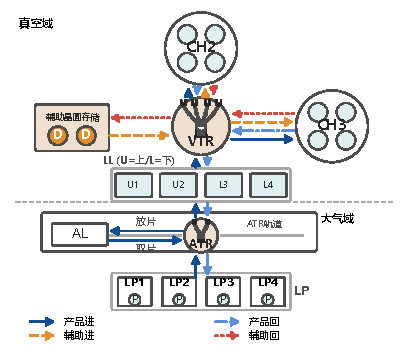
\includegraphics[width=\linewidth]{fig_system_cn_nature}
\caption{双源混流旋转腔组合设备拓扑与晶圆运行路线。}
\label{fig:system-zh-new}
\end{figure}

\begin{figure}[!htbp]
\centering
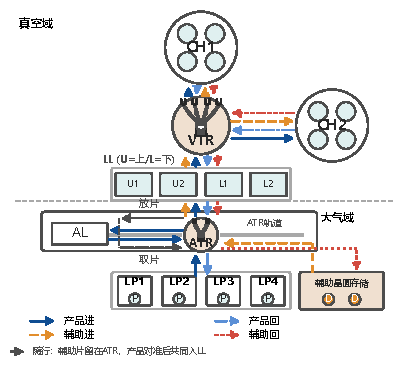
\includegraphics[width=\linewidth]{fig_single_source_cn}
\caption{单源旋转腔设备的拓扑与晶圆路线。辅助存储位于LP4旁。产品经AL对准后进入上装载锁；辅助晶圆单独供给时由ATR直接送入上装载锁，与产品共同取片时随行至AL并保持在ATR上，待产品完成对准后共同送入上装载锁。两类晶圆经VTR进入腔室，经下装载锁和ATR返回各自存储位。}
\label{fig:single-source-cn}
\end{figure}


满片占用使产品供给与辅助晶圆复用相互制约。产品不足以填满工位时，辅助晶圆承担补位；清洁占用辅助晶圆与腔室，并改变后续可用时刻。因此，产品到达腔室并不意味着能够立即开始工艺处理，还需满足辅助晶圆可用性、机械手服务次序和清洁边界等条件。图~\ref{fig:system-zh-new}中的两类晶圆路线需要在同一排程中协调。

设备的生产过程采用$4\times1$并行生产与$2\times2$链式生产两种预设工艺模式。前者使四片晶圆同步完成一次工艺处理，后者通过成对装卸与旋转使每片产品连续参加两次工艺处理。两种模式由配方及腔室操作方式规定；满片要求引入的假片使其批次补位、链首链尾占位及清洁衔接产生不同的资源代价。因此，相同的产品累计名义工艺时长并不意味着相同的批次完工时间，模式优选需要结合批量、清洁阈值、假片供给和搬运条件判定。每次求解中产品模式由输入给定；本文通过分别构造纯模式和混合配置、比较可验证排程及其上下界来支持模式选择，而非在一次求解中自由改变产品配方。

已有CT研究建立了工艺处理、搬运与吞吐率之间的解析关系\citep{perkinson1994throughput}，并通过线性规划、启发式和时间Petri网求解带驻留约束的排程\citep{rostami2002optimal,wu2010closedform,qiao2012sojourn}。研究范围进一步扩展到重入工艺、多类晶圆和可选工艺模块\citep{qiao2014revisiting,wang2020multiple,wang2025virtualcell}。四指机械手与四空间模块的洁净/脏手分工及稳态周期分析，以及两类晶圆投放与搬运的联合优化，为复杂设备结构提供了建模基础\citep{gu2024multifinger,yang2025miptwowafers}。有限批次还包含链首初始化、链尾退出和末批补位，辅助晶圆的返回时刻因此直接影响后续生产。

周期清洁调度采用任务序列枚举、部分装载与时刻控制、虚拟晶圆占位和腔室状态触发等方式协调清洁与生产\citep{kim2013cleaning,yu2020delay,qiao2022binary,li2022conditioncleaning}。共享缓冲同步和动态动作筛选用于避免故障停机与非周期运行中的死锁\citep{zhu2025failuredeadlock,kim2025noncyclicdeadlock}，等待约束还关系到设备产出和上游控制\citep{lee2018waiting}。对本文设备而言，清洁同时改变生产链分段、辅助晶圆占用和真空机械手次序，单独安排产品工艺处理或清洁时刻难以完整表示这些依赖关系。

制造系统的时序质量还要求区分批次效率与工序衔接。JMS关于等待约束的研究将允许等待与有效产出联系起来\citep{lee2018waiting}；其JIT调度研究则以作业完成时刻匹配下游可接收时刻为目标\citep{weng2022jit}。对于本文设备，减少无效等待、改善重复生产周期的节拍，有助于形成可预测的供片与取片安排。然而，按需准时衔接、晶圆驻留时间一致性和周期开始间隔稳定性是不同指标。本文直接优化等待与周期节拍，并以硬上限控制驻留时间；不将这些指标解释为已经实现等驻留或严格JIT控制。

工程上需要考虑两类硬件偏差：同一动作的实际时长偏离标称值，以及不同腔室或机械手之间的性能差异。它们可能改变资源可用时刻，使原有模式评价和排程需要随参数更新而重新计算。JMS中处理不确定时长的研究显式区分预先构造与扰动后的排程调整\citep{rahmani2014robust}。本文将这一需求落实为给定参数快照下的限时求解：在计算预算内获得通过约束检验的完整排程，随后改善完工时间与时序质量。当前实验不含随机偏差的在线注入、测量反馈或闭环重调度，因此其结果仅验证已测试确定性配置下的排程能力。

上述晶圆与资源约束形成混合整数调度问题。学习方法可用于直接选择CT动作，也可辅助数学规划搜索：强化学习与前瞻搜索用于非周期CT控制\citep{kim2025adaptivecluster}；在MILP中，强化学习选割、候选割排序和前瞻模仿用于选择候选不等式\citep{tang2020cut,huang2022cutranking,paulus2022looking}。HEM进一步联合决定割数量与有序割集\citep{wang2023hem}。本文沿用这一层次分解，将设备变量的结构信息用于选割，并由MILP描述设备运行的可行域。

本文围绕“在给定运行条件下采用何种工艺模式，以及如何及时生成有效排程”组织模型与求解方法，主要贡献如下：
\begin{enumerate}[leftmargin=*]
\item 建立满片生产下产品与假片共同占用资源的联合模型，以晶圆配对、辅助借用、腔室分配、完整生产链和清洁边界连接工艺模式与批次运行表现，支持在匹配设备条件下比较纯模式及混合配置；
\item 构建完工时间优先的两阶段MILP，在驻留上限内缩短产品批次完成时间，再在保留其上界及主要结构的条件下减少等待与周期节拍变化，明确区分运行效率、时序质量和驻留一致性；
\item 构建由SPBS初始化、限时MILP搜索和时序精修组成的求解流程，以可行排程获得率、产品完工时间、等待及上下界质量分别评价求解能力，并用匹配预算对照检验学习割选择的增量作用。
\end{enumerate}

第2节定义晶圆路线、运行约束和两阶段模型；第3节介绍初始化与割选择方法；第4节分析模式选择、排程质量和求解性能；第5节给出结论。

\section{问题描述与两阶段调度模型}
\setcounter{equation}{0}

本文涉及的物料均为晶圆，分为产品晶圆和辅助晶圆。产品晶圆按给定配方完成工艺处理；辅助晶圆用于生产补位或清洁占位，并在归还后循环复用。工艺腔室内的加工分为生产与清洁两类：生产指按产品配方执行的工艺处理，包括$4\times1$与$2\times2$两种工艺模式；清洁指仅由辅助晶圆占位的腔室清洁处理。一次生产或清洁处理对应一个加工周期，其中生产周期仅指执行工艺处理的周期。装卸与旋转由独立动作表示，等待由相邻动作间的时间间隔表示。

本文区分模式比较与模式内排程两个层次。模式比较层在产品工艺要求已满足的前提下，构造纯$4\times1$、纯$2\times2$及给定比例的混合配置，并固定批量、来源路线、假片库存、清洁规则和设备参数等共同条件。模式内排程层则在给定产品配方下，联合确定晶圆配对、腔室分配、加工周期、共享资源次序与动作时刻。两种模式是否满足同一产品的工艺质量要求由输入资格条件给定，本文不通过调度结果证明配方等效。

\paragraph{模式选择的判定口径。} 每个候选配置先检查完整路线、满片占位、资源容量与驻留上限，再在相同计算条件下比较可行排程。较小的可行完工时间表示在当前预算下获得了更好的候选排程；若要确定模式优越性，还需其可行上界低于所有竞争模式的有效下界，或比较各模式的已证最优值。界区间重叠时保留排序未定；无可行解超时不能淘汰该模式为物理不可行。产品完工时间相近时，进一步报告等待、节拍与假片占用特征，说明运行代价，而不改变本文既定的优化优先级。

模型输入包括动作时长、资源容量、驻留上限、清洁阈值和辅助晶圆数量。本文所称缩短批次完成时间，具体指减小最后一片产品返回LP的时刻$C_{\max}$，而非改变由配方给定的工艺时长或最小化各动作时长之和。第一阶段以$C_{\max}$为主目标，第二阶段在保留其上界的条件下改善等待与生产节拍。由此，稳定衔接是时序优化的工程方向；现行数学模型并未将等驻留或固定节拍设为第一阶段之前必须满足的硬条件。每个可行排程包含晶圆、资源及动作起止时刻，并据此核查操作先后、资源冲突和运行指标。

清洁阈值$H\ge2$，共享辅助库存至少为4片。模型在单次求解中采用确定性动作时长，不设置LP、对准器、装载锁、旋转腔及真空存储区以外的缓冲。

表~\ref{tab:symbol-cn-a}汇总模型所需集合、输入与容量上界，表~\ref{tab:symbol-cn-b}列出核心决策、派生标记及线性化辅助量。采用统一事件时刻$s_o,e_o$：对给定时长的物理动作，$e_o=s_o+d_ob_o$可直接代入；对跨越多个动作的资源占用区间，起止时刻由对应取放事件联结，区间长度不预先固定。装卸、旋转、周期和清洁阶段的时刻仅是这些事件的索引化写法，不另设一套独立时钟。

下标$w,i,p,c,q$依次表示产品晶圆、晶圆路线任务、PW对、腔室及该腔候选加工周期；$o,o'$为动作或资源占用任务，$\alpha$为等待项。$r=0,1$在$a_{wpr},d_{pr}$中为对内成员位，在$y^r_{oo'}$中则为资源；$\ell\in\Gamma_o$为物理手或槽位。借用需求$j=(p,r)$定位一次辅助晶圆使用，$\tau$定位一片实体辅助晶圆。清洁区段$e$和生产任务$v$仅用于清洁动作窗口，均由周期序列识别。

上标或下标$\zeta,\psi,\mathrm{cl}$标记两种生产工艺与清洁，load、unload、rot$\pm$、ref、return、max标记装载、卸载、周期前后旋转、参考阶段、回片与最大值；它们不是额外的决策索引。时间单位为s，二元量取1表示所述选择成立、取0表示不成立。派生量由已有变量确定，保留其简写是为避免在多条约束中重复展开；其定义关系不增加独立决策自由度。

\begin{table*}[!t]
\centering
\scriptsize
\setlength{\tabcolsep}{3pt}
\caption{核心集合与输入参数}
\label{tab:symbol-cn-a}
\renewcommand{\arraystretch}{1.03}
\begin{tabular}{@{}c C{0.12\textwidth}C{0.68\textwidth}@{}}
\toprule
符号 & 类型 & 定义与作用 \\
\midrule
$\mathcal W,\mathcal I$ & 集合 & $\mathcal W$为产品晶圆集合，$w$为产品编号；$\mathcal I$为晶圆路线任务集合，$i$为任务编号，包括产品路线和辅助晶圆每次借用路线。\\
$\mathcal S,\sigma,\chi_{is}$ & 集合/0--1参数 & $\mathcal S=\{A,V\}$为来源区域集合，$s$为区域索引；$A,V$分别为大气区、真空区。$\sigma=0/1$表示单源/双源；$\chi_{is}=1$表示任务$i$来自区域$s$。\\
$\ell_w,m_w,\mathcal C(m)$ & 输入参数/集合 & $\ell_w$为产品$w$所在LP编号；$m_w\in\{\zeta,\psi\}$为其给定工艺模式；$\mathcal C(m)$为可执行加工类型$m$的腔室集合。\\
$N$ & 整数参数 & 产品晶圆总数，$N=|\mathcal W|=N_{\zeta}+N_{\psi}$，不含辅助晶圆。\\
$\mathcal P,\mathcal M$ & 集合 & $\mathcal P$为候选PW对集合，$p$为对编号；$\mathcal M=\{\zeta,\psi,\mathrm{cl}\}$为加工类型集合，$m$为类型索引；三种标签依次为$4\times1$、$2\times2$生产和清洁。\\
$\mathcal C$ & 集合 & $\mathcal C=\{\mathrm{CH1,CH2}\}$为工艺腔室集合，$c$为腔室编号。\\
$\mathcal Q_c$ & 索引集合 & $\mathcal Q_c=\{1,\ldots,Q_{\max}\}$为腔室$c$的候选加工周期集合，$q$为周期编号。\\
$N_{\zeta},N_{\psi};\ T,J_{\max}$ & 整数参数/上界 & $N_{\zeta},N_{\psi}$分别为两种工艺的产品数量，下标为工艺标签；$T$为全设备生产周期总数上界；$J_{\max}$为全设备清洁总次数上界。\\
$P_{\max},Q_{\max}$ & 整数容量上界 & $P_{\max}$为全批次候选PW对容量；$Q_{\max}$为全设备加工周期总数上界，并用作每腔候选容量；下标$\max$表示上界，加工周期含生产与清洁。\\
$H$ & 整数参数 & 单腔自初始洁净状态或上次清洁后累计生产周期数的上限；累计1至$H-1$个生产周期后可在合法工艺边界选择清洁，达到$H$时必须清洁。\\
$\mathcal O,\mathcal A$ & 集合 & $\mathcal O$为候选物理动作集合，$o,o^{\prime}$为两个动作的编号；$\mathcal A$为动作先后弧集合，$(o,o^{\prime})$表示动作$o$先于$o^{\prime}$。\\
$\mathcal A^{\rm int},\mathcal A_{is}(\gamma)$ & 条件弧集合 & $\mathcal A^{\rm int}$为共同腔内先后弧集合，上标int表示腔内；$\mathcal A_{is}(\gamma)$为任务$i$从区域$s$供回晶圆时、在搬运选择$\gamma$下启用的路线弧集合。\\
$d_o,r_c$ & 时间参数 & $d_o$为动作$o$的给定持续时间；$r_c$为腔室$c$半周旋转的给定持续时间，单位均为s。\\
$\delta_{oo'},\rho^r_{oo'},\rho^{\rm VTR}_{cc'}$ & 时间参数 & $\delta_{oo^{\prime}}$为先后动作$o,o^{\prime}$之间的最小间隔；$\rho^r_{oo^{\prime}}$为资源$r$从$o$转至$o^{\prime}$所需换位或复位时间；$\rho^{\rm VTR}_{cc^{\prime}}$为VTR从腔室$c$至$c^{\prime}$的移动时间。\\
$M,\overline R_{wr}$ & 时间界参数 & $M$为条件时间约束使用的有效大常数；$\overline R_{wr}$为晶圆$w$在受限设备或路线区段$r$内的最大驻留时间，单位为s。\\
$\overline T,d_m$ & 时间参数 & $\overline T$为排程时刻的有效上界；$d_m$为加工类型$m$的固定持续时间，单位为s；上横线表示上界。\\
$\mathcal E_c,\mathcal V_c$ & 集合 & $\mathcal E_c$为腔室$c$的清洁区段集合，$e$为区段编号；$\mathcal V_c$为该腔生产任务集合，$v$为任务编号，任务为一个$4\times1$批次或$2\times2$生产周期。\\
$\mathcal J_c^D,\mathcal T_c$ & 集合 & $\mathcal J_c^D$为分配至腔室$c$的辅助晶圆借用需求集合，$j=(p,r)$表示对$p$第$r$个成员位的需求，上标D表示辅助需求；$\mathcal T_c$为该腔可访问的实体辅助晶圆集合，$\tau$为实体编号。\\
$\mathcal R$ & 集合 & 共享物理资源集合，$r$为资源编号，涵盖机械手执行机构、承片手、模块槽位、腔室及实体辅助晶圆。\\
$\Gamma_o$ & 集合参数 & 资源占用任务$o$允许选择的物理单元集合，$\ell$为单元编号；VTR的$D_1,D_2$表示两只脏手，$C_1,C_2$表示两只洁净手，数字为同类手编号。\\
$\operatorname{in}(w,r),\operatorname{out}(w,r)$ & 事件映射 & $\operatorname{in}(w,r)$、$\operatorname{out}(w,r)$分别给出晶圆$w$进入、离开受限区段$r$的动作编号，用于引用相应起止时刻。\\
$\mathcal D_{\rm fix},\mathcal Q^w,\mathcal I_h$ & 索引集合 & $\mathcal D_{\rm fix}$为第二阶段固定分量的索引集合（索引$d$）；$\mathcal Q^w$为等待项集合（索引$\alpha$，上标$w$为等待标签）；$\mathcal I_h$为同腔、同一$2\times2$链内连续三个生产周期的中心索引$(c,q)$集合。\\
$\lambda_1,\ldots,\lambda_4$ & 非负权重 & $\lambda_1,\lambda_2,\lambda_3,\lambda_4$依次为总等待、最大单项等待、节拍变化、软等待超额的非负权重；数字下标表示目标项类别。\\
$\bar\omega_\alpha,\varepsilon_C$ & 非负时间参数 & $\bar\omega_\alpha$为等待项$\alpha$的软上限；$\varepsilon_C$为第二阶段产品完工时间上界的非负容差，下标C表示完工时间，单位均为s。\\
\bottomrule
\end{tabular}
\end{table*}

\begin{table*}[!t]
\centering
\scriptsize
\setlength{\tabcolsep}{3pt}
\caption{核心决策与必要的派生、线性化量}
\label{tab:symbol-cn-b}
\renewcommand{\arraystretch}{1.00}
\begin{tabular}{@{}c C{0.12\textwidth}C{0.68\textwidth}@{}}
\toprule
符号 & 类型 & 定义与作用 \\
\midrule
$a_{wpr},v_p;\ d_{pr}$ & 二元决策/派生量 & $a_{wpr}=1$表示产品$w$占对$p$的成员位$r\in\{0,1\}$；$v_p=1$表示启用该对。$d_{pr}=v_p-\sum_w a_{wpr}$表示该位置由辅助晶圆补齐，不是额外的成员选择。\\
$\mu_{pm},z_{pc}$ & 二元变量 & $\mu_{pm}=1$表示对$p$采用加工类型$m$；$z_{pc}=1$表示对$p$分配至腔室$c$，否则为0；产品自身配方$m_w$为输入。\\
$B_p,B_p^{\psi}$ & 二元辅助变量 & $B_p=1$表示对$p$至少含一片产品；$B_p^{\psi}=1$表示该对含采用$2\times2$工艺的产品，否则为0；上标$\psi$为工艺标签。\\
$K_{cqm},X_{pcq};\ U_{cq}$ & 二元决策/派生量 & $K_{cqm}=1$表示腔室$c$周期$q$采用加工类型$m$；$X_{pcq}=1$表示对$p$参加该周期。$U_{cq}=\sum_mK_{cqm}\in\{0,1\}$为周期启用标记。\\
$X^P_{pcq};\ A^{\psi}_{pcq},Z^{\psi}_{pcq}$ & 二元辅助/派生量 & $X^P_{pcq}=1$表示含产品对$p$参加腔室$c$的周期$q$，上标P表示产品；$A^{\psi}_{pcq}=X_{pcq}-Z_{pcq}$、$Z^{\psi}_{pcq}=X_{pcq}-A_{pcq}$分别标记$2\times2$含产品对的首次、末次工艺处理。\\
$b_o$ & 0--1辅助量 & $b_o=1$表示候选动作或资源占用任务$o$启用，$b_o=0$表示不启用；其取值由布局及可选搬运关系联结。\\
$s_o,e_o$ & 事件时刻 & 动作或资源占用任务$o$的开始、结束时刻（s）。固定时长动作的$e_o$由$s_o+d_ob_o$确定；占用区间端点由对应物理事件联结。\\
$\gamma^{\rm early}_p,\gamma^{\rm late}_p$ & 二元变量 & $\gamma^{\rm early}_p=1$表示单源产品--辅助对$p$中辅助晶圆先行直接入锁；$\gamma^{\rm late}_p=1$表示产品放至AL后再取辅助晶圆；上标early、late标记两种入片方式，否则为0。\\
$A_{pcq};\ Z_{pcq}$ & 二元辅助/派生量 & $A_{pcq}=1$表示周期$(c,q)$是对$p$在腔室$c$的首个参与周期；$Z_{pcq}=X_{pcq}-X_{pc,q+1}+A_{pc,q+1}$标记末个参与周期，边界外的量取0。\\
$S_{cq},E_{cq};\ n_{cq}$ & 时刻别名/计数 & $S_{cq},E_{cq}$为腔室$c$周期$q$的加工起止事件时刻（s）；$n_{cq}\in\{0,\ldots,H\}$为该周期结束后的累计生产周期数，清洁后归零。\\
$f_{pcq};\ \kappa_{cq},\upsilon_{cq}$ & 二元决策/派生量 & $f_{pcq}=1$表示对$p$位于腔室$c$周期$q$的访问前侧。$\kappa_{cq}=\sum_p(X_{pcq}-A_{pcq})$标记保留上一周期的一个对；$\upsilon_{cq}=U_{cq}-\sum_p(X_{pcq}-Z_{pcq})$标记本周期后全部退出，二者由占位及首末周期标记确定。\\
$a_{vce},q^{\rm cl}_{ce}$ & 区段标记 & $a_{vce}=1$表示生产任务$v$属于腔室$c$的清洁区段$e$；$q^{\rm cl}_{ce}=1$表示该段后有清洁。二者由周期序列联结，用于表达清洁动作窗口；此处$q^{\rm cl}$是标记名，不是周期索引。\\
$g_{j\tau}$ & 二元变量 & $g_{j\tau}=1$表示借用需求$j=(p,r)$使用实体辅助晶圆$\tau$，否则为0；需求编号与实体编号分别表示一次使用任务和一片可复用晶圆。\\
$h_{o\ell},\gamma_{pa}$ & 二元变量 & $h_{o\ell}=1$表示占用任务$o$选择单元$\ell$，否则为0；$\gamma_{pa}=1$表示对$p$在允许的同地点原子搬运段$a$上同步搬运。特殊下标$a=\mathrm{in}$时表示单源产品--辅助对随行入片选择。\\
$y^r_{oo'}$ & 二元变量 & 当动作$o,o^{\prime}$争用资源$r$的同一单元时，$y^r_{oo^{\prime}}=1$表示$o$先于$o^{\prime}$，取0表示反向次序；上标$r$标识资源，撇号区分两个动作。\\
$C_{\max}$ & 非负辅助量 & 所有产品$w$回到原LP的时刻$e_{w,\mathrm{return}}$的共同上界（s）；第一阶段最小化该上界，return、max为语义标签。\\
$\omega_\alpha,L_{\max}$ & 等待表达式/辅助量 & $\omega_\alpha$为等待项$\alpha$中对应事件间隔扣除必要时长后的非负余量（s），由事件时刻计算；$L_{\max}$为所有单项等待的共同上界（s）。\\
$v_{cq}$ & 非负线性化辅助量 & 腔室$c$内以周期$q$为中心的连续三个生产周期的节拍变化上界（s），即$|S_{c,q+1}-2S_{cq}+S_{c,q-1}|$的上界；仅对$(c,q)\in\mathcal I_h$定义。\\
$\eta_\alpha$ & 非负连续辅助量（s） & 等待项$\alpha$超出软上限$\bar\omega_\alpha$的非负超额上界（s），满足$\eta_\alpha\ge\max\{0,\omega_\alpha-\bar\omega_\alpha\}$。\\
\bottomrule
\end{tabular}
\end{table*}

\subsection{单源与双源物理加工路径}
\label{sec:model-path-cn}

产品晶圆集合记为$\mathcal W$，晶圆路线任务集合记为$\mathcal I$。每片产品晶圆对应一条完整路线，辅助晶圆每次借用对应一条供回路线；同一实体辅助晶圆可先后承担多个借用任务。

设$\mathcal S=\{A,V\}$分别表示大气区和真空区供给，来源配置参数$\sigma\in\{0,1\}$分别表示单源和双源。LP1--LP4是大气区的具体晶圆盒位置，晶圆的LP归属由输入给定。产品晶圆始终满足$\chi_{iA}=1$、$\chi_{iV}=0$；辅助晶圆满足$\chi_{iA}=1-\sigma$、$\chi_{iV}=\sigma$。来源归属参数满足

\begin{equation}
\sum_{s\in\mathcal S}\chi_{is}=1,
\qquad i\in\mathcal I.
\label{eq:source-membership-cn}
\end{equation}

式~\eqref{eq:source-membership-cn}规定每个晶圆路线任务的来源区域。单源配置下，产品位于LP1--LP4，辅助晶圆位于LP4旁的大气存储区，两者共享ATR和装载锁接口，但只有产品需要AL对准。双源配置下，产品晶圆仍来自LP1--LP4，辅助晶圆则由真空区存储位供给。单源与双源由两类晶圆的来源区域关系区分，与LP数量无关。

产品晶圆在两种来源配置下均沿“LP--ATR--AL--ATR--上装载锁--VTR--工艺腔室--VTR--下装载锁--ATR--原LP”运行。产品先经AL对准，再由装载锁完成压力转换，进入工艺腔室完成给定配方。

单源辅助晶圆从LP4旁的大气存储区出发，经ATR、上装载锁和VTR进入工艺腔室，使用后经VTR、下装载锁和ATR返回原存储区。辅助晶圆单独供给时不经过AL；与产品晶圆随行入片时，在产品对准期间保持在ATR上，待产品取回后共同入锁。两种方式均不对辅助晶圆执行AL对准。

双源辅助晶圆从真空存储区出发，经VTR进入工艺腔室，使用后由VTR返回真空存储区。两种来源配置分别见图~\ref{fig:single-source-cn}与图~\ref{fig:system-zh-new}。上述路径确定晶圆必须经历的物理环节，成对搬运选择及其时间条件在第~\ref{sec:model-time-cn}节给出。

\subsection{晶圆、PW对与腔室周期的匹配关系}
\label{sec:model-assignment-cn}

本节将单片晶圆组织为PW对，再将PW对分配到兼容腔室及其加工周期。生产周期与清洁周期共用候选加工周期集合，具体生产次数和清洁触发规则在第~\ref{sec:model-process-cn}节规定。

\noindent\textbf{晶圆配对与腔室选择。}
PW对（wafer pair）由两片晶圆构成，可分别由两片产品晶圆、一片产品晶圆与一片辅助晶圆，或两片辅助晶圆组成。产品晶圆在LP中的存放位置$\ell_w$与模式$m_w$由输入给定，同模式产品可跨LP配对。候选集合$\mathcal P$中各PW对的晶圆成员由模型决定；二元量$a_{wpr}$表示产品$w$进入对$p$的位置$r\in\{0,1\}$，$d_{pr}$表示辅助占位，$v_p$表示PW对启用。配对约束为
\begin{equation}
\begin{aligned}
\sum_{p,r}a_{wpr}&=1 &&(w\in\mathcal W),\\
\sum_w a_{wpr}+d_{pr}&=v_p &&(p\in\mathcal P,\ r=0,1).
\end{aligned}
\label{eq:joint-membership-cn}
\end{equation}
式~\eqref{eq:joint-membership-cn}使每片产品恰好归属一个对，并使启用对的两个晶圆位填满。

令$\mathcal M=\{\zeta,\psi,\mathrm{cl}\}$为加工类型集合，其中$\zeta$与$\psi$分别表示$4\times1$和$2\times2$生产，$\mathrm{cl}$表示清洁；$\mathcal C(m)$为兼容加工类型$m$的腔室集合。二元量$\mu_{pm}$和$z_{pc}$分别选择PW对的加工类型与腔室，并禁止不兼容的类型--腔室组合：
\begin{equation}
\begin{aligned}
\sum_m\mu_{pm}&=v_p, &\sum_c z_{pc}&=v_p,\\
a_{wpr}&\le\mu_{p,m_w},\\
z_{pc}+\mu_{pm}&\le1 &&(c\notin\mathcal C(m)).
\end{aligned}
\label{eq:joint-chamber-cn}
\end{equation}

产品配方$m_w$与来源配置$\sigma$为输入，配对、分腔及加工次序为决策。令二元量$B_p$标识含产品对，$B_p^{\psi}$标识含$2\times2$产品的PW对，则有：
\begin{equation}
\begin{aligned}
B_p&\le\sum_{w,r}a_{wpr}\le2B_p,\qquad B_p+\mu_{p,\mathrm{cl}}\le1,\\
B_p^{\psi}&\le B_p,\quad B_p^{\psi}\le\mu_{p\psi},\quad
B_p^{\psi}\ge B_p+\mu_{p\psi}-1.
\end{aligned}
\label{eq:pair-type-cn}
\end{equation}

\noindent\textbf{候选容量上界。}
纯辅助对可用于补位或清洁，含产品对不能执行清洁。令$N=|\mathcal W|=N_{\zeta}+N_{\psi}$为待处理产品晶圆总数，不含可复用辅助晶圆；$N_{\zeta},N_{\psi}$分别为$4\times1$和$2\times2$配方的产品晶圆数量。为给联合配对与周期决策预留足够的候选编号，取以下保守容量上界：
\begin{equation}
\begin{gathered}
T=N_{\zeta}+2N_{\psi},\qquad J_{\max}=T,\\
P_{\max}=N+T+2J_{\max},\qquad Q_{\max}=T+J_{\max}.
\end{gathered}
\label{eq:candidate-bounds-cn}
\end{equation}
其中，$T$为全设备生产周期总数的上界。每片产品晶圆在$4\times1$模式下参加一次工艺处理，在$2\times2$模式下参加两次工艺处理；每个生产周期至少包含一片产品晶圆，故生产周期总数不超过$N_{\zeta}+2N_{\psi}$。清洁阈值$H$限制单腔自初始洁净状态或上次清洁以来的累计生产周期数。清洁可在累计1至$H-1$个生产周期后的合法工艺边界主动执行，累计达到$H$时必须执行。初始空清洁和连续清洁均被禁止，因此每次清洁前至少有一个生产周期，全设备清洁总次数不超过$T$，取保守上界$J_{\max}=T$。该上界用于保留所有合法的提前清洁选择，并不要求实际执行$T$次清洁。

$P_{\max}$为全批次候选PW对集合$\mathcal P=\{1,\ldots,P_{\max}\}$的容量上界。含产品对至少包含一片产品晶圆，且每片产品晶圆仅归属一个对，故此类PW对至多为$N$个；每个生产周期容纳两个PW对且至少一个含产品，故纯辅助补位对至多为$T$个；每次清洁使用两个纯辅助对，故清洁对至多为$2J_{\max}$个。三类相加得到式~\eqref{eq:candidate-bounds-cn}中的$P_{\max}$，实际启用对数为$\sum_{p\in\mathcal P}v_p\le P_{\max}$。

每个PW对对应一次装入至卸出的连续占位任务；$2\times2$含产品对连续参加两个生产周期，仍只占用一个PW对编号。同一实体辅助晶圆归还后可供其他PW对再次借用，故候选对容量与实体辅助晶圆库存分别计量。$Q_{\max}=T+J_{\max}$为全设备加工周期总数的保守上界，并作为每腔候选加工周期的容量，以容纳所有可能的生产与清洁安排。

\noindent\textbf{PW对与加工周期匹配。}
令$\mathcal Q_c=\{1,\ldots,Q_{\max}\}$为腔室$c$的候选加工周期集合，周期类型包括$4\times1$生产、$2\times2$生产与清洁。$K_{cqm}$选择周期类型，$U_{cq}=\sum_mK_{cqm}\in\{0,1\}$简记周期启用状态，$X_{pcq}$选择参加该周期的PW对，$X^P_{pcq}$标识该占位是否来自含产品对。每个启用周期容纳两个对，且对的加工类型与腔室必须相容：
\begin{equation}
\begin{aligned}
\sum_mK_{cqm}&=U_{cq}, &\sum_pX_{pcq}&=2U_{cq},\\
X_{pcq}&\le z_{pc}, &X_{pcq}+\mu_{pm}&\le1+K_{cqm},\\
\sum_pX^P_{pcq}&\ge K_{cq\zeta}+K_{cq\psi}, &U_{c,q+1}&\le U_{cq},\\
\sum_{c,q}U_{cq}&\le Q_{\max}, &\sum_{c,q}K_{cq,\mathrm{cl}}&\le J_{\max}.
\end{aligned}
\label{eq:cycle-capacity-cn}
\end{equation}
其中$X^P_{pcq}$标识含产品对参加该周期，其线性联结为
\begin{equation}
X^P_{pcq}\le X_{pcq},\quad X^P_{pcq}\le B_p,\quad
X^P_{pcq}\ge X_{pcq}+B_p-1.
\label{eq:cycle-products-cn}
\end{equation}
$B_p,B_p^{\psi},X^P_{pcq}$为给定成员、模式和占位后取值确定的逻辑联结辅助量，保留其线性约束以避免直接使用二元变量乘积。下文的$A^{\psi}_{pcq},Z^{\psi}_{pcq}$则利用连续占位结构直接代入，不再生成独立变量。因此，生产周期至少含一个产品对，清洁周期仅含辅助对。周期前缀约束消除空编号，不预设不同模式的执行次序。

\subsection{动作时间与先后逻辑}
\label{sec:model-time-cn}

在物理路径与配对关系确定后，以动作启用、持续时间、前后衔接和同步条件描述路线的时间可行性与动作间的技术先后关系，共享资源冲突引起的待定次序见第~\ref{sec:model-resource-cn}节。

\noindent\textbf{动作启用与持续时间。}
令$\mathcal O$为候选动作集合。对动作$o\in\mathcal O$，$b_o$表示启用状态，$s_o,e_o$分别为起止时刻，$d_o$为给定持续时间，$M$为有效大常数。对给定时长的物理动作，结束时刻由开始时刻与启用状态确定，满足
\begin{equation}
0\le s_o\le Mb_o,\qquad
0\le e_o\le Mb_o,\qquad
e_o=s_o+d_ob_o.
\label{eq:operation-time-cn}
\end{equation}
式~\eqref{eq:operation-time-cn}表示未激活操作的时刻为零，激活操作持续$d_o$；该统一形式用于机械手搬运、对准、抽气、放气、旋转、产品工艺处理、辅助晶圆搬运和清洁。

\noindent\textbf{路径对应的动作先后关系。}
令$\mathcal A^{\rm int}$为腔内共同先后弧集合，$\mathcal A_{is}(\gamma)$为晶圆任务$i$在来源$s$及搬运选择$\gamma$下的供回片先后弧集合；$\gamma$统称成对搬运与单源随行入片等离散选择。完整先后弧集合为

\begin{equation}
\mathcal A=\mathcal A^{\rm int}\cup
\bigcup_{i\in\mathcal I}\ \bigcup_{\substack{s\in\mathcal S:\\ \chi_{is}=1}}\mathcal A_{is}(\gamma).
\label{eq:route-union-cn}
\end{equation}

式~\eqref{eq:route-union-cn}按晶圆来源和搬运选择启用对应路径，将产品路线、辅助晶圆供回路线与腔内动作链连接起来。

对必须依次执行的操作先后弧$(o,o')\in\mathcal A$，有
\begin{equation}
b_{o'}\le b_o,\qquad
s_{o'}\ge e_o+\delta_{oo'}-M(2-b_o-b_{o'}).
\label{eq:precedence-cn}
\end{equation}
式~\eqref{eq:precedence-cn}表示后继动作只有在前驱存在时才可执行；当两者均激活时，后继必须在前驱结束并经过最小操作间隔后开始。产品路线、辅助晶圆路线和装载--加工--卸载事件链均由该约束连接。

\noindent\textbf{阶段联结与成对动作同步。}
产品晶圆或辅助晶圆的个体阶段必须与其被选中的批次、链位置或清洁任务时间窗一致。若选择量为$x$，对应参考阶段为$[s^{\rm ref},e^{\rm ref}]$，则
\begin{equation}
\begin{aligned}
-M(1-x)&\le s_o-s^{\rm ref}\le M(1-x),\\
-M(1-x)&\le e_o-e^{\rm ref}\le M(1-x).
\end{aligned}
\label{eq:stage-link-cn}
\end{equation}
式~\eqref{eq:stage-link-cn}表示$x=1$时个体动作与其物理批次阶段同步；$x=0$时该候选对应不施加限制。它把PW对位置、产品路线、辅助晶圆需求和腔室加工窗口连接成同一时间模型。

令$w_1,w_2$为PW对$p$中的两片晶圆，$\gamma_{pa}$表示在同地点原子搬运段$a$上选择成对搬运。$s_{wa},e_{wa}$为晶圆$w$在该段的起止时刻。成对搬运要求两片晶圆的对应动作同步：
\begin{equation}
\begin{aligned}
-M(1-\gamma_{pa})&\le s_{w_1a}-s_{w_2a}\le M(1-\gamma_{pa}),\\
-M(1-\gamma_{pa})&\le e_{w_1a}-e_{w_2a}\le M(1-\gamma_{pa}).
\end{aligned}
\label{eq:double-transfer-cn}
\end{equation}
式~\eqref{eq:double-transfer-cn}表示$\gamma_{pa}=1$时，机械手用一次不可中断动作搬运完整PW对；$\gamma_{pa}=0$时，两片晶圆仍分别占用同一机械手并由式~\eqref{eq:resource-order-cn}排序。执行机构互斥按协调动作计数：成对搬运的两条晶圆事件属于同一个动作，不在两者之间启用式~\eqref{eq:resource-order-cn}；该共同动作仍与其他动作互斥。每片晶圆的承片区间独立保留，物理手互斥始终生效，因此动作同步不合并承片容量。

\noindent\textbf{单源产品--辅助对的入片逻辑。}
对于单源产品--辅助对，令$w_1$为产品、$w_2$为辅助晶圆，$\gamma_{p,\mathrm{in}}$表示共同取片后的随行入片选择。共同入片是路线联结选择，不要求不同存储位置的源端取片同时发生。源端取片、放至AL、从AL取回和放入上装载锁分别记为$\mathrm{pick,ALput,ALpick,LLput}$。令$\gamma^{\rm early}_p,\gamma^{\rm late}_p$分别选择辅助晶圆先行入锁，或产品放至AL后再取辅助晶圆；与随行入片三者择一：
\begin{equation}
\begin{gathered}
\gamma^{\rm early}_p+\gamma^{\rm late}_p+\gamma_{p,\mathrm{in}}=1,\\
\gamma^{\rm early}_p=1\Rightarrow e_{w_2,\mathrm{LLput}}\le s_{w_1,\mathrm{ALput}},\\
\gamma^{\rm late}_p=1\Rightarrow s_{w_2,\mathrm{pick}}\ge e_{w_1,\mathrm{ALput}},\\
\gamma_{p,\mathrm{in}}=1\ \Longrightarrow
\begin{cases}
e_{w_2,\mathrm{pick}}\le s_{w_1,\mathrm{ALput}},\\
s_{w_2,\mathrm{LLput}}=s_{w_1,\mathrm{LLput}},\\
e_{w_2,\mathrm{LLput}}=e_{w_1,\mathrm{LLput}},\\
s_{w_1,\mathrm{LLput}}\ge e_{w_1,\mathrm{ALpick}}.
\end{cases}\end{gathered}
\label{eq:single-source-accompany-cn}
\end{equation}
该条件表示辅助晶圆在产品放至AL前已由ATR承载，并与完成对准的产品同时放入上装载锁。辅助晶圆从源端取片至入锁结束持续占用一个ATR承片位置；产品占用AL期间不占用ATR承片位置，取回后恢复占用。若辅助晶圆单独供给，则直接连接其源端取片与入锁事件。两种情形均不启用辅助晶圆的AL对准事件。

\subsection{两种工艺模式与清洁处理}
\label{sec:model-process-cn}

第~\ref{sec:model-assignment-cn}节确定周期中有哪些PW对，本节进一步规定各对参与生产的次数、相邻周期的保留与退出、旋转装卸次序及清洁边界。所有时刻均沿用第~\ref{sec:model-time-cn}节的动作时间表示。

\noindent\textbf{生产模式与连续占位。}
$4\times1$模式的常规满产品批次由两个产品PW对组成，四片产品晶圆同步完成一次工艺处理，再按后装先卸次序退出；产品晶圆不足时由辅助晶圆补位。$2\times2$模式中，每个含产品PW对连续参加同腔相邻两个生产周期，使其中每片产品晶圆完成两次工艺处理。以三个产品PW对为例，链首装入辅助PW对D，经腔室旋转后装入P1并完成“D+P1”工艺处理；随后通过旋转与链式换片，依次形成“P1+P2”“P2+P3”和“P3+D”的占位组合，并在每次换片后执行工艺处理。P1、P2和P3均完成两次工艺处理，链尾辅助晶圆用于保持四工位满片。图~\ref{fig:chain-zh}和图~\ref{fig:parallel-zh}给出两种工艺模式的事件顺序。

\begin{figure}[t]
\centering
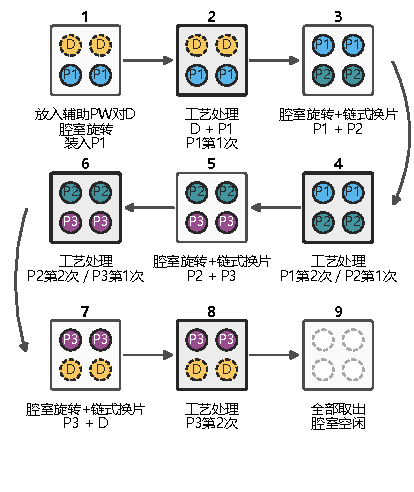
\includegraphics[width=0.93\linewidth]{fig_chain_cn_nature}
\caption{$2\times2$链式生产过程。辅助PW对D在链首与链尾保持腔室满片；产品晶圆随腔室旋转和链式换片参加相邻两个生产周期，每片产品晶圆完成两次工艺处理。}
\label{fig:chain-zh}
\end{figure}

\begin{figure}[t]
\centering
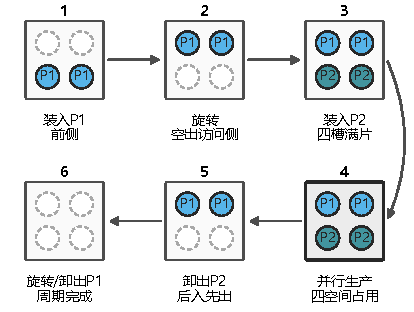
\includegraphics[width=\linewidth]{fig_parallel_cn_nature}
\caption{$4\times1$并行生产过程。两组PW对依次装入旋转腔，四个工位满片后同步执行一次工艺处理，再按后装先卸次序退出；末批不足时由辅助晶圆补位。}
\label{fig:parallel-zh}
\end{figure}

二元量$A_{pcq}$标识对$p$在腔室$c$的首次参加周期，派生量$Z_{pcq}$标识末次参加周期。取边界$X_{pc0}=X_{pc,Q_{\max}+1}=A_{pc,Q_{\max}+1}=0$，且$A_{pc1}=X_{pc1}$直接代入，有
\begin{equation}
\begin{aligned}
A_{pcq}&\ge X_{pcq}-X_{pc,q-1}, &A_{pcq}&\le X_{pcq},\\
A_{pcq}&\le1-X_{pc,q-1},\\
Z_{pcq}&=X_{pcq}-X_{pc,q+1}+A_{pc,q+1},\\
\sum_{c,q}X_{pcq}&=v_p+B_p^{\psi}, &\sum_{c,q}A_{pcq}&=v_p,\\
A^{\psi}_{pcq}&=X_{pcq}-Z_{pcq}, &Z^{\psi}_{pcq}&=X_{pcq}-A_{pcq},\\
\sum_pA^{\psi}_{pcq}&\le1, &\sum_pZ^{\psi}_{pcq}&\le1.
\end{aligned}
\label{eq:cycle-exposures-cn}
\end{equation}
首次进入标记的三条不等式使$A_{pcq}=X_{pcq}(1-X_{pc,q-1})$。因此，$Z_{pcq}$的差分定义恰为$X_{pcq}(1-X_{pc,q+1})$，且求和后自动得到$\sum_{c,q}Z_{pcq}=\sum_{c,q}A_{pcq}=v_p$，无需另加末次标记变量及其逻辑联结行。一个启用对仅有一次进入，且总占位为$v_p+B_p^{\psi}$，故其占位是长度为1或2的连续段。在此结构下，$A^{\psi}_{pcq}=X_{pcq}-Z_{pcq}=A_{pcq}\land B_p^{\psi}$、$Z^{\psi}_{pcq}=X_{pcq}-A_{pcq}=Z_{pcq}\land B_p^{\psi}$，可直接以差量代入。$4\times1$含产品对参加一个生产周期，$2\times2$含产品对参加同腔相邻两个生产周期。每个$2\times2$生产周期至多包含一个首次参加工艺处理的产品对和一个末次参加工艺处理的产品对，从而形成交替换片链。纯辅助补位对参加一个生产周期，清洁对参加一个清洁周期。

\noindent\textbf{加工时长与周期衔接。}
加工周期的起止时刻为$S_{cq},E_{cq}$，$d_m$为加工类型$m$的持续时间，$\overline T$为有效时间上界：
\begin{equation}
\begin{aligned}
E_{cq}-S_{cq}&=\sum_m d_mK_{cqm},\\
0\le S_{cq},E_{cq}&\le\overline T U_{cq},\\
S_{cq}&\ge E_{c,q-1}-M(1-U_{cq})\quad(q>1).
\end{aligned}
\label{eq:cycle-time-cn}
\end{equation}
该约束固定各类加工周期的持续时间，等待仅发生在动作之间。默认$4\times1$生产周期为180~s，$2\times2$生产周期为90~s，清洁周期为500~s；装卸与旋转的持续时间由相应事件单独计入。

\noindent\textbf{前后侧占位与旋转装卸。}
令二元量$f_{pcq}$选择加工时位于机械手访问前侧的对。由占位变化派生$\kappa_{cq}$和$\upsilon_{cq}$，分别标记保留上一周期的一个对和本周期后全部退出，取值均为0或1；它们无需作为独立选择：
\begin{equation}
\begin{aligned}
\kappa_{cq}&=\sum_p(X_{pcq}-A_{pcq}),\\
\upsilon_{cq}&=U_{cq}-\sum_p(X_{pcq}-Z_{pcq}),\\
f_{pcq}&\le A_{pcq},\qquad\sum_pf_{pcq}=U_{cq},\\
f_{pc,q-1}&\ge X_{pcq}-A_{pcq}\quad(q>1),\\
f_{pcq}&\ge B_p+K_{cq\psi}+X_{pcq}-2-\kappa_{cq}.
\end{aligned}
\label{eq:cycle-side-cn}
\end{equation}
新装对位于前侧；保留对经旋转转到后侧，且上一周期必须在前侧。新链首的$2\times2$产品对最后装入前侧。对$p$的装卸起止时刻记为$s_p^{\rm load},e_p^{\rm load},s_p^{\rm unload},e_p^{\rm unload}$，均沿用对应物理动作；腔室$c$周期$q$前后半周旋转的起止时刻记为$s_{cq}^{\rm rot\pm},e_{cq}^{\rm rot\pm}$，旋转动作记为$\mathrm{rot-}$和$\mathrm{rot+}$，分别由$U_{cq}$和$\upsilon_{cq}$启用，持续$r_c$。装载联结为
\begin{equation}
\begin{aligned}
X_{pcq}=1&\Rightarrow S_{cq}\ge e^{\rm load}_p,\quad
s^{\rm unload}_p\ge E_{cq},\\
A_{pcq}=1,\ f_{pcq}=0&\Rightarrow e^{\rm load}_p\le s^{\rm rot-}_{cq},\\
A_{pcq}=1,\ f_{pcq}=1&\Rightarrow s^{\rm load}_p\ge e^{\rm rot-}_{cq},\quad
S_{cq}=e^{\rm load}_p,\\
\kappa_{cq}=1&\Rightarrow s^{\rm rot-}_{cq}\ge E_{c,q-1}.
\end{aligned}
\label{eq:cycle-load-cn}
\end{equation}
全部退出时，周期后旋转在加工结束后开始。最后一次加工后的卸片关系为
\begin{equation}
\begin{aligned}
Z_{pcq}=1,\ f_{pcq}=1&\Rightarrow e^{\rm unload}_p\le s^{\rm rot+}_{cq},\\
Z_{pcq}=1,\ f_{pcq}=0,\ \upsilon_{cq}=1
&\Rightarrow s^{\rm unload}_p\ge e^{\rm rot+}_{cq},\\
Z_{pcq}=1,\ f_{pcq}=0,\ \upsilon_{cq}=0
&\Rightarrow s^{\rm unload}_p\ge e^{\rm rot-}_{c,q+1}.
\end{aligned}
\label{eq:cycle-unload-cn}
\end{equation}
若下一周期保留一个对，则新对的装载须等待被替换的后侧对完成卸载；若不保留，则下一周期装载须等待上一周期的两个对均卸完。上述条件均以指示约束或有效大常数线性化，并与VTR动作互斥共同约束换片。它们允许真实等待，不把等待并入固定旋转或取放时长。

\noindent\textbf{清洁触发与清洁动作链。}
整数$n_{cq}$记录周期$q$结束后自上次清洁以来的生产周期数。取候选尾部$U_{c,Q_{\max}+1}=0$，清洁计数与触发满足
\begin{equation}
\begin{aligned}
0\le n_{cq}&\le H U_{cq},\qquad n_{c0}=0,\\
K_{cq,\mathrm{cl}}=1&\Rightarrow n_{cq}=0,\\
U_{cq}=1,\ K_{cq,\mathrm{cl}}=0
&\Rightarrow n_{cq}=n_{c,q-1}+1,\quad n_{c,q-1}\le H-1,\\
K_{cq,\mathrm{cl}}=1&\Rightarrow 1\le n_{c,q-1}\le H,\\
n_{cq}&\le H-1+H U_{c,q+1},\\
K_{c1,\mathrm{cl}}&=0,\qquad
K_{cq,\mathrm{cl}}+K_{c,q-1,\mathrm{cl}}\le1\quad(q>1).
\end{aligned}
\label{eq:clean-counter-cn}
\end{equation}
每完成一个生产周期，计数增加1；清洁使计数归零。累计生产周期数达到$H$后必须清洁。累计1至$H-1$个生产周期后，可在满足满片、连续处理及资源约束的合法边界选择提前清洁，不要求后续生产采用特定模式。因此，相邻两次清洁之间包含1至$H$个生产周期。末段不足$H$时可选择不追加清洁，达到$H$时须追加末端清洁。由式~\eqref{eq:cycle-capacity-cn}和式~\eqref{eq:cycle-exposures-cn}，同一产品对必须连续参加两个$2\times2$生产周期，清洁不能插入其间。

清洁区段$e$由周期类型序列中的清洁边界导出。记$\mathcal V_c$为腔室$c$的生产任务集合（一个$4\times1$批次或一个$2\times2$生产周期），$a_{vce}=1$表示任务$v$属于区段$e$，$q^{\rm cl}_{ce}=1$表示该区段后有清洁；这些标记由周期结构联结，不另作清洁次数与区段划分决策。内部段以清洁结束，末段是否清洁由式~\eqref{eq:clean-counter-cn}确定。

任务$v$的起止事件记为$s_v,e_v$。区段$e$后的完整清洁任务起止事件记为$s^{\rm cl}_{ce},e^{\rm cl}_{ce}$，阶段起止事件记为$s^{\rm cl,\nu}_{ce},e^{\rm cl,\nu}_{ce}$，其中$\nu\in\{FL,BL,P,BU,FU\}$依次表示前装、后装、清洁处理、后卸、前卸。所有符号均引用相应物理事件，完整任务从前装开始到前卸结束。清洁前后关系及动作链为

\begin{equation}
\begin{aligned}
s_v&\ge e^{\rm cl}_{c,e-1}-M(1-a_{vce}) &&(e>1),\\
e_v&\le s^{\rm cl}_{ce}+M(1-a_{vce})+M(1-q^{\rm cl}_{ce}),\\
s^{\rm cl,BL}_{ce}&\ge e^{\rm cl,FL}_{ce}+r_c-M(1-q^{\rm cl}_{ce}),\\
s^{\rm cl,P}_{ce}&\ge e^{\rm cl,BL}_{ce}-M(1-q^{\rm cl}_{ce}),\\
s^{\rm cl,BU}_{ce}&\ge e^{\rm cl,P}_{ce}-M(1-q^{\rm cl}_{ce}),\\
s^{\rm cl,FU}_{ce}&\ge e^{\rm cl,BU}_{ce}+r_c-M(1-q^{\rm cl}_{ce}).
\end{aligned}
\label{eq:clean-time-cn}
\end{equation}
式~\eqref{eq:clean-time-cn}表示第$e$区段只能在前一次清洁完成后开始，并须在下一次清洁开始前结束。一次完整清洁任务包含两侧辅助晶圆装载、腔室旋转、清洁处理和反向卸载，其持续时间与资源占用共同约束VTR、旋转腔及四片辅助晶圆的可用时刻。

给定解后，$4\times1$批次侧位、$2\times2$产品对链位置及清洁区段均可由$X,A,Z,f$与周期类型恢复，无需再引入独立的位置变量。固定布局实验额外固定这些位置及服务次序，并采用仅末批补位规则：若后续同类批次存在，当前$4\times1$批次含两个产品对。联合模型允许在任一合法生产周期采用辅助补位。

\subsection{辅助晶圆复用与机械手、模块资源}
\label{sec:model-resource-cn}

晶圆路线和腔内加工规则还需满足实体资源的可用性。本节先为辅助晶圆借用任务选择实体身份，再分配机械手承片位置和模块槽位，最后通过互斥次序及驻留上限协调资源占用。

\noindent\textbf{辅助晶圆身份与循环复用。}
每个辅助晶圆位置对应借用需求$j=(p,r)$，其启用直接由$d_{pr}$表示，覆盖产品--辅助对、纯辅助补位对及清洁对。晶圆占位与周期选择联结供片与返回事件，实体辅助晶圆的占用区间从存储取出延续至归还完成。

各腔室可访问同一物理辅助库存，$\mathcal T_c$为共享库存对腔室$c$的可用身份集合；相同身份在不同腔室的借用也必须互斥。每个有效需求必须选择一片库存中的物理辅助晶圆：
\begin{equation}
\sum_{\tau\in\mathcal T_c}g_{j\tau}=d_{pr},
\qquad j=(p,r)\in\mathcal J_c^D.
\label{eq:dummy-assign-cn}
\end{equation}
式~\eqref{eq:dummy-assign-cn}表示有效需求恰好分配一次；辅助身份选择$g_{j\tau}$同时作为对应借用区间的资源占用标记；同一物理辅助晶圆的两次借用由共享资源互斥约束排序，因此只有在前一次卸载并返回存储区后才能复用。辅助身份选择决定哪些跨腔借用需要排序：即使产品配对、分腔和周期结构相同，不同辅助身份安排仍可改变两腔的并行生产区间。第~\ref{sec:joint-evidence-cn}节通过控制产品结构的对照量化这一影响。

\noindent\textbf{机械手承片与模块容量。}
ATR为双手机械手、VTR为四手机械手，旋转腔内部含四个晶圆工位，其承载能力分别为2片、4片和4片。同一时刻一台ATR或VTR只能执行一个协调搬运动作，同一旋转腔也只能执行一个统一的装卸、旋转或加工阶段。因此，在资源排序层面，ATR、VTR和每个旋转腔的执行机构均建模为一个独占动作资源（单位并发资源），其承片能力由逐片物理手分配与PW对占位关系共同表达，旋转腔的四工位容量由批次/链式占位状态保证。AL同样作为独占动作资源；上装载锁含U1、U2，下装载锁含L1、L2两个独立物理槽位；辅助晶圆库存则把每片晶圆视为一个可复用物理身份。资源分配以单个占用区间为单位：一次单片承片位置占用、一次辅助晶圆借用或一次执行机构互斥占用均选择一个允许的单元。以$o$表示该资源占用任务，有
\begin{equation}
\sum_{\ell\in\Gamma_o}h_{o\ell}=b_o.
\label{eq:slot-select-cn}
\end{equation}
式~\eqref{eq:slot-select-cn}表示每个启用的资源占用任务恰好选择一个允许的单元。$b_o\in\{0,1\}$表示任务是否启用，$h_{o\ell}\in\{0,1\}$表示是否选择单元$\ell$，$\Gamma_o$为允许的单元集合；未启用时所有$h_{o\ell}$均为零。两片晶圆成对搬运时，各自保留承片位置占用，动作同步由式~\eqref{eq:double-transfer-cn}协调。腔室四工位的满片条件由PW对占位关系保证，执行机构的互斥单元不代表承片数量。同一单元的占用区间不能重叠，由式~\eqref{eq:resource-order-cn}保证。当$\Gamma_o$仅含一个单元时，$h_{o\ell}=b_o$可直接代入，无需另设独立分配变量。辅助身份占用沿用$g_{j\tau}$，不重复引入另一套身份分配决策。

上装载锁槽位占用从ATR放片开始，持续至VTR取片完成并加上复位时间；下装载锁槽位占用从VTR放片开始，持续至ATR取片完成并加上复位时间。复位只限制该槽位的再次使用，可与取片后机械手的继续运输重叠。

VTR的四只手分为两只脏手$D_1,D_2$和两只洁净手$C_1,C_2$。对于未完成工艺处理的产品晶圆从上装载锁取片至放入腔室的承片任务，$\Gamma_o=\{D_1,D_2\}$；对于完成全部工艺处理的产品晶圆从腔室取片至放入下装载锁的承片任务，$\Gamma_o=\{C_1,C_2\}$。辅助晶圆的输入与返回均允许$\Gamma_o=\{D_1,D_2,C_1,C_2\}$。每项承片任务从取片动作开始持续至放片动作完成，式~\eqref{eq:slot-select-cn}选择的物理手在此区间内保持不变。相同手上的占用按式~\eqref{eq:resource-order-cn}互斥，其承片区间的换位间隔取零，机械手整体移动仍由动作资源的换位约束计入。因而脏手与洁净手各自最多承载两片，辅助晶圆同时竞争这两类空闲承片位置。$2\times2$产品在两个连续生产周期之间留在腔内，完成第二次工艺处理后才由洁净手取出。成对交换允许脏手持有待进行工艺处理的PW对、洁净手取出已完成工艺处理的PW对，但每片辅助晶圆也必须分配到当时空闲的具体手。

\noindent\textbf{资源互斥与地点相关换位。}
共享资源的先后关系分为给定次序和待定次序。操作先后弧及预设服务链中的操作按指定次序执行，其余冲突操作通过次序变量协调。固定布局的纯$4\times1$实验采用预设的对准和装载锁服务次序；当候选批次数不超过清洁阈值时，VTR也采用预设的批次装卸服务链。这些预设关系仅用于固定布局实验；联合模型由资源次序变量决定其余冲突动作的顺序。

若操作$o$和$o'$可能竞争资源$r$的同一槽位$\ell$，则
\begin{equation}
\begin{aligned}
s_{o'}&\ge e_o+\rho^r_{oo'}-M(1-y^r_{oo'})
-M(1-h_{o\ell})-M(1-h_{o'\ell}),\\
s_o&\ge e_{o'}+\rho^r_{o'o}-My^r_{oo'}
-M(1-h_{o\ell})-M(1-h_{o'\ell}).
\end{aligned}
\label{eq:resource-order-cn}
\end{equation}
式~\eqref{eq:resource-order-cn}表示当两项操作竞争同一资源占用单元时，二元变量$y^r_{oo'}$必须选择一种先后顺序；$\rho^r_{oo'}$同时计入机械手换位或设备复位时间。该式统一用于ATR、AL、上下装载锁、VTR、旋转腔和同一片辅助晶圆，因而既禁止机械手或腔室执行机构并发执行冲突动作，也禁止物理槽位或辅助晶圆在释放前被再次使用。

换位时间按地点对给定。对于腔室由$z_{pc}$决定的动作，按候选腔室组合启用相应移动时间间隔，而不预先固定其地点。例如，$o,o'$分别服务于对$p,p'$的互斥腔室动作且均启用时，有
\begin{equation}
\begin{aligned}
z_{pc}=z_{p'c'}=1,\ y^{\rm VTR}_{oo'}=1
\ \Rightarrow\ s_{o'}\ge e_o+\rho^{\rm VTR}_{cc'}.
\end{aligned}
\label{eq:location-travel-cn}
\end{equation}
其中$\rho^{\rm VTR}_{cc'}$是两个腔室间的给定移动时间；反向次序同理。对固定地点的动作，直接使用式~\eqref{eq:resource-order-cn}。

\noindent\textbf{驻留限制与时序可行性。}
对晶圆$w$进入和离开受限设备区段$r$的事件，有
\begin{equation}
0\le s_{\operatorname{out}(w,r)}-e_{\operatorname{in}(w,r)}
\le\overline R_{wr}.
\label{eq:residence-cn}
\end{equation}
式~\eqref{eq:residence-cn}表示晶圆在上装载锁、工艺腔室、下装载锁或受限制搬运区段中的物理停留时间不得超过上限，即驻留时间约束。装载锁的晶圆槽位占用在另一侧取片动作完成时结束，随后压力复位可与机械手继续运输并行；装载锁下一次不兼容操作须等待复位完成。

驻留上限保证的是相应区段的时间可行性，不要求同配方晶圆具有相同驻留时长。不同模式、不同区段的必要工艺与搬运时间也可能不同；若研究驻留一致性，应在同配方、同区段的可比晶圆之间定义离散程度，并直接评价或优化该指标。本文不以等待减少替代这一检验。

上述操作先后约束~\eqref{eq:precedence-cn}与资源排序约束~\eqref{eq:resource-order-cn}共同构成本文的死锁避免机制。对任一候选排程，把已激活操作作为节点，把操作先后关系和求解器选择的共享资源先后关系作为有向弧；若机械手、装载锁、旋转腔或辅助晶圆之间出现循环等待，则该操作--资源图中必然出现有向环。对于实际资源占用操作，沿环累加相应时间约束会产生正的持续时间或切换时间增量，从而要求某一操作的开始时刻严格晚于自身，违反时间可行性。因此，只有不存在循环等待、且所有晶圆都能沿完整路线从释放推进到返回的资源次序才能成为MILP可行解。结合装载锁槽位、旋转腔满片占位以及辅助晶圆返回后才能复用的显式建模，所建模动作中的循环等待通过时间可行性约束排除。

\subsection{完工时间优先的两阶段优化}
\label{sec:model-objective-cn}

前述约束共同定义联合可行域$\mathcal F$，$\xi$为其中全部保留变量构成的向量。第一阶段优化产品回片完工时间，第二阶段在保留第一阶段完工时间上界与主要离散结构的条件下优化等待与生产节拍。

\noindent\textbf{第一阶段：最小化产品回片完工时间。}
直接以回片动作结束时刻$e_{w,\mathrm{return}}$表示产品晶圆$w$回到原LP的时刻，第一阶段优化目标为
\begin{equation}
C_{\max}\ge e_{w,\mathrm{return}}\ (w\in\mathcal W),\qquad
\min_{\xi\in\mathcal F}C_{\max}.
\label{eq:primary-objective-cn}
\end{equation}
式~\eqref{eq:primary-objective-cn}表示最大完工时间按最后一片产品晶圆完成完整端到端路线并返回LP的时刻计算。若清洁位于两个生产段之间，其资源占用和前后关系会推迟后续产品回片，因而自然影响$C_{\max}$；若最后一次清洁之后不再有产品工艺处理，则该末端清洁仍保留在设备动作序列中，其完成时刻不直接作为$C_{\max}$的下界。末端清洁仍可能经共享VTR与其他腔室的产品回片竞争资源，因此其间接影响须由完整排程判定。WPH仅以产品回片的$C_{\max}$为分母。联合可行域$\mathcal F$由配对、分腔、周期占位和完整物理时序约束共同构成；固定布局实验另施加其布局与服务次序条件。

\noindent\textbf{第二阶段：限定优化范围并精修时序。}
设第一阶段获得当前最好可行解$\widehat\xi$，其产品完工时间为$\widehat C$。$\xi_d$为向量的第$d$个分量，带帽量在第二阶段作为常量。集合$\mathcal D_{\rm fix}$包含第二阶段固定的配对、分腔、周期占位、辅助身份、手分配、随行入片选择与资源次序。给定完工时间容差$\varepsilon_C$，第二阶段在原可行域上增加

\begin{equation}
\begin{gathered}
\xi_d=\widehat\xi_d\quad(d\in\mathcal D_{\rm fix}),\qquad
C_{\max}\le\widehat C+\varepsilon_C.
\end{gathered}
\label{eq:secondary-domain-cn}
\end{equation}

式~\eqref{eq:secondary-domain-cn}保留主要离散结构及产品完工时间上界，同地点原子取放同步选择与连续时刻继续参与优化。第一阶段即使尚未证明最优，也可用其当前最好可行解启动第二阶段。

令$\mathcal Q^w$为纳入评价的等待项索引集合，$\omega_\alpha$表示第$\alpha$项等待时长，即对应事件间隔扣除必要操作或移动时长后的非负余量。总等待直接以$\sum_\alpha\omega_\alpha$计入目标，实验表中的$L_{\rm sum}$仅为该求和结果的统计简写，不是独立变量；$L_{\max}$为最大单项等待的上界；并行发生的不同晶圆等待分别计入。$\omega_\alpha$是事件时刻的差分表达式，不再增加独立等待决策。
\begin{equation}
L_{\max}\ge\omega_\alpha\ge0,\qquad \alpha\in\mathcal Q^w.
\label{eq:secondary-wait-cn}
\end{equation}

节拍项直接使用周期开始时刻$S_{cq}$。集合$\mathcal I_h$包含同一腔室、同一$2\times2$链内连续三个生产周期的中心索引$(c,q)$，相邻两处边界均保留一个对，即$\kappa_{cq}=\kappa_{c,q+1}=1$，不跨清洁或链边界计算。第二阶段固定周期结构后，该集合随之确定。后一个开始间隔减去前一个间隔为$S_{c,q+1}-2S_{cq}+S_{c,q-1}$，以非负辅助量$v_{cq}$线性表示其绝对值上界，无需再引入区段时钟或差分变量：

\begin{equation}
\begin{aligned}
v_{cq}&\ge S_{c,q+1}-2S_{cq}+S_{c,q-1},\\
v_{cq}&\ge-S_{c,q+1}+2S_{cq}-S_{c,q-1}
\quad((c,q)\in\mathcal I_h).
\end{aligned}
\label{eq:secondary-rhythm-cn}
\end{equation}

若启用等待软上限$\bar\omega_\alpha$，以非负辅助量$\eta_\alpha$表示超额等待的上界：
\begin{equation}
\eta_\alpha\ge\omega_\alpha-\bar\omega_\alpha,\qquad
\eta_\alpha\ge0.
\label{eq:secondary-softwait-cn}
\end{equation}

将上述指标按非负权重$\lambda_1,\ldots,\lambda_4$组合，第二阶段目标为
\begin{equation}
\begin{aligned}
\min\ \ &\lambda_1\sum_{\alpha\in\mathcal Q^w}\omega_\alpha+\lambda_2L_{\max}\\
&+\lambda_3\sum_{(c,q)\in\mathcal I_h}v_{cq}
+\lambda_4\sum_{\alpha\in\mathcal Q^w}\eta_\alpha.
\end{aligned}
\label{eq:secondary-objective-cn}
\end{equation}

式~\eqref{eq:secondary-objective-cn}分别惩罚总等待、最大单项等待、相邻生产周期开始间隔的变化和软等待超额。正式实验采用$(\lambda_1,\lambda_2,\lambda_3)=(1,10,25)$、$\varepsilon_C=10^{-6}$；关闭软等待上限时不生成超额变量，也不计入对应惩罚项。

当对应权重严格为正且第二阶段达到最优时，上界辅助量取紧值：$L_{\max}=\max_\alpha\omega_\alpha$、$v_{cq}=|S_{c,q+1}-2S_{cq}+S_{c,q-1}|$及$\eta_\alpha=\max(0,\omega_\alpha-\bar\omega_\alpha)$。限时可行解中的辅助量可能存在松弛，因此各项指标均由实际事件时刻重新计算。节拍项衡量相邻生产周期开始间隔的变化，连续三个生产周期等间隔开始时该项为零。软等待上限允许超出并施加惩罚，驻留时间上限则作为硬约束执行。

\paragraph{等待、节拍与JIT的关系。} 式~\eqref{eq:secondary-wait-cn}减少事件之间扣除必要动作时长后的余量，式~\eqref{eq:secondary-rhythm-cn}减少同一链内相邻生产周期开始间隔的变化；两者均不直接最小化不同晶圆的驻留时间差。等间隔开始的周期仍可能因卸片等待不同而产生不同驻留时长。本文以减少等待和不规则衔接支持面向JIT的运行设计，不宣称已建立包含需求时刻、提前/延迟代价或驻留一致性目标的JIT调度模型。

\paragraph{等价实现与内存控制。}
实现中将固定时长动作的结束时刻直接代入为$s_o+d_ob_o$，将腔室周期结束时刻代入为开始时刻加所选类型的工艺时长，将周期启用标记代入为类型选择之和，并将等待量直接写为相邻事件间隔扣除必要时长。代入后保留原有非负性、时域上界及启用条件；最大等待和节拍绝对值上界仍使用辅助变量。由$f_{pcq}\le A_{pcq}$可将两者逻辑与直接写为$f_{pcq}$，其余前后侧派生差量也按定义代入。高复用的$d_{pr}$、$\kappa_{cq}$和$\upsilon_{cq}$则在实现中保留由等式唯一确定的缓存列，避免在大量约束中反复展开长表达式；这些缓存列不增加物理决策自由度。因此，正文的派生量数量不能直接当作求解器独立变量的数量。

进一步利用式~\eqref{eq:cycle-exposures-cn}中的连续占位结构，首次进入的前、后侧标记分别为$f_{pcq}$和$A_{pcq}-f_{pcq}$；末次退出的前、后侧标记分别为$f_{pcq}-(X_{pcq}-Z_{pcq})$和$X_{pcq}-f_{pcq}$。这是因为留至下一周期的对必须位于本周期前侧，而留自上一周期的对位于本周期后侧。上述标记不再逐一建立逻辑与变量。若输入中完全不存在某生产工艺，则相应的对模式和周期类型直接置0：每个生产周期必须包含产品对，故此常量传播不会删除任何可行排程。

机器人前缀载片计数也可进行条件代入。令$i,j$为按建模索引排列的一对动作，$o_{ij}=1$表示$i$先于$j$，$\Delta_j$为动作$j$的载片数增量。保留$2o_{ij}\le b_i+b_j$后，动作$i$之前来自$j$的贡献可由$\Delta_j(b_ib_j-o_{ij})$改写为$\Delta_j(b_j-o_{ij})$，无需再为$b_ib_j$建立辅助变量。该代入在$b_i=1$时恒等；$b_i=0$时前缀容量条件本来不启用。实现仅在$M\ge\sum_j|\Delta_j|+4$、从而未启用前缀的松弛行必然冗余时采用此改写，否则保留原逻辑与表示。动作之间的物理时序、移动时间与容量限制均保持不变。

对于具有$R$个可选单元的承片、槽位或辅助身份占用，为任务$i$定义由原分配变量唯一确定的整数编号$r_i=\sum_{\ell=1}^{R}\ell h_{i\ell}$；辅助晶圆使用相应的$g_{i\ell}$。未启用任务的编号为0。令$B$为事件时域上界$\overline T$加上0及上下装载锁复位时长的最大值，因而所有占用区间均满足$s_i\ge0$、$e_i\le B$；装载锁区间在此包含复位尾部。$B$由已有时间参数计算，不是新增输入或决策。将编号为$r_i$的区间平移$r_iB$，不同编号对应的时间段必然互不重叠，同编号则保持原时间关系。令$\epsilon_{ij}=2-b_i-b_j$，仅需一个二元次序选择$\theta_{ij}$即可表示互斥：
\begin{equation*}
\begin{aligned}
s_j+B(r_j-r_i)&\ge e_i-B(R+1)(1-\theta_{ij}+\epsilon_{ij}),\\
s_i-B(r_j-r_i)&\ge e_j-B(R+1)(\theta_{ij}+\epsilon_{ij}).
\end{aligned}
\end{equation*}
两任务均启用且编号相同时，平移项抵消，两式选择物理时间先后；编号不同时，按编号大小选择$\theta_{ij}$，即使原区间重叠也能满足两式。若有任务未启用，$B(R+1)$覆盖所有可能的端点差，条件行完全放松。故该表示与原同单元互斥关系具有相同的整数物理可行域，不再需要独立的“编号不同”标记及其联结行。允许单元集合互不相交的任务对不需要互斥行。编号列按等式一次计算，避免反复展开独热分配和。机器人动作的先后和换位约束仍单独保留。对于两腔且腔间移动时间相同的VTR动作，两个腔室编号之差的绝对值可由正、负两条线性下界表示，替代逐地点组合枚举；不满足该条件时沿用原枚举。这些改写不保证相同的LP松弛或搜索轨迹。

公共初始解的辅助变量补全只处理该物理排程已经选中的对与周期；固定结构的SPBS各层仍固定配对启用和周期类型，因此省略的候选始终未启用。补全结果随后提升到具有式~\eqref{eq:candidate-bounds-cn}完整容量的模型，检查全部原始约束并独立重放物理事件，才接受为初始解。正式主求解释放初始化固定关系，保留全部候选对与周期；初始解补全子问题的最优状态不作为完整问题的最优性证据。上述代入、资源互斥改写和初始化实现分别冻结源码与验证记录，不把旧代数表示下的运行时间直接归入新实现的算法性能比较。

\section{面向限时可行排程的求解框架}

算法的任务是在指定时间与内存预算内返回满足完整物理约束的排程，并继续改善可行目标与最优性界。设备参数改变后，可以对更新的确定性实例重新执行这一流程；本研究不据此假定旧排程在新参数下仍然可行。有限预算既来自复杂联合模型的计算负担，也服务于参数更新后的及时决策需求，但本文未测定真实设备的重调度截止时间。SPBS主要解决可行起点获取，时序精修改善已选结构的运行质量，学习割选择则作为可检验的搜索加速组件，而非模式选择结论成立的前提。

第2节给出晶圆、周期占位与完整路线联结的联合模型。求解框架包含结构化初始化、MILP搜索与时刻精修，同时用于固定结构特例和联合模型。固定结构基准用于训练与组件比较，联合模型采用冻结策略评价迁移后的搜索表现。原始可行性要求满片占位、双源晶圆路线和共享资源次序相互协调；对偶界的收紧则依赖作用于离散选择、连续时刻及其耦合关系的有效不等式。为分别利用这两类结构，本文以结构保持二元骨架（structure-preserving binary skeleton，SPBS）构造初始可行排程，并采用\method{}选择割平面。SPBS确定可行搜索的起点，\method{}决定候选割的保留数量与加入次序，SCIP负责有效割生成、可行性检验、上下界维护和最优性证明\citep{achterberg2009scip,bestuzheva2023scip}。

求解过程依次包括初始排程构造与验证、候选割生成、保留数量预测、有序割集搜索和角色次模补全，随后继续分支定界搜索。所选割均为原模型的有效不等式，且其系数保持不变；因此，割选择影响线性松弛的收紧过程，而不改变原整数可行域。

\subsection{SPBS初始解}

固定布局实验中的SPBS针对固定结构特例，沿用该特例的配对、腔室与清洁布局，并对尚可选择的资源次序和槽位构造初始骨架，再由受限MILP求解连续事件时刻。产品晶圆按输入顺序组成PW对；$4\times1$模式PW对依次映射到腔室、批次和前后侧位，$2\times2$模式PW对按腔室轮转分配到连续链位置。批次使用、末批、链位置和末位置等激活变量随之确定。清洁边界把每个腔室的生产序列分成若干区段：$4\times1$批次进入相应清洁区间，$2\times2$链在达到清洁阈值时以辅助晶圆结束当前区段，并在清洁后用新的链首辅助晶圆继续。上述生产任务、腔室归属及清洁边界由主模型布局确定；SPBS在此基础上协调辅助晶圆占用和连续时刻。

在资源层，SPBS根据同一工艺路线生成保守次序。ATR先安排各腔室的$4\times1$输入和返回，并在某腔室完成其末个满片批次后尽早衔接该腔室的首个$2\times2$PW对；随后按清洁区段推进链式输入与返回。装载锁槽位采用确定性的奇偶映射破除对称，VTR次序与ATR的批次推进及清洁动作保持一致。设第$q$个松弛层级中被固定的二元变量集合为$\mathcal F_q$，骨架值为$\widehat x_j$，受限可行性子问题通过式~\eqref{eq:spbs-fix-cn}施加这些选择。

\begin{equation}
\ell_j^{(q)}=u_j^{(q)}=\widehat x_j,\qquad j\in\mathcal F_q
\label{eq:spbs-fix-cn}
\end{equation}

此处$j$为MILP标量变量$x_j$的索引，$q\in\{1,\ldots,5\}$为初始化松弛层级；$\ell_j^{(q)},u_j^{(q)}$分别为该层级下变量$x_j$的下界和上界，$\widehat x_j$为骨架给定值。$\mathcal F_q$是固定变量索引集合，区别于第2节的联合可行域$\mathcal F$；此处$q$不表示加工周期。



式~\eqref{eq:spbs-fix-cn}表示SPBS只把当前层级的骨架选择固定为变量界；开始、完成、等待等连续变量，以及该层级未固定的资源次序保持自由。

SPBS采用逐级释放固定变量的可行性搜索。五个层级对应嵌套固定集合$\mathcal F_1\supseteq\mathcal F_2\supseteq\cdots\supseteq\mathcal F_5$；在骨架值不变时，释放固定条件使受限可行域逐级扩大。若某一级未在分配预算内得到可行解，则转入下一层级。
第一层级固定产品与批次分配、激活状态、清洁区段、装载锁槽位以及ATR、AL、LL和VTR的资源次序。第二层级释放VTR次序，第三层级进一步释放装载锁次序，第四层级释放其余资源次序而保留结构分配与槽位，第五层级仅保留产品分配、激活状态和清洁区段。对于32片及以上实例，可行性搜索从第四或第五层级开始；在严格等待上限下，还考虑不附加骨架固定条件的原可行域。

各层级均求解目标为零的受限可行性子问题，并在获得首个可行解后终止。求解采用可行性优先策略、强化启发式和快速预求解，子问题阶段不添加割平面。随后，在完整模型中保留所得排程的主要离散决策与连续时刻，并补全排程稳定性相关的辅助变量。通过原模型全部约束检验的排程作为主问题的初始可行解。主问题恢复SPBS临时收紧前的变量界，并保留原模型的布局等式；其搜索范围为给定布局下的完整可行域。实验中的SPBS初始排程预先离线构造，并与对应模型逐一核验；PDI的积分区间和主问题的计时范围均不包含初始排程的离线构造阶段。

联合模型的分层初始化从满足完整晶圆路线与物理手限制的初始排程出发，以产品完工时间为目标改善骨架。启用该初始化时，五层依次保留主要离散选择、释放VTR动作次序、释放装载锁次序、释放其余资源次序，最后仅保留配对及周期启用和类型等结构量；成对动作同步与连续时刻在各层均可调整。每层预算不超过初始化总预算的五分之一，并把当前最好完整可行赋值传递给后续层。进入联合主求解时解除全部临时固定条件，配对、分腔及资源次序重新参与优化。该初始化的完工时间改进目标区别于固定布局SPBS的零目标可行性搜索，构造成本与主求解预算分别计量。

\subsection{HEM基线与角色感知表示}

已有学习型割选择分别以强化学习、候选割排序和前瞻模仿处理通用MILP候选集\citep{tang2020cut,huang2022cutranking,paulus2022looking}。HEM进一步指出，割选择同时包含“选哪些、选多少、按什么顺序加入”三个相互关联的决策，并用高层数量策略与低层序列策略联合处理\citep{wang2023hem}。本文保留HEM的层次分解和pointer解码框架，把HEM的13维序列模型作为直接基线，在相同训练实例、预算、随机种子、候选上限和隐藏维数下比较输入表示、解码及选后补全。HEM后续已扩展为层次序列/集合模型\citep{wang2024hemset}；本文的HEM-13D对应2023年序列模型的受控复现。

HEM基线的13维候选向量依次包含目标平行度、割有效性、归一化支撑规模、整数支撑比例、归一化违反量、割系数的均值/最大值/最小值/标准差以及目标系数的四个对应统计量。这些量能够反映当前LP点处的割质量和数值尺度，但两个有效性相近的割仍可能分别作用于离散路线变量和连续时间变量。对本文模型而言，这一区别直接对应加工结构与资源组合的选择，以及既定组合下的时序收紧。

在HEM的13维通用特征上，本文按变量的数学属性把变量分为二元、一般整数、目标活跃连续、连续辅助和其他五类。割$i$在角色$g$上的系数质量为
\begin{equation}
p_{ig}=\frac{\sum_{j:x_j\in g}|a_{ij}|}{\sum_j|a_{ij}|+\varepsilon}.
\label{eq:role-mass-cn}
\end{equation}

在式~\eqref{eq:role-mass-cn}中，$i$索引候选割，$j$索引原MILP的标量变量$x_j$，$a_{ij}$为第$i$条割中$x_j$的系数；$g\in\mathcal G$索引变量角色，$p_{ig}$为割$i$在角色$g$上的绝对系数质量占比，$\varepsilon>0$为分母稳定常数。$\mathcal G$包含二元、一般整数、目标活跃连续、连续辅助和其他五类；$B,I,C_{\rm obj},C_{\rm aux}$为前四类的标签。这里的$a_{ij}$表示线性不等式系数，区别于第2节产品成员指示量$a_{wpr}$。


式~\eqref{eq:role-mass-cn}表示割系数绝对质量由各数学变量角色承担的比例。五个角色质量之外，新增特征还包括双边有限界变量质量、正系数质量、离散--连续耦合度$4(p_{iB}+p_{iI})(p_{iC_{\rm obj}}+p_{iC_{\rm aux}})$、最大非残余角色质量和归一化角色熵，共10维；与HEM特征合并后得到23维表示。角色划分仅取决于变量类型、目标系数和全局界，因此该表示对保持这些属性及割系数不变的变量重命名具有不变性。

HEM采用层次化“数量策略+有序子集策略”，其高层通过序列编码状态预测选割数量，低层采用LSTM编码器--解码器和pointer注意力逐项选择割\citep{wang2023hem,vinyals2015pointer}。本文在这一层次框架上构建角色感知割选择器：在候选进入LSTM之前引入角色感知分组门控编码，在pointer生成的有序序列之后加入角色次模补全，并在正式推理阶段采用宽度3的束搜索，以形成完整的RDMCT-HBS选择流程。


\subsection{角色感知编码与层次序列解码}

设第$t$次分离轮次保留的候选数为$m_t$。对候选割$i$，将23维输入写成$x_i=[x_i^{H};x_i^{R}]$，其中$x_i^{H}\in\mathbb R^{13}$为HEM通用特征，$x_i^{R}\in\mathbb R^{10}$为本文的角色特征。首先对完整向量作层归一化，再分别进行同维隐藏空间投影，并用完整23维信息生成逐维门控：
\begin{equation}
\begin{aligned}
\widetilde x_i&=\operatorname{LN}(x_i),\\
u_i^{H}&=W_H\widetilde x_i^{H}+b_H,\qquad
u_i^{R}=W_R\widetilde x_i^{R}+b_R,\\
g_i&=\sigma(W_g\widetilde x_i+b_g),\qquad
z_i=g_i\odot u_i^{H}+(1-g_i)\odot u_i^{R}.
\end{aligned}
\label{eq:gated-encoding-cn}
\end{equation}

下标$i$定位候选割；上标$H,R$分别标记HEM通用特征支路与角色特征支路。$\widetilde x_i$为$x_i$经层归一化$\operatorname{LN}$后的向量，$\widetilde x_i^{H},\widetilde x_i^{R}$为其两组分量；$u_i^{H},u_i^{R}$为投影后的128维支路向量，$g_i$为128维门值，$z_i$为融合结果。$W_H,W_R,W_g$分别为两支路投影和门控的权重矩阵，$b_H,b_R,b_g$为相应偏置；下标H、R、g表示网络部件。$\sigma(\cdot)$为sigmoid函数，$\odot$为逐元素乘法。上述权重和偏置在训练中学习、正式推理时固定；此处$\sigma$与第2节来源参数$\sigma$的含义不同。


式~\eqref{eq:gated-encoding-cn}中的$z_i\in\mathbb R^{128}$是候选割的融合嵌入。与直接把23维特征一次线性映射不同，两个投影支路分别保留通用LP质量和变量角色结构，门$g_i$再按候选自适应决定两类信息在每个隐藏维上的占比。因此，当两条割具有相近有效性但分别主要作用于离散路线变量和连续时间变量时，编码器仍可形成不同表示。该分组门控适配器是本文相对HEM输入表示的结构性改动。

融合后的候选按步骤1确定的可重复顺序输入单层LSTM：
\begin{equation}
(h_i,c_i)=\operatorname{LSTM}(z_i,h_{i-1},c_{i-1}),\qquad i=1,\ldots,m_t .
\label{eq:lstm-encoding-cn}
\end{equation}

$t$为分离轮次，$m_t$为该轮截断后的候选数，$i=1,\ldots,m_t$为编码顺序。$h_i,c_i$分别为处理候选$i$后的隐藏状态和记忆状态；$h_{i-1},c_{i-1}$为前一个编码位置的状态，二者均为128维向量。此处$c_i$为网络状态，不是工艺腔室编号$c$。


LSTM把单条割的局部特征变为包含候选池上下文的状态$h_i$；这些状态同时服务于高层保留数量策略和低层有序选择。本文采用128维隐藏状态对排序后的候选序列进行上下文化编码，使同一候选池得到确定的编码表示，该可重复性以相同候选行及返回索引为条件；有效性同分仍由原始索引打破，因此该序列表示以有效性排序及原始索引作为确定次序的依据。

在低层第$r$个解码步，解码器根据已选前缀形成的状态$d_r$和全部编码状态$h_i$先执行一次glimpse注意力，再计算pointer概率。记$M_{ri}$为掩码项：候选$i$若已在前缀中出现则$M_{ri}=-\infty$，否则为0，则
\begin{equation}
\begin{aligned}
a_{ri}&=v_g^\top\tanh(W_e h_i+W_d d_r)+M_{ri},\\
\alpha_{ri}&=\operatorname{softmax}_i(a_{ri}),\\
\bar h_r&=\sum_i\alpha_{ri}h_i,\\
b_{ri}&=v_p^\top\tanh(U_e h_i+U_g\bar h_r)+M_{ri},\\
P(i_r=i\mid i_{1:r-1},S_t)&=\operatorname{softmax}_i(b_{ri}).
\end{aligned}
\label{eq:pointer-decoding-cn}
\end{equation}

下标$r$为解码步，$i$为候选割编号；$a_{ri}$为glimpse注意力分数，$\alpha_{ri}$为对候选维$i$归一化后的注意力权重，$\bar h_r$为该步候选状态的加权摘要，$b_{ri}$为pointer选择分数。$W_e,W_d$分别投影编码状态与解码状态，$U_e,U_g$分别投影编码状态与glimpse摘要，$v_g,v_p$分别为两种评分的可训练向量；下标e、d、g、p标记网络部件。$M_{ri}$为候选掩码，区别于时间大常数$M$；$i_r$为第$r$步选中的割编号，$i_{1:r-1}$为此前有序前缀，$S_t$为第$t$轮编码后的候选状态。$P(\cdot\mid\cdot)$表示条件选择概率。


式~\eqref{eq:pointer-decoding-cn}说明pointer根据已选前缀计算后续割的条件概率：已选前缀通过解码器状态改变下一步分布，掩码保证无重复，glimpse先形成当前前缀下的候选池摘要，再由pointer产生下一条割的条件概率。该LSTM解码和pointer机制继承HEM/Pointer Network；本文改变的是其输入嵌入以及正式推理时如何搜索这一条件概率树。

训练阶段仍按策略分布随机采样以保留探索。正式推理阶段，束搜索在每一步维护$B=3$条部分序列。对父束$b=(i_1,\ldots,i_{r-1})$及其未选候选$j$，扩展分数为
\begin{equation}
L_r(b\oplus j)=L_{r-1}(b)+\log P(i_r=j\mid b,S_t),
\label{eq:beam-score-cn}
\end{equation}

$b$为一条父束前缀，$j$为尚未选择的候选割编号，$b\oplus j$表示在前缀末端追加$j$；$L_r$为长度$r$前缀的联合对数概率，初始空前缀满足$L_0=0$。$B$表示束宽，$\mathcal B_r$为第$r$步保留的前缀集合，二者均不表示生产批次。


随后从所有“父束$\times$候选”的扩展中保留$L_r$最大的3条。直到长度达到高层给出的$k_t$后取最高分序列。束搜索保留多个候选前缀，并以联合概率评价完整序列；随后，策略锚定的角色次模补全根据变量角色覆盖调整所选割集。

\subsection{从候选池到有序割集的逐步选择}

在第$t$次分离轮次中，算法按以下顺序工作。

\noindent\textbf{步骤1：建立候选池。} SCIP先按自身分离器生成并验证候选行$\mathcal C_t$。为控制候选状态的维数与评估成本，先按割有效性降序保留至多128个候选；有效性相同时按原始索引确定顺序，使输入池可重复。SCIP要求强制加入的割由求解器继续管理，不进入学习排序。

\noindent\textbf{步骤2：计算并编码状态。} 对候选池中的每一行提取13维HEM特征和10维角色特征，同时计算角色质量、主导角色和结构熵；随后按式~\eqref{eq:gated-encoding-cn}完成分组门控融合，并由式~\eqref{eq:lstm-encoding-cn}得到上下文化候选状态。编码后的候选集合构成$S_t$。

\noindent\textbf{步骤3：决定保留数量。} 高层策略输出经tanh限制在$[-1,1]$的动作，并映射为保留比例$\rho_t$；该比例再受全局上限0.2、SCIP本轮上限和最多16条割的数量上限共同约束，得到$k_t$。候选充足时至少保留两条，以保证每轮具有非空的候选子集。

\noindent\textbf{步骤4：逐个生成候选顺序。} 低层pointer策略在第$r$步根据$S_t$和已选前缀$i_{1:r-1}$计算剩余候选的概率，已选索引被掩码为负无穷，因而不会重复。高层数量和低层顺序的联合策略为

\begin{equation}
\pi_\theta(k_t,i_{1:k_t}\mid S_t)=\pi_\theta^H(k_t\mid S_t)
\prod_{r=1}^{k_t}\pi_\theta^L(i_r\mid S_t,i_{1:r-1}).
\label{eq:policy-cn}
\end{equation}

$\theta$为策略网络参数，$k_t$为第$t$轮保留的割数，$i_{1:k_t}$为长度$k_t$的有序割序列；$\pi_\theta^H$为高层数量策略，$\pi_\theta^L$为给定状态与前缀的低层选择策略。上标H、L在此分别表示高层、低层；$\rho_t$为高层输出映射得到的保留比例，下标$t$均表示分离轮次。


式~\eqref{eq:policy-cn}表示高层先给出本轮序列长度，低层再在这个长度内逐步选择不同候选；先选的割既影响随后可选集合，也通过解码器隐藏状态影响后续概率。

\noindent\textbf{步骤5：束搜索解码。} 训练时低层按概率随机采样以形成探索；测试时采用宽度3的束搜索。第$r$步把每条部分序列分别与所有未选候选连接，累加联合对数概率，再从“父束$\times$下一候选”的全部扩展中保留得分最高的3条。重复至长度$k_t$后输出最高得分序列。与逐步贪心相比，束搜索保留了早期次优但后续组合概率更高的前缀；这种有限宽神经组合搜索与神经组合优化中的束解码思想一致\citep{choo2022beam}。

\noindent\textbf{步骤6：角色次模补全。} 仅依赖联合概率的序列仍可能反复覆盖同一变量角色。算法保留pointer序列前$\lceil0.25k_t\rceil$条作为策略锚点，把其余策略顺序与按即时结构质量$q_i$排序的候选合并，并截取不超过$2k_t$条形成扩展池$\mathcal R_t$。对候选子集$S\subseteq\mathcal R_t$定义
\begin{equation}
\begin{aligned}
F_t(S)={}&\sum_{i\in S}(0.35q_i+0.20r_i)
+0.25\sum_{g\in\mathcal G}d_g\sqrt{\sum_{i\in S}p_{ig}}\\
&+\frac{0.20}{|\mathcal R_t|}\sum_{u\in\mathcal R_t}\max_{i\in S}s_{ui},
\end{aligned}
\label{eq:submodular-cn}
\end{equation}

式~\eqref{eq:submodular-cn}的$t$表示分离轮次，$S$为扩展池$\mathcal R_t$内已选割集合，$i$为已选割编号，$u$为池内被代表候选的编号，$g$为角色类别。$q_i$为割$i$的即时结构质量，$r_i$为其pointer顺序先验，$d_g$为角色$g$的需求占比，$s_{ui}$为候选$u$与$i$的截断相似度，$F_t(S)$为本轮集合$S$的代理效用。$A_t$为固定策略锚点集合，$U\subseteq\mathcal R_t\setminus A_t$为待补全子集；残余函数$f(U)$度量相对锚点的新增效用。此处$q_i,r_i,d_g$均为选割评价量，不是加工周期、物理资源或动作时长。


其中$r_i$为pointer顺序归一化先验，$d_g$为扩展池中角色$g$的需求占比，$s_{ui}$为候选$u$与$i$在通用质量和角色质量上的截断余弦相似度；$q_i$综合有效性、违反量、整数支撑、可识别角色比例、主导角色比例和结构熵。式~\eqref{eq:submodular-cn}的第一项保留即时质量和学习顺序，平方根覆盖项使重复加入同一角色的边际收益递减，最后一项使所选割代表扩展池的主要结构。算法从锚点集合出发，每一步计算所有未选候选的$F_t$边际增益并加入最大者，直至达到$k_t$。在权重、角色质量与截断相似度非负并取$F_t(\varnothing)=0$时，该模块项、凹覆盖项和设施位置项构成单调次模目标。固定锚点$A_t$及扩展池后，令$f(U)=F_t(A_t\cup U)-F_t(A_t)$，则基数约束下的贪心补全对该残余目标具有标准$1-1/e$近似性质\citep{nemhauser1978analysis}。该近似比度量固定扩展池内残余代理目标的覆盖质量；PDI与求解时间由计算实验评价。

最终有序割序列记为$S_t^\star$，上标$\star$标记本轮输出；所选$k_t$条割依次按锚点原顺序和贪心补全顺序加入当前LP。候选截断、状态编码、数量预测、序列解码和次模补全共同确定本轮用于收紧线性松弛的有序割集。

\begin{table}[!htbp]
\raggedright
\scriptsize
\setlength{\tabcolsep}{3pt}
\algorithmtitle{基于并行层次REINFORCE与束搜索的割平面选择算法}
\label{alg:cut-selection-cn}
\begin{tabular}{>{\raggedright\arraybackslash}p{0.92\columnwidth}}
\toprule
\textbf{算法步骤}\\
\midrule
\textbf{输入：}SCIP已验证候选行$\mathcal C_t$、高层策略$\pi_\theta^H$、低层pointer策略$\pi_\theta^L$、束宽$B=3$、本轮求解器割上限。\\
\textbf{输出：}加入当前LP的有序割集$S_t^\star=(i_1,\ldots,i_{k_t})$。\\
\textbf{1. 训练策略。}两个采样环境并行采集以$R=-\pdi$为终端回报的求解轨迹；采用独立EMA基线的层次REINFORCE和同步Adam更新高、低层策略。正式推理时固定参数。\\
\textbf{2. 形成候选池。}按有效性降序排列，同分时按原始索引排序，截取至多128行。\\
\textbf{3. 编码状态。}对每行计算13维HEM特征、10维角色特征及角色质量，经分组投影、sigmoid门控融合和LSTM编码得到候选状态。\\
\textbf{4. 确定保留数。}用$\pi_\theta^H$预测保留比例，并经0.2比例上限、SCIP上限和16条数量上限得到$k_t$。\\
\textbf{5. 初始化束。}以空序列和对数概率0初始化$\mathcal B_0$。\\
\textbf{6. 束搜索扩展。}对$r=1,\ldots,k_t$，由一次glimpse和pointer注意力得到掩码后的条件概率，将$\mathcal B_{r-1}$中的每个前缀与全部未选候选组合并累加对数概率。\\
\textbf{7. 束剪枝。}保留联合概率最高的3条父束--候选扩展得到$\mathcal B_r$；循环结束后取$\mathcal B_{k_t}$的首序列。\\
\textbf{8. 固定锚点。}保留首序列前$\lceil0.25k_t\rceil$条作为策略锚点$A_t$。\\
\textbf{9. 构造扩展池。}合并剩余pointer顺序与结构质量顺序，去重并截取至多$2k_t$条得到$\mathcal R_t$。\\
\textbf{10. 次模补全。}置$S\leftarrow A_t$；当$|S|<k_t$时，加入使$F_t(S\cup\{i\})-F_t(S)$最大的$i\in\mathcal R_t\setminus S$。\\
\textbf{11. 加入割平面。}将$S_t^\star$按锚点原顺序及补全选择顺序加入当前LP。\\
\bottomrule
\end{tabular}
\end{table}

\subsection{策略训练与精确求解}

一次SCIP限时求解构成一条求解轨迹，终端代价为该求解的PDI。当前策略在每个满足条件的割选择轮次中执行；训练以该轨迹首次有效候选集上的高层比例和低层随机序列为动作样本，并把完整求解的PDI反馈给两层策略。以$R=-\pdi$写成回报后，低层采用
\begin{equation}
\begin{aligned}
\widehat{\nabla_\theta J}
&=\frac1B\sum_{b=1}^B(R_b-\bar R_{\rm EMA})
\nabla_\theta\log\pi_\theta(\tau_b),\\
\bar R_{\rm EMA}&\leftarrow0.9\bar R_{\rm EMA}+0.1\bar R.
\end{aligned}
\label{eq:reinforce-cn}
\end{equation}

$J$为期望回报目标，$\nabla_\theta J$为其关于参数$\theta$的梯度，帽号表示样本估计。此处$B$为训练轨迹批量大小，$b=1,\ldots,B$为轨迹编号；$R_b$为轨迹$b$的回报，$\tau_b$为该轨迹首次有效候选集上的采样割序列，$\pi_\theta(\tau_b)$为相应策略概率。$\bar R$为本批回报均值，$\bar R_{\rm EMA}$为指数移动平均基线，下标EMA为方法标签。这里的$B,b,\tau_b$分别区别于束宽、父束和实体辅助晶圆身份。


式~\eqref{eq:reinforce-cn}给出带指数移动平均基线、以首个有效候选集的动作样本构造的批量策略梯度更新；$B$为轨迹批量大小，$\tau_b$为第$b$条轨迹首次有效候选集上的采样割序列。等价地最小化以PDI为代价的优势加权对数概率，并按序列长度平均低层对数概率，防止长割序列仅因项数更多而产生过大梯度。高层使用相同PDI代价和独立EMA基线，每两轮更新一次；两层梯度范数均截断为2。训练采用并行环境采样，并在每批样本收集完成后同步更新参数，形成并行层次REINFORCE训练过程\citep{williams1992reinforce,mnih2016a3c}。

训练集含五个实例和五个随机种子。每个种子使用两个采样环境，每个采样环境每轮完成四条采用30~s时间上限和1024~MB内存上限的求解轨迹，合计八条，训练60轮；低层和高层Adam初始学习率分别为$10^{-4}$和$5\times10^{-4}$，每10轮乘0.96。训练使用随机解码，正式推理使用宽度3的束搜索。每个配置--种子组合固定使用第60轮参数，不利用基准集或测试集选择模型参数；13维HEM、23维仅特征和23维完整方法分别训练，避免把不同输入含义或补全环境的权重混用。

\method{}只排序并选择SCIP已生成的有效割，SPBS只提交经完整模型检查的可行解；二者均不改变目标、约束、整数性或界逻辑。因此，学习模块影响的是搜索路径和限时内上下界收敛速度，而可行性和最优性仍具有与默认SCIP相同的含义。

\section{计算实验与结果分析}

实验围绕三个制造运行问题展开：满片与假片占用如何影响不同批量和清洁条件下的模式优选；保留产品完工时间后，等待与周期衔接能改善多少；在有限计算预算下能否及时获得有效排程。可行解获得率与产品完工时间回答排程可用性和批次效率，等待与节拍指标回答时序质量，gap与PDI用于解释求解过程。驻留一致性、对实时需求的JIT符合程度，以及含硬件偏差的闭环执行效果不在现有实测指标中。

\paragraph{清洁规则修订与证据边界。} 现行模型允许阈值前清洁、达到阈值必须清洁，并采用式~\eqref{eq:candidate-bounds-cn}的扩大候选容量。第~\ref{sec:optional-evidence-cn}节报告该规则下重新求解并核验的结果；此后的历史基准保留原规则、固定布局及原预算下的数值，均在标题中明确标记。历史最优性证书不直接移用于扩大后的可行域。所有新结论均以通过原模型检查和独立物理核验的排程为依据；无可行解超时和执行失败均不解释为不可行证明。



现行规则重验证采用含洁净手、脏手约束的联合模型。历史实验另分为同质手固定布局基准及分型承片联合模型，后者见第~\ref{sec:joint-evidence-cn}节。不同规则、布局、移动时间、承片条件和资源预算的结果分别报告，不合并进行算法性能比较。

\subsection{实验设计与指标}

历史实验在Windows~11工作站上完成，配置Intel Core Ultra~7 265KF处理器、32~GB内存及NVIDIA GeForce RTX~5060~Ti显卡（8~GB显存）；历史软件配置为SCIP~10.0.1、PySCIPOpt~6.1.0、PyTorch~2.11.0及Python~3.12.12。现行规则重验证使用同一工作站，逐批冻结模型、配置和策略检查点，以各批次运行记录为版本依据。各比较族的求解预算与初始化成本分别计量。

历史基准首先评价固定结构、双源配置$\sigma=1$下的模式与求解性能，第~\ref{sec:joint-evidence-cn}节另记录历史联合模型的算法对照、模式扫描、来源路线及参数扰动。历史实验包括960次SPBS配对运行、1500次等预算精修运行、300次析因运行、80次单因素扰动运行，以及各方法合计729次40--64片分布偏移运行。这些历史样本数不计入现行规则重验证的覆盖率。实验关注模式比较、等待与节拍、可行解获取、界收敛及规模效应；下述评价指标在各自匹配的比较族内使用。

各对照方法采用相同的MILP、SCIP版本、实例及随机种子，并在每个比较族内使用相同时间与内存限制。设$P(t)$为最小化问题在时刻$t$的原始界，即当前最优可行目标值；$D(t)$为对偶界，即搜索树给出的全局下界。进一步记$\Delta(t)=|P(t)-D(t)|$、$m(t)=\min\{|P(t)|,|D(t)|\}$和$M(t)=\max\{|P(t)|,|D(t)|\}$。当两界有限、同号且不相等时，按照SCIP的定义，终止相对原始--对偶间隙为：
\begin{equation}
G_{\rm end}=100\,\frac{\Delta(T)}{m(T)}.
\label{eq:terminal-gap-cn}
\end{equation}
若两界相等，SCIP令$G_{\rm end}=0$；若两界异号或有效界尚未同时获得，则返回$+\infty$。式~\eqref{eq:terminal-gap-cn}以两界绝对值中的较小者归一化，因此$G_{\rm end}$不以100\%为上限；超过100\%表示上下界绝对差大于两界绝对值中的较小者。

SCIP计算PDI时采用另一种有界归一化。记瞬时积分gap为
\begin{equation}
g_{\rm PDI}(t)=100\,\frac{\Delta(t)}{M(t)},\qquad
\pdi=\int_0^T g_{\rm PDI}(t)\,\mathrm dt.
\label{eq:pdi-gap-cn}
\end{equation}

本节$t\in[0,T]$为一次求解内经过的时间，$T$为PDI计时窗长度（s），区别于第2节生产周期容量上界$T$；$P(t),D(t)$分别为该时刻的原始上界、对偶下界，$\Delta(t)$为两界绝对差，$m(t),M(t)$为两界绝对值的较小值、较大值。$G_{\rm end}$为停止时的相对gap，$g_{\rm PDI}(t)$为积分使用的瞬时gap；下标end、PDI是指标标签，PDI的单位为百分数乘秒。


式~\eqref{eq:pdi-gap-cn}适用于有限同号且不相等的两界；两界相等时SCIP令$g_{\rm PDI}(t)=0$，其余情形令$g_{\rm PDI}(t)=100$。因此瞬时积分gap始终位于$[0,100]$，PDI越低表示越早缩小界差。PDI为0要求gap在几乎整个计时窗内为0；$G_{\rm end}=0$只表示运行结束时证明最优，而PDI还计入最优性证明之前的界差。两项指标均采用SCIP的定义与求解统计量\citep{achterberg2009scip,bestuzheva2023scip}。

历史基准以制造实例为推断单位：先在实例内聚合随机重复，再对配对实例差异计算非参数95\% bootstrap区间和Wilcoxon符号秩检验，并在预设分析族内作Holm校正；其中$p$表示$p$值。现行规则重验证仅报告配对观测及配置内汇总，未开展显著性推断。限时运行保留在各自汇总中，不将随机种子视为独立制造实例。





\subsection{阈值前可选清洁的重验证结果}
\label{sec:optional-evidence-cn}

\paragraph{协议与覆盖。} 本轮分别运行核心验证A、模式扫描B和组件消融C，每个配置采用求解器种子1、2、3，主求解预算为300~s；精修方法分配270~s主求解和30~s第二阶段。共享SPBS预计算预算为20~s，其构造成本另计。A、B的单进程内存限制为14000~MB，C为6000~MB，因此不跨批次合并性能指标。A串行执行；B包含早期串行单元及受内存门控的前台队列；C最多并行两个独立任务，同一GPU最多一个学习策略任务。所有比较先匹配配置和种子，再在配置内汇总三个种子。学习方法使用训练种子1、迭代60的冻结检查点，在新模型上作迁移评价，未在新规则下重新训练。

表~\ref{tab:optional-coverage-cn}给出完整计划单元的验收状态。A的两个固定结构单元原模型检查未通过，仍按失败保留；事后恢复的可行性检查不回填为本次成功观测。B的24次失败均为24片纯$2\times2$、$H=3$--10配置的共同初始解构造达到内存限制，不能解释为模式不可行。B的192个有效排程中，168次主求解因时间限制停止，24次因内存限制停止。C的216个单元均通过原模型和独立物理检查，主阶段均为时间受限。参数敏感性批次D在本次证据冻结时尚未完成，不纳入本节结论。

\begin{table}[!htbp]
\centering\small
\caption{现行规则重验证的计划单元与验收状态}
\label{tab:optional-coverage-cn}
\begin{tabular}{cccccc}\toprule
批次 & 计划 & 最优 & 受限可行 & 无解超时 & 失败\\\midrule
A：核心 & 126 & 4 & 108 & 12 & 2\\
B：模式 & 216 & 0 & 192 & 0 & 24\\
C：消融 & 216 & 0 & 216 & 0 & 0\\\bottomrule
\end{tabular}
\par\smallskip\footnotesize 最优性仅针对对应求解域；A的4个最优单元均为固定结构子问题。受限可行包括时间或内存限制；无解超时指未取得可行解。
\end{table}

\paragraph{初始化与结构对照。} A中四个匹配配置各运行三个种子：4片双源$H=3,10$、4片单源$H=3$及8片双源$H=3$。冷启动在12次300~s运行中均未获得可行解；串行初始解和SPBS初始解各12次均获得有效排程。SPBS对应完工时间依次为857、857、1491和2069~s，较串行初始解组的888、888、1520和2300~s降低3.49\%、3.49\%、1.91\%和10.04\%。这支持本组配置中初始化的作用，但不包含离线构造成本，不能解释为端到端加速。

在4片双源、$H=10$配置中，原固定结构的有效种子1、3均证明最优值为532~s；按腔室重分配辅助身份、保持产品配对、分腔和周期骨架的结构对照，在种子1、2、3分别取得566、410、410~s可行排程。种子3的410~s低于匹配固定结构的532~s，改善122~s（22.93\%），两腔生产重叠107~s。该存在性对照证明原辅助身份关系限制了可达目标；410~s仍为可行上界，既非完整联合问题最优值，也不证明三个种子均改善。完整联合搜索在相应300~s运行中仍保留857~s初始解，说明扩大结构空间并不保证限时搜索获得更好的排程。

\paragraph{同预算精修。} C包含4片和8片、$H=3,10$、单源和双源的八个混合配置，每个配置运行九种方法、三个种子。配对方法使用哈希一致的共同初始解。表~\ref{tab:optional-refine-cn}对比300~s直接求解与270~s主求解加30~s精修：总等待下降22.29\%--50.25\%，产品完工时间在$10^{-6}$~s级求解容差内保持不变。表内先按配置汇总三个种子；各配置的三个种子取得相同的表列指标，数值取整显示。最大单项等待并非每组均下降。

\begin{table}[!htbp]
\centering\footnotesize
\setlength{\tabcolsep}{2.3pt}
\caption{现行规则下八组配置的等预算精修（时间单位：s）}
\label{tab:optional-refine-cn}
\begin{tabular}{cccccc}\toprule
$N/H$ & 来源 & $C_{\max}$ & 总等待：前$\to$后 & 降幅（\%） & 最大等待\\\midrule
4/10 & 双源 & 857 & 681$\to$400 & 41.26 & 140$\to$71\\
4/10 & 单源 & 1491 & 1110$\to$600 & 45.95 & 124$\to$65\\
4/3 & 双源 & 857 & 681$\to$400 & 41.26 & 140$\to$71\\
4/3 & 单源 & 1491 & 1110$\to$600 & 45.95 & 124$\to$65\\
8/10 & 双源 & 1723 & 1135$\to$882 & 22.29 & 183$\to$183\\
8/10 & 单源 & 2985 & 2412$\to$1200 & 50.25 & 124$\to$65\\
8/3 & 双源 & 2069 & 864$\to$578 & 33.10 & 74$\to$74\\
8/3 & 单源 & 3933 & 3182$\to$1680 & 47.20 & 118$\to$65\\
\bottomrule\end{tabular}
\par\smallskip\footnotesize $C_{\max}$前后相同；最大等待列为精修前$\to$后。
\end{table}

这八个配置的排程均没有可形成三连生产周期的节拍评价中心，故节拍偏差记录为零不构成节拍改善证据。完整第二阶段目标、仅等待目标及二次惩罚目标取得相同的表列等待指标；本组样本不能区分节拍项或不同惩罚形式的作用。第二阶段子问题的最优状态也不代表第一阶段联合问题全局最优。

\paragraph{割选择与模式排序的证据边界。} C的六种300~s主求解方法均保留共同初始解的完工时间，八配置平均值均为1925.75~s，未观察到主要结构变化。表~\ref{tab:optional-cuts-cn}给出PDI和自定义割选择回调记录：学习方法仅在各自24次运行中的18次触发回调。完整方法与HEM的PDI存在描述性差异，但与贪心消融接近，且未改善主目标，因此不足以宣称学习策略或结构组件优于基线。三个精修变体的主阶段仅270~s，其PDI不与300~s方法直接比较。

\begin{table}[!htbp]
\centering\small
\caption{现行规则下300~s主阶段的组件对照}
\label{tab:optional-cuts-cn}
\begin{tabular}{cccc}\toprule
方法 & 平均PDI & 回调总次数 & 触发运行数\\\midrule
默认SCIP & 29513.46 & 0 & 0/24\\
HEM & 29728.40 & 57 & 18/24\\
完整方法 & 29317.35 & 64 & 18/24\\
仅特征 & 29375.97 & 65 & 18/24\\
贪心选择 & 29317.24 & 72 & 18/24\\
去结构组件 & 29490.91 & 64 & 18/24\\
\bottomrule\end{tabular}
\par\smallskip\footnotesize 每种方法为8配置$\times$3种子；PDI单位为\%$\cdot$s。回调仅指自定义选择器，默认SCIP的零值不表示没有求解器分离过程。
\end{table}

A中提前清洁与仅阈值清洁的12组匹配运行取得相同完工时间，尚未证明放宽清洁规则严格改善目标。B虽有3个有效排程采用阈值前清洁，但这只能证明相关选择被实际使用。在8片、16片的48组完整模式三元对照（配置与种子匹配）中，没有一种模式的可行上界低于所有对手的有效下界；24片又缺少纯$2\times2$的有效观测。因此，本轮既不确认全局模式优选，也不将缺失单元视为较差模式。

\FloatBarrier

\subsection{补充配对实验与规模验证}
\label{sec:supplement-evidence-cn}

补充实验使用独立冻结批次，不回填此前失败记录。固定结构对照、有效节拍配置及清洁规则对照分别验收12、48和96个排程，均采用每进程6000~MB、至多两个独立任务及每任务一个求解线程。直接求解预算为300~s，精修为270~s主阶段加30~s第二阶段；前两组共享SPBS预算20~s，清洁规则对照采用双方均可行的共同串行起点，SPBS预算为零。配置和求解器种子配对后，在每个制造配置内汇总三个种子，不将种子重复作为独立实例。下述数值均核对保存的模型及结果哈希，并重新执行独立物理检查。

\paragraph{固定结构的独立重复。} 在4片双源混合配置、$H=3,10$下，固定结构各三个种子均取得532~s的条件最优值；相应完整联合搜索在300~s内均保留857~s上界和39~s下界。这确认了所测试固定结构的目标值，也说明扩大可行域不保证限时搜索改善当前排程。固定结构的最优值不等于联合模型全局最优值。本次重复采用显式原始模型验解；早期批次的验解失败记录不因重复成功而改判，也不作为额外独立样本累计。

\paragraph{具有有效节拍中心的精修。} 新增8片纯$2\times2$配置，覆盖单源、双源及$H=5,10$。每个排程具有两个有效节拍中心；四种方法为直接求解、完整线性精修、仅等待精修及二次节拍惩罚精修，共48次运行。主阶段24次因时间限制停止、24次因内存限制停止，均保留合格可行解。表~\ref{tab:supplement-rhythm-cn}给出直接求解与完整线性精修的配置内汇总，三个种子的表列数值一致，时间取整显示。

\begin{table}[!htbp]
\centering\footnotesize
\setlength{\tabcolsep}{3pt}
\caption{有效节拍配置的配对精修结果（时间单位：s）}
\label{tab:supplement-rhythm-cn}
\begin{tabular}{ccccc}\toprule
来源/$H$ & $C_{\max}$ & 总等待：前$\to$后 & 降幅（\%） & 节拍偏差\\\midrule
单源/5 & 2335 & 1642$\to$960 & 41.53 & 62$\to$62\\
单源/10 & 2335 & 1642$\to$960 & 41.53 & 62$\to$62\\
双源/5 & 1241 & 1200$\to$498 & 58.50 & 54$\to$54\\
双源/10 & 1241 & 1200$\to$498 & 58.50 & 54$\to$54\\\bottomrule
\end{tabular}
\end{table}

产品完工时间在$10^{-6}$~s级容差内保持，最大单项等待分别由单源的121~s和双源的85~s降至65~s。这些结果支持具有有效节拍结构时仍可压缩等待，但节拍偏差变化未超过物理核验容差。仅等待与二次惩罚变体取得近似相同的指标；完整目标和二次目标相对仅等待目标的24组比较均未满足精修起始完整赋值一致的控制条件。因此，本组实验不能将等待下降归因于节拍惩罚项，也不能确认其独立收益或不同目标形式的优劣。

\paragraph{清洁规则的机制对照。} 新增4/6片、混合/纯$2\times2$、$H=3,4$及清洁时长100/500~s的16个配置，每个配置的两种规则采用三个相同种子和相同起点，共96次有效运行，主求解均因时间限制停止。48组配对的产品完工时间均相同，未出现可选清洁上界严格低于匹配旧规则下界的证据。该结果扩大了清洁规则对照的覆盖范围，但不支持阈值前清洁严格改善完工时间，也不证明两种规则的全局最优值相等。

\paragraph{16片可行排程与未完成的规模证明。} 在独立的13568~MB单进程协议下，16片双源的$H=3,10$与两种纯模式完成4次运行，主预算7200~s、离线SPBS预算300~s。$H=3$时纯$4\times1$、纯$2\times2$的上界分别为2633、3660~s，$H=10$时分别为2633、2639~s；四项下界均为39~s，两项因时间限制、两项因内存限制停止。它们是有效排程上界，不能标作最优甘特图，也不能据上界大小认证模式优选。不同资源协议的这些结果不与前述300~s对照合并进行性能推断。

24片模式补充、32片规模验证、完整析因和40--64片迁移批次均在参考准备阶段遇到资源或补全失败，尚未形成完整正式比较。另行实现的100片三组加工时长扩展仅得到通过物理重放的构造排程，首次完整模型尝试在记录构建完成前触发资源保护，尚无最优性证据；该扩展不计入本文现行模型的算法性能样本。失败不解释为物理不可行，未完成单元也不用于支持正面结论。

\FloatBarrier

\subsection{历史基准：清洁触发位置与批量驱动的工艺模式选择}

表~\ref{tab:gantt-config-zh}给出16片代表性甘特图对应的实验参数。两台旋转腔共享VTR，产品晶圆和辅助晶圆沿各自路线竞争机械手、装载锁和腔室空间；清洁计数、旋转及搬运时间均进入同一MILP。图示排程均通过SCIP原模型约束检验和独立时序核算，用于比较两种模式的资源占用与事件衔接。

表~\ref{tab:gantt-config-zh}中的数值定义历史固定布局实验配置。产品回片时间比较采用相同累计名义工艺时长：$4\times1$为一次180~s，$2\times2$为两次90~s。配方满足产品工艺要求作为比较前提，实验评价排程性能。

\begin{table*}[!htbp]
\centering
\scriptsize
\setlength{\tabcolsep}{2pt}
\caption{历史基准：固定布局清洁阈值实验与代表甘特图的参数（等总名义工艺时间场景）。}
\label{tab:gantt-config-zh}
\begin{tabular}{C{0.10\textwidth} C{0.29\textwidth} C{0.10\textwidth} C{0.29\textwidth}}
\toprule
类别 & 参数与取值 & 类别 & 参数与取值\\
\midrule
旋转腔 & CH1、CH2，两台旋转腔共享VTR，每腔4个工位 & 工艺时长 & $4\times1$为180~s；$2\times2$为90+90~s\\
清洁 & 相邻清洁间最多$H=3$--10个生产周期；纯辅助晶圆清洁500~s & 腔室动作 & 旋转180$^\circ$为2~s；相邻腔室动作间隔1~s\\
ATR & 1台双手机械手，容量2；装/卸4~s，完整带片搬运11~s & VTR & 1台四手机械手，容量4；带片搬运4~s，空载换位4~s\\
ATR细节 & LL--LP空载返回6~s；AL处PW对交换8~s & AL & 容量1；每片最小对准占用20~s\\
装载锁 & LLupper每槽抽气/复位30~s，LLlower每槽放气/复位25~s & LL容量 & upper和lower各含2个独立槽位\\
晶圆源 & LP1--LP4，每个容量25片 & 辅助晶圆 & 可复用8片，每腔4片；存储区容量10片\\
批次与模型 & 产品基本批量4片；13个路线步骤 & 腔室容量界 & 每台PM最多15个$4\times1$批次槽\\
模型上界 & Big-$M=10000$；模块和机械手驻留上界均为10000~s & 等待设置 & 可避免等待硬上限取0，表示关闭该可选限制\\
求解目标 & 产品回片完工时间与等待精修 & 策略 & 固定训练种子1、第60轮、23维特征\\
解码与割池 & 束宽3；候选割池128，单轮最多选16条 & 求解器 & SCIP随机种子1；采用可用且通过验解的初始排程\\
求解与选图 & 产品回片目标；模式比较采用完工时间界；甘特图采用等待精修后的排程 & 排程验证 & 所有排程均通过原模型及独立验解\\
\bottomrule
\end{tabular}
\end{table*}


多空间CT的稳态研究通常以周期或吞吐率评价设备效率\citep{gu2024multifinger}。本文针对有限批次，以最后一片产品晶圆返回LP的时刻定义$C_{\max}$，并以$\mathrm{WPH}=3600|\mathcal W|/C_{\max}$表示等效批次产出率。纯$4\times1$每片工艺时长为180~s，纯$2\times2$每片工艺时长为90+90~s，1:1混合模式按晶圆所属模式使用相应配方。$H$为每腔相邻清洁间满片生产周期数的上限，$4\times1$批次计1次，$2\times2$的每个生产周期计1次；清洁不计入生产周期，本组历史固定布局实验仅在为后续完整$2\times2$链预留容量时于$H-1$后提前清洁。该固定布局生成器按周期上限和完整链边界构造生产区段，并计入500~s清洁及其辅助晶圆装卸、旋转和搬运。

表~\ref{tab:mode-extended-zh}给出$H=3$和10的模式比较，表~\ref{tab:clean-crossover-zh}汇总$H=3$--10的逐点结果。其中$H=4$--9实验包含36个配置，训练与求解器种子均为1，每例主求解上限14400~s，关闭第二阶段；36个排程均通过独立验解，其中35个证明最优。16片、$H=5$、纯$2\times2$在该预算内获得907~s可行解；以此为初始排程，对同一实例追加28800~s独立求解后，可行上界降至898~s，下界为694~s，终止gap为29.39\%。新排程通过主模型复验与4~s交换检查。该延长预算实验用于确定模式比较中的可行上界，其计算时间不计入固定预算的算法性能比较。清洁未激活时，16片纯$2\times2$在$H=6$--10下生成相同的MILP，最优完工时间均为898~s。

\begin{table*}[!htbp]
\centering
\scriptsize
\setlength{\tabcolsep}{4pt}
\caption{历史基准：相同累计名义工艺时长下的清洁端点比较。清洁总次数为两台腔室的内部与末端清洁次数之和。 $\dagger$表示经验证的完工时间上界；相应WPH按该完工时间计算。}
\label{tab:mode-extended-zh}
\begin{tabular}{cccccc}
\toprule
批次（片） & $H$ & 模式 & 清洁总次数 & $C_{\max}$（s） & WPH（片/h）\\
\midrule
8 & 10 & 纯$4\times1$ & 0 & 610 & 47.21\\
8 & 10 & 纯$2\times2$ & 0 & \textbf{578} & \textbf{49.83}\\
8 & 10 & 4:4混合模式 & 0 & 654 & 44.04\\
8 & 3 & 纯$4\times1$ & 0 & 610 & 47.21\\
8 & 3 & 纯$2\times2$ & 2 & \textbf{578} & \textbf{49.83}\\
8 & 3 & 4:4混合模式 & 1 & 654 & 44.04\\
\midrule
16 & 10 & 纯$4\times1$ & 0 & 944 & 61.02\\
16 & 10 & 纯$2\times2$ & 0 & \textbf{898} & \textbf{64.14}\\
16 & 10 & 8:8混合模式 & 0 & 939 & 61.34\\
16 & 3 & 纯$4\times1$ & 0 & \textbf{944} & \textbf{61.02}\\
16 & 3 & 纯$2\times2$ & 4 & 1402 & 41.08\\
16 & 3 & 8:8混合模式 & 2 & 1530 & 37.65\\
\midrule
24 & 10 & 纯$4\times1$ & 0 & 1268 & 68.14\\
24 & 10 & 纯$2\times2$ & 0 & $\mathbf{1237}^{\dagger}$ & \textbf{69.85}\\
24 & 10 & 12:12混合模式 & 0 & 1250 & 69.12\\
24 & 3 & 纯$4\times1$ & 2 & \textbf{1268} & \textbf{68.14}\\
24 & 3 & 纯$2\times2$ & 6 & $2220^{\dagger}$ & 38.92\\
24 & 3 & 12:12混合模式 & 4 & $2324^{\dagger}$ & 37.18\\
\bottomrule
\end{tabular}
\end{table*}

\begin{table*}[tp]
\centering
\scriptsize
\setlength{\tabcolsep}{3pt}
\caption{历史基准：给定PW对布局下，8、16和24片批次在$H=3$--10下的三模式完工时间、清洁次数与优选模式。时间单位为s。}
\label{tab:clean-crossover-zh}
\begin{tabular}{cccccccccc}
\toprule
\multirow{2}{*}{批次（片）} & \multirow{2}{*}{$H$} & \multicolumn{3}{c}{$C_{\max}$（s）} & \multirow{2}{*}{$\Delta C_{\max}$（s）} & \multicolumn{3}{c}{清洁总次数} & \multirow{2}{*}{优选模式}\\
\cmidrule(lr){3-5}\cmidrule(lr){7-9}
 & & 纯$4\times1$ & 纯$2\times2$ & 1:1混合模式 & & 纯$4\times1$ & 纯$2\times2$ & 1:1混合模式 & \\
\midrule
8 & 3 & 610 & 578 & 654 & -32 & 0 & 2 & 1 & 纯$2\times2$\\
8 & 4 & 610 & 578 & 654 & -32 & 0 & 0 & 0 & 纯$2\times2$\\
8 & 5 & 610 & 578 & 654 & -32 & 0 & 0 & 0 & 纯$2\times2$\\
8 & 6 & 610 & 578 & 654 & -32 & 0 & 0 & 0 & 纯$2\times2$\\
8 & 7 & 610 & 578 & 654 & -32 & 0 & 0 & 0 & 纯$2\times2$\\
8 & 8 & 610 & 578 & 654 & -32 & 0 & 0 & 0 & 纯$2\times2$\\
8 & 9 & 610 & 578 & 654 & -32 & 0 & 0 & 0 & 纯$2\times2$\\
8 & 10 & 610 & 578 & 654 & -32 & 0 & 0 & 0 & 纯$2\times2$\\
\midrule
16 & 3 & 944 & 1402 & 1530 & 458 & 0 & 4 & 2 & 纯$4\times1$\\
16 & 4 & 944 & 1470 & 939 & 526 & 0 & 2 & 2 & 1:1混合模式\\
16 & 5 & 944 & 898$^{\dagger}$ & 939 & -46 & 0 & 2 & 0 & 纯$2\times2$\\
16 & 6 & 944 & 898 & 939 & -46 & 0 & 0 & 0 & 纯$2\times2$\\
16 & 7 & 944 & 898 & 939 & -46 & 0 & 0 & 0 & 纯$2\times2$\\
16 & 8 & 944 & 898 & 939 & -46 & 0 & 0 & 0 & 纯$2\times2$\\
16 & 9 & 944 & 898 & 939 & -46 & 0 & 0 & 0 & 纯$2\times2$\\
16 & 10 & 944 & 898 & 939 & -46 & 0 & 0 & 0 & 纯$2\times2$\\
\midrule
24 & 3 & 1268 & 2220$^{\dagger}$ & 2324$^{\dagger}$ & 952 & 2 & 6 & 4 & 纯$4\times1$\\
24 & 4 & 1268 & 2928$^{\dagger}$ & 1827$^{\dagger}$ & 1660 & 0 & 4 & 2 & 纯$4\times1$\\
24 & 5 & 1268 & 1769$^{\dagger}$ & 1796 & 501 & 0 & 2 & 2 & 纯$4\times1$\\
24 & 6 & 1268 & 1880$^{\dagger}$ & 1263$^{\dagger}$ & 612 & 0 & 2 & 1 & 1:1混合模式\\
24 & 7 & 1268 & 1237$^{\dagger}$ & 1250 & -31 & 0 & 2 & 0 & 纯$2\times2$\\
24 & 8 & 1268 & 1237$^{\dagger}$ & 1250 & -31 & 0 & 0 & 0 & 纯$2\times2$\\
24 & 9 & 1268 & 1237$^{\dagger}$ & 1250 & -31 & 0 & 0 & 0 & 纯$2\times2$\\
24 & 10 & 1268 & 1237$^{\dagger}$ & 1250 & -31 & 0 & 0 & 0 & 纯$2\times2$\\
\bottomrule
\end{tabular}
\par\smallskip
\parbox{0.95\textwidth}{\footnotesize 清洁总次数为两台腔室内部与末端清洁之和。$\dagger$表示可行上界，其余完工时间已证明最优。$\Delta C_{\max}$为表列纯$2\times2$与纯$4\times1$时间之差。优选模式由最优值比较或可行上界低于竞争模式下界确定。}
\end{table*}

8片批次在$H=3$--10下的三模式完工时间分别保持610、578和654~s，纯$2\times2$较纯$4\times1$缩短5.25\%。$H=3$时纯$2\times2$与混合模式分别产生2次和1次末端清洁；$H\ge4$时均无清洁。该批量未形成内部清洁，模式排序在所测清洁阈值内保持一致。

16片批次的优选模式随清洁阈值变化。$H=3$时，纯$2\times2$和混合模式各含2次内部清洁，纯$4\times1$以944~s最优。$H=4$时，纯$2\times2$仍含2次内部清洁，混合模式仅含2次末端清洁，以939~s优于纯$4\times1$的944~s。$H=5$时，纯$2\times2$只产生2次末端清洁，其898~s可行排程优于另外两种模式的最优值，纯模式优先顺序由$H=4$的$4\times1$切换为$H=5$的$2\times2$。$H=6$--10时三模式均无清洁，纯$2\times2$以898~s最优，较纯$4\times1$和混合模式分别缩短4.87\%和4.37\%。

这一变化由完整链分段和清洁位置共同驱动。16片纯$2\times2$每腔包含4个产品PW对；$H=3$按2+2个PW对分段，$H=4$按3+1分段，$H\ge5$可形成一条完整链。因此，$H=3$和4虽然内部清洁数相同，仍具有不同的供片与回片次序；$H=4$的1470~s对应后一分段布局。模式选择需要同时匹配批量、配方构成和允许的完整链长度。实验采用随$H$重构的预设完整链布局，因此表中比较反映清洁阈值与链布局的联合效应。

24片批次的扩展实验覆盖$H=3$--6及三种预设模式，每个配置的主求解预算为7200~s。纯$4\times1$在四个清洁阈值下的最优完工时间均为1268~s。$H=4$时，纯$2\times2$与混合模式的求解下界分别为1342和1774~s；$H=5$时，纯$2\times2$的下界为1440~s，混合模式的最优值为1796~s，因此这两个清洁阈值均由纯$4\times1$优选。$H=6$时，混合模式取得1263~s可行排程，低于纯$4\times1$的最优值1268~s及纯$2\times2$的下界1440~s，确定了混合模式的模式优势；混合模式自身的终止gap为10.40\%。$H=3$的纯$2\times2$配置经28800~s独立求解，得到2220~s可行排程、2082~s下界和6.63\%终止gap。该排程通过主模型复验及4~s交换检查；其下界与混合模式下界2302~s均高于纯$4\times1$的最优值1268~s，因而$H=3$也由纯$4\times1$优选。延长预算的求解用于模式排序判定，运行时间不纳入原固定预算的算法比较。由此，24片批次在$H=3$--5时优选纯$4\times1$，在$H=6$时优选1:1混合模式。与16片结果相比，24片批次在$H=5$时的优选模式由纯$2\times2$变为纯$4\times1$，说明清洁阈值的模式选择效应取决于批量与完整链布局。

24片$H=7$--10的12个配置均获得通过验解的排程。对$H=10$混合模式的独立求解在28800~s预算内证明最优完工时间为1250~s；$H=7$--10的混合模式MILP的目标、约束与变量界完全相同，因此四个清洁阈值对应相同的最优完工时间。纯$2\times2$在$H=8$--10下具有1237~s可行排程；将其生产事件时序迁移至$H=7$模型，并安排两次末端清洁后，同样得到经原模型复验的1237~s排程。纯$2\times2$在$H=7$及$H=8$--10下的有效界区间分别为$[712,1237]$和$[842,1237]$~s。其可行上界均低于混合模式的1250~s与纯$4\times1$的1268~s最优值，因此$H=7$--10均优选纯$2\times2$，所构造排程较两种竞争模式分别缩短1.04\%和2.44\%。延长预算求解与排程迁移用于模式判定，其计算时间独立于固定预算的算法比较。

四张资源甘特图均采用16片批次，分别展示$H=10$和3的两种纯模式。各图横轴截至最后一片产品返回时刻$C_{\max}$；纯$4\times1$每次工艺处理180~s，纯$2\times2$每次工艺处理90~s。为分析最短完工时间排程的等待分布，$H=10$纯$2\times2$在保持$C_{\max}\le898+10^{-6}$~s的条件下进一步最小化路线总等待，并允许调整资源次序；所得最优路线总等待为492~s。路线等待按每片晶圆六个相邻工序间隔累计，其中AL成对协调占448~s、工艺处理完成后卸片前等待占36~s、下装载锁回片前等待占8~s。该路线指标统计工序间等待，腔室内相邻生产周期之间的间隔另行计量。

图中腔室泳道将交换动作与等待分开绘制：灰色交换块按实际动作起止时刻绘制，额外等待以浅粉色表示。此处的相邻生产周期间隔指前一周期结束至后一周期开始的时间，由交换前等待与交换过程共同构成。四指VTR的合并交换耗时4~s；拆分交换包含4~s卸片、至少4~s空载换位及4~s装片，并允许在卸片与装片之间协调其他晶圆动作。图~\ref{fig:gantt-cleanH10-22-zh}中CH1首次相邻生产周期间隔为63~s，其中59~s为交换前等待，4~s为合并交换。该排程中，下一产品PW对W5/W6在299~s进入上装载锁，329~s完成真空侧准备；CH1于270~s结束前一周期后等待至329~s，再执行329--333~s的合并交换。$H=3$的短链排程中，多数相邻周期采用连续4~s合并交换；CH1第五、六周期之间包含1106--1108~s和1112--1116~s两段等待，以及1108--1112~s卸片和1116--1120~s装片。末次工艺处理在装片完成的1120~s立即开始，至1210~s结束。两种排程均保持每次工艺处理90~s。进一步在同一$H=10$模型中将两个腔室全部8个相邻生产周期间隔限制为4~s，得到经独立验解的最优完工时间960~s，比898~s增加62~s（6.90\%）。连续交换压缩了局部生产周期间隔，同时约束了共享资源的供回片次序；在该有限批次下，允许局部等待获得更短的整批完工时间。

\begin{figure}[!t]
\centering
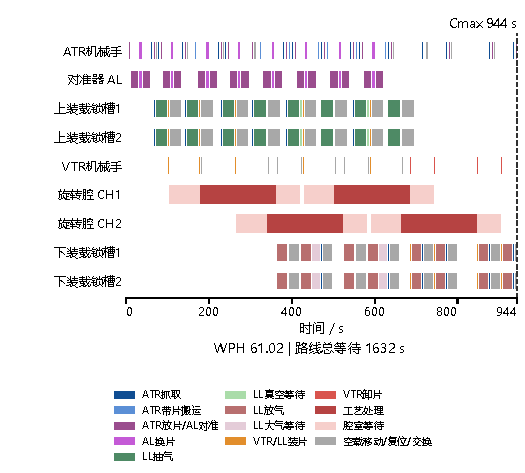
\includegraphics[width=\linewidth]{fig_resource_gantt_cleanH10_w16_41_cn_nature}
\caption{历史基准：同质手固定布局基准：$H=10$时16片纯$4\times1$排程。无清洁，$C_{\max}=944$~s，WPH为61.02片/h，路线累计等待为1632~s。}
\label{fig:gantt-cleanH10-41-zh}
\end{figure}

\begin{figure}[!t]
\centering
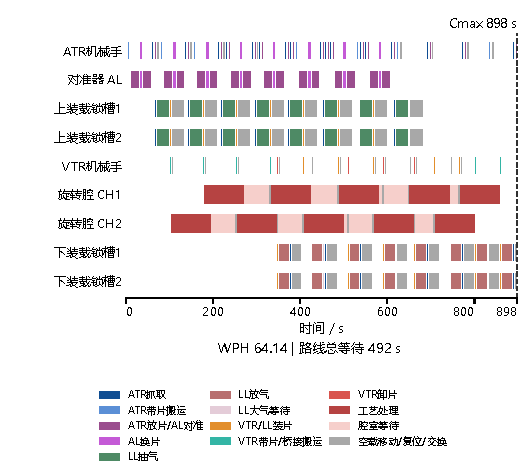
\includegraphics[width=\linewidth]{fig_resource_gantt_cleanH10_w16_22_cn_nature}
\caption{历史基准：同质手固定布局基准：$H=10$时16片纯$2\times2$的等待精修排程。无清洁，$C_{\max}=898$~s，WPH为64.14片/h；在该完工时间约束下，路线累计等待最小值为492~s。腔室泳道中灰色表示4~s交换动作，浅粉色表示等待。}
\label{fig:gantt-cleanH10-22-zh}
\end{figure}

\begin{figure}[!t]
\centering
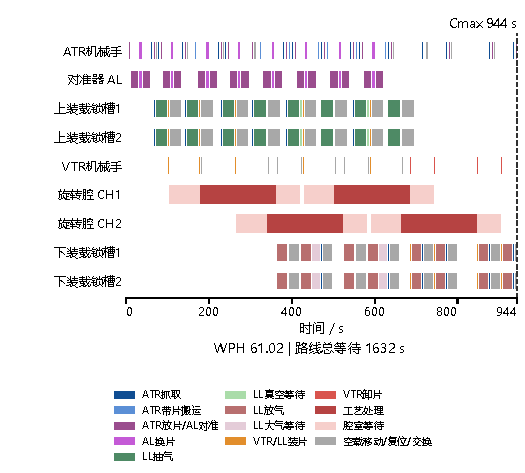
\includegraphics[width=\linewidth]{fig_resource_gantt_cleanH3_w16_41_cn_nature}
\caption{历史基准：同质手固定布局基准：$H=3$时16片纯$4\times1$排程。$C_{\max}=944$~s，WPH为61.02片/h，路线累计等待为1632~s。}
\label{fig:gantt-cleanH3-41-zh}
\end{figure}

\begin{figure}[!t]
\centering
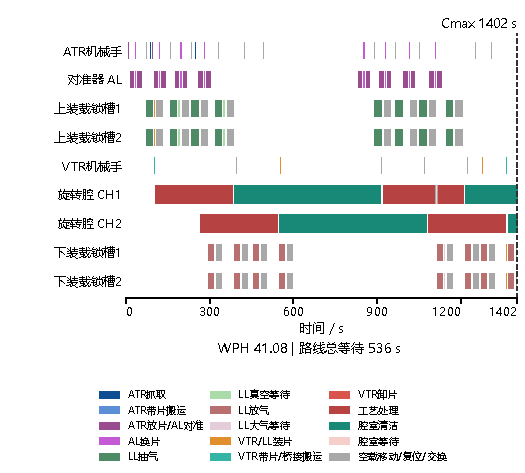
\includegraphics[width=\linewidth]{fig_resource_gantt_cleanH3_w16_22_cn_nature}
\caption{历史基准：同质手固定布局基准：$H=3$时16片纯$2\times2$排程。包含2次内部清洁和2次末端清洁；图示时域截至产品回片，$C_{\max}=1402$~s，WPH为41.08片/h，路线累计等待为536~s；腔室泳道中交换动作与等待分别绘制。}
\label{fig:gantt-cleanH3-22-zh}
\end{figure}


\subsection{历史基准：等预算下的等待与节拍精修}

等待时间约束会进一步影响制造系统的产出和控制表现\citep{lee2018waiting}。同为600~s总预算时，完整两阶段工作流采用540~s主求解加至多60~s精修，单阶段对照将600~s全部用于主求解。图~\ref{fig:workflow-zh-new}显示，两阶段工作流的路线总等待、最大等待、节拍变异系数和节拍偏差分别降低51.91\%、68.89\%、39.70\%和94.05\%，四项实例级配对差异经Holm校正后均显著，表明两阶段工作流能够在相同总预算下明显改善排程等待与节拍质量。

二次目标对照与完整线性精修均使用540+至多60~s。线性精修的节拍偏差为22.04，较二次目标的60.18降低63.38\%，该配对差异经Holm校正后显著（$p=0.0377$）；路线总等待、最大等待和节拍变异系数整体接近。在相同预算下，线性精修显著降低了所定义的节拍偏差。

\begin{figure}[!htbp]
\centering
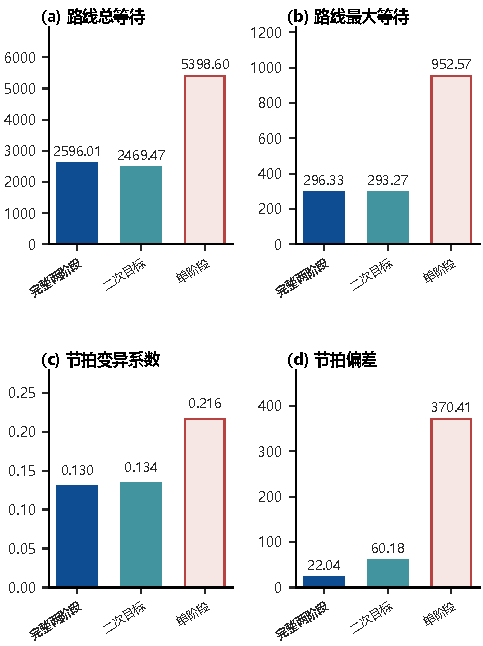
\includegraphics[width=\linewidth]{fig04_workflow_cn_nature}
\caption{历史基准：相同600~s总预算下的排程运行质量。（a）路线总等待时间；（b）路线最大等待时间；（c）节拍变异系数；（d）节拍偏差。三种配置采用相同的20个实例，每种500次运行；纵轴单位依次为s、s、无量纲和s，柱顶为观察均值。}
\label{fig:workflow-zh-new}
\end{figure}
表~\ref{tab:refinement-ablation-zh}分离第二阶段及精修目标形式的影响，与表~\ref{tab:spbs-zh-new}的初始化消融共同评价工作流组件。

\begin{table*}[!htbp]
\centering\scriptsize
\setlength{\tabcolsep}{3pt}
\caption{历史基准：第二阶段及目标形式消融。每个配置包含20个实例、500次运行，总预算均为600~s；表中为实例聚合均值，各指标越小越好。}
\label{tab:refinement-ablation-zh}
\begin{tabular}{ccccc}
\toprule
配置 & 总等待（s） & 最大等待（s） & 节拍CV & 节拍偏差（s）\\
\midrule
完整线性精修 & 2596.01 & 296.33 & 0.130 & 22.04\\
二次目标精修 & 2469.47 & 293.27 & 0.134 & 60.18\\
移除第二阶段 & 5398.60 & 952.57 & 0.216 & 370.41\\
\bottomrule
\end{tabular}
\end{table*}


\subsection{历史基准：SPBS与结构感知割选择}

表~\ref{tab:spbs-zh-new}汇总SPBS配对实验，包含48个实例、每个实例10个配对种子。计时比较评价离线SPBS构造完成后的主求解性能。相对无初始解条件，预计算SPBS将可行解获得率由51.67\%提高至100\%，增加48.33个百分点（95\%区间$[34.58,62.29]$）；平均PDI由27473.05降至20278.78，降低7194.27或26.19\%（95\%区间$[5145.78,9317.61]$）。两项配对差异经Holm校正后仍显著（$p=2.55\times10^{-5}$和$p=3.46\times10^{-8}$）。预计算SPBS提高了后续求解阶段的可行排程获得率，并改善原始--对偶收敛。

\begin{table}[!htbp]
\centering
\scriptsize
\setlength{\tabcolsep}{3pt}
\caption{历史基准：预计算SPBS对限时MILP搜索的影响，计时不含初始解构造。每个条件包含48个实例、每例10个配对种子，共480次运行。}
\label{tab:spbs-zh-new}
\begin{tabular}{cccc}
\toprule
指标 & 无初始解 & SPBS & 观察变化\\
\midrule
可行解获得率（\%） & 51.67 & 100.00 & +48.33个百分点\\
平均PDI & 27473.05 & 20278.78 & -26.19\%\\
\bottomrule
\end{tabular}
\end{table}

HEM-13D是与本文结构感知割选择器最直接的学习型基线。两者共享同一SPBS、训练实例、随机种子、候选上限、隐藏维数和600~s求解预算，每种方法包含500次运行。表~\ref{tab:hem-direct-zh}给出两种策略的配对比较。相对HEM-13D，\method{}的平均PDI由16823.18降至16585.70，平均求解时间由219.65~s降至218.32~s，平均终止相对gap由127.24\%降至126.01\%，证明最优率由62.4\%提高到63.2\%；完整方法的500次运行均获得可行解。按20个制造实例聚合随机重复后，四项配对均值差的95\% bootstrap区间均包含0，Holm校正$p$值均为1.0。相同SPBS条件下，两种学习策略的观察均值接近；配对区间同时覆盖正、负差异，因此本文以观察均值描述该组比较。

\begin{table}[!htbp]
\centering
\scriptsize
\caption{历史基准：共同SPBS和预算下\method{}相对HEM-13D的直接比较。}
\label{tab:hem-direct-zh}
\begin{tabular}{cccc}
\toprule
指标 & HEM-13D & \method{} & 观察变化\\
\midrule
平均PDI & 16823.18 & 16585.70 & -1.41\%\\
平均求解时间（s） & 219.65 & 218.32 & -0.61\%\\
平均终止gap（\%） & 127.24 & 126.01 & -0.97\%\\
证明最优率（\%） & 62.4 & 63.2 & +0.80个百分点\\
\bottomrule
\end{tabular}
\end{table}

该对照在相同初始化和求解预算下联合评价角色感知表示、序列解码与结构补全，量化其在共同SPBS条件下对PDI、求解时间、终止间隙和证明最优率的影响。

\subsection{历史基准：规模、混流构成与求解难度}

析因设计包含$4\times5\times3=60$个产品晶圆数--配方构成--工艺时长系数单元，每个单元使用5个求解器种子，共300次运行。图~\ref{fig:doe-zh-new}显示明显的规模转折：8片和16片各自的75次运行均证明最优，平均PDI分别为28.13和1876.54，平均求解时间为0.34和33.86~s；24片和32片的证明最优率降至36\%和20\%，平均PDI升至31155.94和32959.89，平均求解时间升至408.55和433.20~s。


表~\ref{tab:model-scale-cn}给出析因实验中各规模的模型维度。每个规模包含15个不同参数配置，统计基于预求解前的标量变量和约束，不重复计入求解器种子。16片和24片实例的平均变量数分别为2645.2和6711.2；在采用名义工艺时长的$1{:}1$混流配置下，具体变量数分别为2722和6630。变量数包括布局固定指示量和线性化辅助量，因此描述代数表示规模；独立决策空间还取决于固定关系与工艺约束。

\begin{table*}[t]
\centering
\small
\setlength{\tabcolsep}{5pt}
\caption{历史基准：给定PW布局下析因实验的模型规模。每个规模含15个模型；除变量范围外，各列为均值，一般整数变量数均为0。}
\label{tab:model-scale-cn}
\begin{tabular}{cccccc}
\toprule
产品片数 & 总变量数 & 二元变量数 & 连续变量数 & 总变量范围 & 约束数\\
\midrule
8 & 1163.6 & 644.6 & 519.0 & 892--1450 & 2947.0\\
16 & 2645.2 & 1632.4 & 1012.8 & 2217--3457 & 8727.0\\
24 & 6711.2 & 4962.4 & 1748.8 & 5507--9362 & 23670.8\\
32 & 9984.0 & 7547.2 & 2436.8 & 7801--13663 & 41630.8\\
\bottomrule
\end{tabular}
\end{table*}

代数表示规模与候选次序数量具有不同的增长关系。若资源$r$上有$K_r$个候选动作，成对排序至多引入$\binom{K_r}{2}$个二元量，全部资源对应的数量上界为$\sum_{r\in\mathcal R}\binom{K_r}{2}$；在尚未施加前序关系时，一个资源上的全排列数则为$K_r!$。操作先后关系与资源耦合进一步筛选这些候选次序。因此，二次量级的排序表示仍可编码阶乘量级的候选次序，变量维度与组合搜索规模应分别衡量。

预设PDI析因模型的决定系数$R^2=0.998$，其中上标2为平方记号。在$1{:}1$混合模式条件下，24片和32片的附加交互系数分别为37729.48和40788.63，而工艺时长系数主效应及其预设交互项的95\%区间均包含0。因此，在所测工艺时长系数0.9--1.1范围内，求解难度的观察差异主要与批次规模及混流构成的交互相关，工艺时长系数对应的差异相对较小。

\begin{figure}[!htbp]
\centering
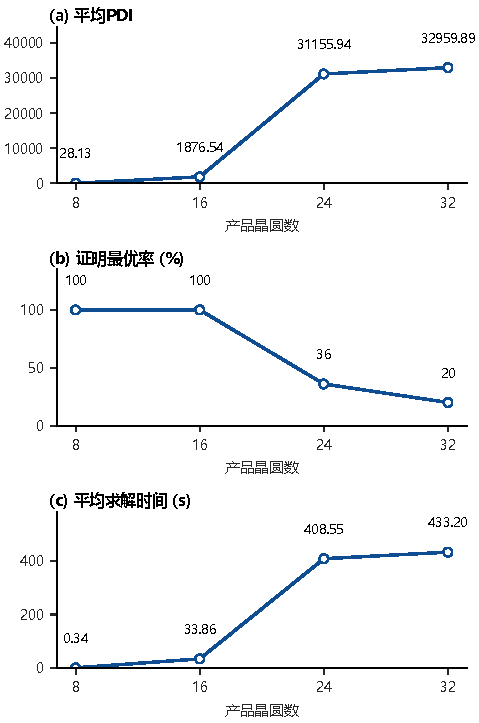
\includegraphics[width=\linewidth]{fig05_doe_cn_nature}
\caption{历史基准：批次规模对求解性能的影响。（a）平均PDI；（b）证明最优率；（c）平均求解时间。横轴为产品晶圆数（片），纵轴单位依次为PDI、\%和s；每个规模包含75次运行，共300次运行。}
\label{fig:doe-zh-new}
\end{figure}

\subsection{历史基准：参数扰动下的可运行性}

既有研究表明，清洁动作及其触发条件会改变CT的机械手动作序列、周期时间和晶圆延迟\citep{yu2020delay,li2022conditioncleaning}。据此，单因素敏感性实验覆盖搬运时长、工艺时长、清洁阈值和真空区辅助晶圆库存的8个预设场景，共80次运行。全部运行均获得并验解可行排程，其中20次证明最优；场景平均PDI位于28899.41--42478.32之间。较长清洁阈值对应最低平均PDI，较慢搬运对应最高平均PDI，反映了所测参数配置下平均搜索表现的差异。

\subsection{历史基准：分布偏移下的可行排程获取}

分布偏移测试把批次扩大到40--64片并改变混流组成，9个制造场景中全部对照方法共形成729次运行，其中完整方法为135次。该实验评价规模与混流组成变化下的排程获取和求解效率。全部729次运行均返回通过原模型约束检验与独立时序核算的可行排程，说明共享SPBS--MILP--SCIP链路在所测规模与配方构成变化下持续输出可验证的排程。该组证明最优率为0\%；完整方法、默认SCIP和自适应评分方法的平均PDI分别为73919.15、73670.99和70915.54。可行排程获取在该组保持100\%，平均PDI则以自适应评分方法最低。

\subsection{历史基准：分型承片约束下的联合排程实验}
\label{sec:joint-evidence-cn}

六个补充配置覆盖6片、$H=3$的单源与双源设备，8片双源的$H=3$与10，以及16片和24片双源的$H=3$。单源辅助晶圆由大气区存储经ATR和装载锁供回，不执行对准；双源辅助晶圆由真空区存储经VTR供回。各配置的两种配方的产品晶圆数量相等，产品依次分布于LP1--LP4，同模式产品允许跨LP配对。辅助晶圆为8片共享库存。VTR输入未完成工艺处理的产品晶圆仅使用两只脏手，输出完成工艺处理的产品晶圆仅使用两只洁净手，辅助晶圆可使用任一空闲手；每个完整承片区间固定占用同一物理手。VTR取片、移动和放片分别为1、2和1~s，旋转为2~s，LL上下槽位属于同一接口，两者之间不另计移动时间。工艺时长为180~s或两次90~s。固定策略按名义工作量向两台腔室分配同模式PW对；联合模型同时选择配对、分腔和周期占位。两者均优化资源次序及事件时刻。

每个配置的五种设置使用完全相同的初始变量赋值，求解器和策略训练种子均为1，初始解构造与辅助变量补全单独计时。固定策略、默认SCIP、HEM和完整选割方法的主求解预算均为300~s；精修设置采用270~s主求解与至多30~s第二阶段；六个精修配置均以默认SCIP为主求解器，与默认SCIP的300~s单阶段结果比较。学习策略沿用固定布局基准的第60轮参数，在联合模型上保持冻结。30个排程均通过完整晶圆路线、工艺处理次数、逐手承载、产品手型、清洁及辅助晶圆复用的独立检查。共同初始解对照中的可行完工时间统一按最后一片产品实际返回原LP的时刻计算。


固定策略在四个6片或8片配置中获得较短的可行完工时间，在16片和24片配置中与联合方法相同。默认SCIP、HEM与完整选割方法的18次联合主求解均保持共同初始解的配对、辅助身份、分腔及加工周期结构，产品完工时间也与初始值相同。该组排程的可行结构由初始化提供，随后时刻精修的收益见表~\ref{tab:joint-refinement-cn}。6片和8片配置各调用学习选割一次，16片与24片配置的调用次数为零；三种联合方法在所测预算内得到相同排程结构和完工时间。固定与联合设置的差异反映其在给定预算下的搜索表现，联合可行域包含对应固定结构子集。

进一步以4片和6片双源混合实例检验固定结构与联合搜索的关系。两种配方的产品数量分别为2:2和3:3，清洁阈值均为$H=10$，共享辅助库存为8片，采用完整候选容量。4片实例在LP1、LP2各放置一片$4\times1$产品，在LP3、LP4各放置一片$2\times2$产品；6片实例在LP1、LP2各放置两种配方的产品各一片，在LP3和LP4分别放置一片$4\times1$和$2\times2$产品。每例的两种设置共用同一完整初始变量赋值，默认SCIP种子为1，主求解上限为1800~s，关闭第二阶段。两例初始化分别耗时0.296和0.781~s，独立于主求解预算。表~\ref{tab:joint-small-cn}同时列出终止下界与可行上界；四个排程均通过完整晶圆路线、逐手承载和辅助复用检查。

\begin{table}[!t]
\centering\scriptsize\setlength{\tabcolsep}{3pt}
\caption{历史基准：小规模双源混合实例的结构对照（$H=10$，时间单位为s）。两种设置的主求解上限均为1800~s；4片固定结构在45~s时上下界收敛。}
% Evidence: results/joint_model/structure_check_20261013_082226; independently checked in results/joint_model_validation/structure_check_20261013/audit.json.
\label{tab:joint-small-cn}
\begin{tabular}{cccccc}\toprule
\multirow{2}{*}{$N$} & \multirow{2}{*}{初始} & \multicolumn{2}{c}{固定结构} & \multicolumn{2}{c}{联合模型}\\
\cmidrule(lr){3-4}\cmidrule(lr){5-6}
 & & 下界 & 上界 & 下界 & 上界\\\midrule
4 & 888 & 532 & 532 & 46 & 717\\
6 & 1530 & 725 & 957 & 39 & 1530\\
\bottomrule\end{tabular}\end{table}

4片固定结构的最优完工时间为532~s，较共同初始排程缩短40.09\%；6片固定结构获得957~s可行排程，较初始排程缩短37.45\%。两次联合求解均保留初始配对、辅助身份、分腔和周期占位；4片实例由888~s改善至717~s，来自既有结构内的时间与资源组织调整。固定结构的532和957~s完整赋值也均满足未固定结构的联合模型约束。因此，这些排程同时给出联合问题的有效可行上界，而表~\ref{tab:joint-small-cn}保留各次独立搜索实际获得的界。两次联合求解分别处理12和3个节点，表明释放结构决策后，该模型在所测预算内的搜索进展较慢。

上述两例的已选结构在两台腔室间重复借用同一组辅助晶圆，每个生产周期均包含D1和D2；同一实体晶圆须先归还再借用，使两腔的相应生产周期依次执行。名义生产负载的均衡并不自动产生腔室并行，辅助身份与借用区间还共同约束可实现的重叠。四个排程均无清洁，其比较对应辅助复用、分型承片与运输时序的耦合。辅助库存总量、实际借用安排和求解所得时序因此需要共同评价。

为进一步检验结构选择的作用，分别以532和957~s固定结构排程启动完整联合模型，保留全部配对、辅助身份、分腔及周期决策自由度，追加1800~s主求解，种子仍为1且关闭第二阶段。两例均保留输入排程的主要结构和完工时间，终止下界分别为46和39~s。表~\ref{tab:joint-auxiliary-cn}给出这两次强初始解验证及辅助身份对照。追加预算与获得初始解的前置求解成本分别计量。

辅助身份对照保持4片实例的产品配对、腔室归属、周期类型、占位和前后侧结构不变，仍使用同一8片共享库存；将CH1的辅助需求分配给D1/D2，将CH2的辅助需求分配给D3/D4。这一对照仅固定新的辅助借用结构，资源次序、物理手分配和事件时刻由MILP优化。以60~s预搜索所得的628~s排程为起点，追加1800~s主求解后得到403~s可行完工时间，终止下界为393~s。该完整变量赋值满足未固定结构的联合模型，因而同时给出4片联合问题的403~s可行上界。

\begin{table}[!t]
\centering\scriptsize\setlength{\tabcolsep}{2.5pt}
\caption{历史基准：强初始解与辅助身份对照（$H=10$，双源，时间单位为s）。追加求解均限时1800~s；原固定结构结果取自表~\ref{tab:joint-small-cn}。末行下界对应固定的新辅助结构。重叠为两腔生产区间交集的总时长；前置构造与求解另行计时。}
% Evidence: results/joint_model/strong_start_20261013_103702; results/joint_model/auxiliary_partition_retry_20261013_103715; results/joint_model_validation/followup_20261013/audit.json.
\label{tab:joint-auxiliary-cn}
\begin{tabular}{cccccc}\toprule
$N$ & 设置 & 起点 & 下界 & 上界 & 重叠\\\midrule
4 & 原固定结构 & 888 & 532 & 532 & 0\\
4 & 联合强初始解 & 532 & 46 & 532 & 0\\
6 & 联合强初始解 & 957 & 39 & 957 & 0\\
4 & 分腔辅助身份 & 628 & 393 & 403 & 111\\
\bottomrule\end{tabular}\end{table}

分腔辅助身份排程中，CH1的$4\times1$工艺处理位于173--353~s，CH2的两次$2\times2$工艺处理位于104--194~s和204--294~s，两腔累计生产重叠111~s。四片产品分别在403、396、347和340~s返回原LP；完整晶圆路线、工艺处理次数、逐手承载和辅助晶圆复用均满足约束，清洁次数为零。403~s低于原辅助借用结构的已证最优值532~s，缩短129~s（24.25\%）。由于原结构内的全部时序安排均受532~s最优值约束，这一严格改善表明，辅助身份调整与随后的时序优化能够突破仅优化原结构时的完工时间。该对照在库存数量不变的条件下量化辅助借用结构的价值；原同初始解算法对照仍按上述共同初始解及300~s总求解预算评价。

精修逐片累计产品晶圆与辅助晶圆的运输路线等待，即相邻搬运或供回片事件间隔扣除必要移动、对准或压力转换时长后的剩余时间。该指标与前述固定布局实验的产品路线等待分别统计。表~\ref{tab:joint-refinement-cn}显示，六个配置的总运输路线等待降低8.40\%--29.21\%，最大单项等待均由73~s降至65~s。6片单源配置的总等待由2200~s降至1680~s，下降23.64\%；实际产品完工时间由3917~s缩短至3875~s。五个双源配置的实际完工时间也均缩短。同为300~s求解总预算，连续时刻精修在所测配置中同时压缩了运输等待和产品完工时间。

\begin{table}[!t]
\centering\scriptsize\setlength{\tabcolsep}{2pt}
\caption{历史基准：分型承片模型的同总预算运输等待精修。时间单位为s；上标(1)/(2)分别表示300~s单阶段与270+至多30~s双阶段。六组均采用默认SCIP；$C_{\max}$按实际产品返回时刻计算。}
\label{tab:joint-refinement-cn}
\begin{tabular}{ccccccc}\toprule
$N$ & 来源 & $H$ & $L_{\rm sum}^{(1)}$ & $L_{\rm sum}^{(2)}$ & 降幅（\%） & $C_{\max}^{(1)}\to C_{\max}^{(2)}$\\\midrule
6 & 双源 & 3 & 356 & 252 & 29.21 & $2051\to1916.91$\\
6 & 单源 & 3 & 2200 & 1680 & 23.64 & $3917\to3875$\\
8 & 双源 & 3 & 532 & 480 & 9.77 & $2300\to2150.96$\\
8 & 双源 & 10 & 524 & 480 & 8.40 & $1779\to1732.96$\\
16 & 双源 & 3 & 1100 & 960 & 12.73 & $4221\to3886.80$\\
24 & 双源 & 3 & 1624 & 1440 & 11.33 & $6823\to6066.30$\\
\bottomrule\end{tabular}\end{table}



双源联合模型的模式扫描覆盖$N=8,16,24$及$H=3,\ldots,10$，每个配置分别采用纯$4\times1$、纯$2\times2$和两种配方产品晶圆数量各半的混合模式。各单元使用至多20~s分层初始搜索和300~s主求解。表~\ref{tab:joint-grid-cn}给出72个通过独立物理检查的可行完工时间，其比较对象是在该预算与初始化策略下获得的排程。

\begin{table}[!t]
\centering\scriptsize\setlength{\tabcolsep}{3pt}
\caption{历史基准：分型承片联合模型在300~s主求解预算下的可行完工时间（s）。混合模式中两种配方的产品晶圆数量相等。}
\label{tab:joint-grid-cn}
\begin{tabular}{ccccc}\toprule
$N$ & $H$ & $4\times1$ & $2\times2$ & 混合\\\midrule
8 & 3 & 1315 & 1658 & 1934\\
8 & 4 & 1315 & 1798 & 1315\\
8 & 5 & 1315 & 1230 & 1264\\
8 & 6 & 1315 & 1318 & 1315\\
8 & 7 & 1315 & 1267 & 1315\\
8 & 8 & 1315 & 1267 & 1227\\
8 & 9 & 1315 & 1267 & 1227\\
8 & 10 & 1315 & 1281 & 1227\\
16 & 3 & 2975 & 4716 & 3423\\
16 & 4 & 2633 & 3470 & 3056\\
16 & 5 & 2633 & 3056 & 2955\\
16 & 6 & 2633 & 2976 & 3055\\
16 & 7 & 2633 & 2874 & 2599\\
16 & 8 & 2633 & 3064 & 2585\\
16 & 9 & 2633 & 2554 & 2585\\
16 & 10 & 2633 & 2591 & 2636\\
24 & 3 & 4640 & 7336 & 5991\\
24 & 4 & 4361 & 6060 & 5359\\
24 & 5 & 4358 & 5434 & 5473\\
24 & 6 & 3945 & 5434 & 4835\\
24 & 7 & 3945 & 4796 & 4835\\
24 & 8 & 3945 & 4799 & 4835\\
24 & 9 & 3945 & 4799 & 4838\\
24 & 10 & 3945 & 4796 & 4203\\
\bottomrule\end{tabular}\end{table}

在所得排程中，8片批次在$H=5,7$时以纯$2\times2$的完工时间最短，在$H=8$--10时以混合模式最短。16片批次的最短观察值在$H=3$--6时来自纯$4\times1$，在$H=7,8$时来自混合模式，在$H=9,10$时来自纯$2\times2$。24片批次则在全部所测$H$下均以纯$4\times1$最短，其完工时间从$H=3$的4640~s降至$H=6$--10的3945~s，降幅为14.98\%。这些差异体现了清洁条件、批量与有限预算搜索共同作用下的排程表现。

为检验两种来源路线，另对2片和4片混合配方产品晶圆、$H=2,3$的八个已有排程进行物理手分配。原排程采用同质手模型、120~s主求解和至多20~s分层初始化；本次保持事件时刻不变，八个排程均能满足洁净手与脏手限制。表~\ref{tab:joint-source-cn}给出复核后的完工时间。2片实例的两个产品采用不同模式，分别与辅助晶圆配对；4片实例实现LP1与LP2、LP3与LP4之间的同模式产品配对。产品经AL和装载锁供回，单源辅助晶圆从大气区存储直接经ATR送入LL，双源辅助晶圆经真空区供回，完整路线、工艺处理次数与共享库存均满足约束。四组配置中，双源排程的可行完工时间均较短。

\begin{table}[!t]\centering\scriptsize\setlength{\tabcolsep}{4pt}
\caption{历史基准：经分型承片复核的单源与双源小规模排程完工时间（s）。单源辅助晶圆不执行对准。}
\label{tab:joint-source-cn}
\begin{tabular}{cccc}\toprule
$N$ & $H$ & 单源 & 双源\\\midrule
2 & 2 & 2378 & 1028\\
2 & 3 & 1433 & 514\\
4 & 2 & 2436 & 1280\\
4 & 3 & 1491 & 854\\
\bottomrule\end{tabular}\end{table}

进一步以8片、$H=3$、双源混合配方产品晶圆检验工艺时长与辅助晶圆库存变化，主求解预算为300~s，初始化预算为20~s。表~\ref{tab:joint-perturb-cn}覆盖名义工艺时长的$\pm10\%$扰动及4、6、10片辅助晶圆库存。五个单元均获得完整可行排程，说明所建模的配对、清洁与运输关系能够在这些输入变化下保持可行。表中数值为各输入下单独搜索所得的完工时间，用于评价排程可获得性。

\begin{table}[!t]\centering\scriptsize\setlength{\tabcolsep}{4pt}
\caption{历史基准：分型承片联合模型的参数扰动结果。时长以s计；两种模式时长分别为单次$4\times1$与单次$2\times2$工艺处理。}
\label{tab:joint-perturb-cn}
\begin{tabular}{cccc}\toprule
$4\times1$时长 & $2\times2$时长 & 辅助库存 & $C_{\max}$\\\midrule
162 & 81 & 8 & 1880\\
198 & 99 & 8 & 1988\\
180 & 90 & 4 & 1875\\
180 & 90 & 6 & 1888\\
180 & 90 & 10 & 1937\\
\bottomrule\end{tabular}\end{table}

表~\ref{tab:order-audit-cn}给出16片、$H=10$时两种纯模式在预求解前的模型维度。物理手分配除引入承片位置选择外，还需表达同一手上承片区间的互斥；对应的手分配变量为672和992个，手占用排序变量为14028和30628个。腔内次序由周期占位、首末参与周期及前后侧状态表示。表中数量包括启用条件、对称选择及可由路线推导的次序，衡量代数表示规模；实际可行组合还受晶圆配对、容量与时序约束共同限制。

在$H=10$、双源、8片辅助且两种配方的产品晶圆数量各半的配置中，16片与24片完整模型分别有124048和296700个变量。仅考虑产品两两配对并分配至两个有标签腔室时，偶数配方数量对应的候选组合数为$N_{\zeta}!N_{\psi}!/[(N_{\zeta}/2)!(N_{\psi}/2)!]$，16片与24片分别为2822400和442597478400。该计数包含标签对称，且尚未施加满片、清洁与晶圆路线限制；它描述指定候选类别的增长，不代表可行排程数或独立变量维度。

\begin{table}[!t]\centering\scriptsize\setlength{\tabcolsep}{4pt}
\caption{历史基准：16片、$H=10$联合模型的规模审计；计数为预处理前候选变量。}
\label{tab:order-audit-cn}
\begin{tabular}{ccc}\toprule
变量类别 & $4\times1$ & $2\times2$\\\midrule
ATR排序 & 4560 & 4560\\
VTR动作排序 & 27730 & 63190\\
VTR手分配 & 672 & 992\\
VTR手占用排序 & 14028 & 30628\\
AL排序 & 120 & 120\\
上LL排序 & 120 & 120\\
下LL排序 & 120 & 120\\
辅助身份借用排序 & 2244 & 5724\\
全部变量 & 78351 & 180925\\
全部约束 & 376764 & 887126\\
\bottomrule\end{tabular}\end{table}



\subsection{历史基准：搜索阶段与强化界诊断}

在8片与16片双源、$H=3$的混合配置上，进一步采用共同可行初始解和相同强化界，分别运行默认SCIP与完整选割方法，各限时120~s。强化界由必要路线与资源占用给出的解析下界以及初始排程的完工时间上界组成。这四次诊断独立于前述300~s算法对照，用于识别搜索预算消耗的阶段。

8片配置中，两种方法均保留2300~s可行排程，终止下界为492~s；均进入根节点的首次LP求解，分别执行25630和24675次LP迭代，尚未触发学习选割。16片配置中，两种方法均保留4221~s可行排程，120~s预算耗用于预处理，处理节点数与LP求解次数均为零。四个最终排程均满足独立物理校验。该诊断将求解时间定位于预处理及根节点松弛阶段，表明本组联合模型的搜索成本首先来自大规模离散表达与连续松弛求解。

\subsection{模式选择与求解性能的讨论}

\paragraph{工艺模式的条件化选择。} 满片要求使假片供回成为生产组织的一部分，模式比较必须同时计入补位、完整链及清洁占位。在历史固定布局的16片批次中，$H=3$时纯$4\times1$以944~s优选，$H=4$时混合配置以939~s优选，$H=6$时纯$2\times2$以898~s优选。这些结果说明选择依据是具体条件下的系统完工时间，而不是仅比较单次工艺时长；其适用范围包括原清洁规则和随阈值重构的预设链布局。现行联合模型应按相同原则比较，但目前上下界未充分分离，不能把历史切换点当作新模型的通用决策规则。

现行规则实验支持三个相互区分的结论：共同初始解帮助本组限时运行获得可行排程；给定主要结构后的时序精修减少等待；辅助身份的结构替换存在严格改善原固定结构最优值的可行排程。结构对照的410~s、精修对照的等待下降和初始化的可行解获取率分别对应不同问题，不能合并为完整联合算法的优越性结论。

扩大清洁选择空间在模型层面包含原规则允许的选择，但限时启发式求解不保证找到更优目标。当前匹配实验未观察到提前清洁改善完工时间，且模式扫描的下界尚不足以确定优选。历史固定布局中由最优值或上下界分离建立的模式排序，仅对其原有规则和设备配置有效。

\paragraph{稳定衔接与工程适用边界。} 同预算精修证明的是在已选结构内压缩等待，不能由此推出驻留方差下降或实现严格JIT。两类硬件偏差说明排程需要跟随参数与状态变化更新，但有限时间内求得确定性可行解也不能证明其在执行偏差下保持可行。若进一步用于现场，应补充动作时长与资源差异的实测描述、偏差发生时的状态继承、重调度延迟及执行约束复验；这些属于后续验证，不纳入本文已完成结果。

新规则下的学习割选择对照未改善共同初始解的主目标；部分运行未触发自定义选择器，触发次数也有限。早期八组精修配置没有有效节拍评价中心；第~\ref{sec:supplement-evidence-cn}节补充的四组有效节拍配置虽降低等待，却未改善节拍偏差，且目标消融未满足起始完整赋值一致的条件。因此仍不能确认节拍项的独立收益。进一步验证需改善对照控制、补足完整模式覆盖及匹配资源预算；未完成的敏感性实验在验收前保持待定。

\FloatBarrier

\section{结论}

本文以满片工艺引入的假片占用为出发点，研究PECVD旋转腔组合设备在不同运行条件下的工艺模式比较与有限预算排程。联合模型将产品配对、假片借用、腔室分配、完整链和清洁边界纳入同一物理时序，用于评价两种预设工艺模式及其混合配置。历史固定布局的16片实验表明，随着清洁阈值变化，优选可以在两种纯模式与混合配置之间切换，因而模式选择必须同时考虑批量、清洁位置和资源衔接；这些切换结论限于相应历史配置。

现行规则下的核心验证、模式扫描及组件消融分别验收112/126、192/216和216/216个有效排程。核心验证的四组匹配配置中，冷启动12次均无可行解超时，串行与SPBS初始解各12次均获得可行排程。八组配置、各三个种子的等预算精修保持产品完工时间，使路线总等待降低22.29\%--50.25\%。4片双源辅助身份对照取得410~s可行排程，低于原固定结构的532~s已证最优值，说明辅助借用关系是影响可达完工时间的实质结构决策。

两阶段模型把减少产品批次完工时间与改善运行衔接分开处理：先在驻留上限等约束下优化产品回片完工时间，再保留其上界并减少等待和周期节拍变化。该优先级为效率与时序质量提供了明确口径，但尚未直接优化驻留一致性。算法以获得并验证有效排程为基础，学习搜索组件的作用需要由相同预算下的结果判定；设备动作时长偏差和资源性能差异则构成继续研究参数更新及在线排程的工程动机。

独立补充批次进一步验收12次固定结构对照、48次有效节拍配置运行、96次清洁规则对照和4次16片可行排程。四组有效节拍配置的等待下降41.53\%--58.50\%，但未观察到超过容差的节拍改善；48组清洁规则配对也未出现完工时间差异。上述证据不支持进一步宣称完整联合问题已求得最优、提前清洁必然缩短完工时间，或学习割选择优于基线。模式扫描存在初始化资源失败，已完成比较的上下界也未分离，敏感性实验尚未形成完整正式比较。历史固定布局与原清洁规则的结果单独保留，不作为这些待验证主张的替代证据。后续工作需改善节拍目标的控制对照、完成保持可行域的规模优化，并补足模式覆盖及新规则下的策略训练与匹配比较。

\section*{CRediT作者贡献声明}
魏林聪负责概念设计、方法设计、软件实现、验证、形式分析、研究实施、数据管理、可视化、初稿撰写以及审阅与编辑；邵立珍负责概念设计、方法设计、形式分析、验证、审阅与编辑以及项目管理；王蔚负责形式分析、研究实施、审阅与编辑以及监督指导。全体作者审阅并批准最终稿。

\section*{利益冲突声明}
作者声明不存在可能影响本文工作的已知财务利益或个人关系。

\section*{数据与研究材料可用性}
支撑本文结果的数据、数学实例、训练模型及求解方法的软件实现可向通讯作者合理申请。

\section*{稿件准备过程中生成式AI和AI辅助技术的声明}
在本稿准备过程中，作者使用OpenAI ChatGPT和Codex辅助语言编辑、中英翻译、LaTeX一致性检查、数值求解方法的实现与调试及实验可视化。使用上述工具后，作者审阅和编辑了相关内容，并对出版物的全部内容承担责任。

\footnotesize
\setlength{\bibsep}{0pt}
\begin{thebibliography}{34}
\expandafter\ifx\csname natexlab\endcsname\relax\def\natexlab#1{#1}\fi
\providecommand{\url}[1]{\texttt{#1}}
\providecommand{\href}[2]{#2}
\providecommand{\path}[1]{#1}
\providecommand{\DOIprefix}{doi:}
\providecommand{\ArXivprefix}{arXiv:}
\providecommand{\URLprefix}{URL: }
\providecommand{\Pubmedprefix}{pmid:}
\providecommand{\doi}[1]{\href{http://dx.doi.org/#1}{\path{#1}}}
\providecommand{\Pubmed}[1]{\href{pmid:#1}{\path{#1}}}
\providecommand{\bibinfo}[2]{#2}
\ifx\xfnm\relax \def\xfnm[#1]{\unskip,\space#1}\fi
%Type = Article
\bibitem[{Pan et~al.(2018)Pan, Zhou, Qiao and Wu}]{pan2018survey}
\bibinfo{author}{Pan, C.R.}, \bibinfo{author}{Zhou, M.C.},
  \bibinfo{author}{Qiao, Y.}, \bibinfo{author}{Wu, N.Q.},
  \bibinfo{year}{2018}.
\newblock \bibinfo{title}{Scheduling cluster tools in semiconductor manufacturing:
  Recent advances and challenges}.
\newblock \bibinfo{journal}{IEEE Transactions on Automation Science and Engineering}
  \bibinfo{volume}{15}, \bibinfo{number}{2}, \bibinfo{pages}{586--601}.
\newblock \DOIprefix\doi{10.1109/TASE.2016.2642997}.
%Type = Article

\bibitem[{{Applied Materials}(n.d.)}]{appliedprecisioncvd}
Applied Materials, n.d.
\newblock Producer XP Precision CVD.
\newblock \url{https://www.appliedmaterials.com/us/en/product-library/producer-xp-precision-cvd.html} (accessed 7 September 2026).

\bibitem[{Gu et~al.(2024)Gu, Wu, Qiao, Zhang and Li}]{gu2024applied}
\bibinfo{author}{Gu, L.}, \bibinfo{author}{Wu, N.},
  \bibinfo{author}{Qiao, Y.}, \bibinfo{author}{Zhang, S.},
  \bibinfo{author}{Li, T.}, \bibinfo{year}{2024}.
\newblock \bibinfo{title}{Scheduling cluster tools with multi-space process
  modules and a multi-finger-arm robot in wafer fabrication subject to wafer
  residency time constraints}.
\newblock \bibinfo{journal}{Applied Sciences} \bibinfo{volume}{14},
  \bibinfo{pages}{9490}.
\newblock \DOIprefix\doi{10.3390/app14209490}.
%Type = Article

\bibitem[{Gu et~al.(2024)Gu, Wu, Qiao and Zhang}]{gu2024multifinger}
\bibinfo{author}{Gu, L.}, \bibinfo{author}{Wu, N.}, \bibinfo{author}{Qiao, Y.},
  \bibinfo{author}{Zhang, S.}, \bibinfo{year}{2024}.
\newblock \bibinfo{title}{Scheduling of {Multi-finger-robotic Cluster Tools}
  with {Multi-space Process Modules}}, in: \bibinfo{booktitle}{2024
  International Conference on Networking, Sensing and Control ({ICNSC})},
  \bibinfo{publisher}{IEEE}.
\newblock \DOIprefix\doi{10.1109/ICNSC62968.2024.10760109}.
%Type = Article

\bibitem[{Perkinson et~al.(1994)Perkinson, McLarty, Gyurcsik and
  Cavin}]{perkinson1994throughput}
\bibinfo{author}{Perkinson, T.L.}, \bibinfo{author}{McLarty, P.K.},
  \bibinfo{author}{Gyurcsik, R.S.}, \bibinfo{author}{Cavin, R.K.},
  \bibinfo{year}{1994}.
\newblock \bibinfo{title}{Single-wafer cluster tool performance: An analysis
  of throughput}.
\newblock \bibinfo{journal}{IEEE Transactions on Semiconductor Manufacturing}
  \bibinfo{volume}{7}, \bibinfo{pages}{369--373}.
\newblock \DOIprefix\doi{10.1109/66.311340}.
%Type = Article

\bibitem[{Rostami and Hamidzadeh(2002)}]{rostami2002optimal}
\bibinfo{author}{Rostami, S.}, \bibinfo{author}{Hamidzadeh, B.},
  \bibinfo{year}{2002}.
\newblock \bibinfo{title}{Optimal scheduling techniques for cluster tools
  with process-module and transport-module residency constraints}.
\newblock \bibinfo{journal}{IEEE Transactions on Semiconductor Manufacturing}
  \bibinfo{volume}{15}, \bibinfo{pages}{341--349}.
\newblock \DOIprefix\doi{10.1109/TSM.2002.801379}.
%Type = Article

\bibitem[{Wu and Zhou(2010)}]{wu2010closedform}
\bibinfo{author}{Wu, N.Q.}, \bibinfo{author}{Zhou, M.C.},
  \bibinfo{year}{2010}.
\newblock \bibinfo{title}{A closed-form solution for schedulability and
  optimal scheduling of dual-arm cluster tools with wafer residency time
  constraint based on steady schedule analysis}.
\newblock \bibinfo{journal}{IEEE Transactions on Automation Science and
  Engineering} \bibinfo{volume}{7}, \bibinfo{pages}{303--315}.
\newblock \DOIprefix\doi{10.1109/TASE.2008.2008633}.
%Type = Article

\bibitem[{Qiao et~al.(2012)Qiao, Wu and Zhou}]{qiao2012sojourn}
\bibinfo{author}{Qiao, Y.}, \bibinfo{author}{Wu, N.Q.},
  \bibinfo{author}{Zhou, M.C.}, \bibinfo{year}{2012}.
\newblock \bibinfo{title}{Petri net modeling and wafer sojourn time analysis
  of single-arm cluster tools with residency time constraints and activity
  time variation}.
\newblock \bibinfo{journal}{IEEE Transactions on Semiconductor Manufacturing}
  \bibinfo{volume}{25}, \bibinfo{pages}{432--446}.
\newblock \DOIprefix\doi{10.1109/TSM.2012.2199338}.
%Type = Article

\bibitem[{Qiao et~al.(2014)Qiao, Wu and Zhou}]{qiao2014revisiting}
\bibinfo{author}{Qiao, Y.}, \bibinfo{author}{Wu, N.},
  \bibinfo{author}{Zhou, M.C.}, \bibinfo{year}{2014}.
\newblock \bibinfo{title}{Scheduling of dual-arm cluster tools with wafer
  revisiting and residency time constraints}.
\newblock \bibinfo{journal}{IEEE Transactions on Industrial Informatics}
  \bibinfo{volume}{10}, \bibinfo{pages}{286--300}.
\newblock \DOIprefix\doi{10.1109/TII.2013.2272702}.
%Type = Article

\bibitem[{Wang et~al.(2020)Wang, Hu, Pan, Zhou and Li}]{wang2020multiple}
\bibinfo{author}{Wang, J.}, \bibinfo{author}{Hu, H.},
  \bibinfo{author}{Pan, C.}, \bibinfo{author}{Zhou, Y.},
  \bibinfo{author}{Li, L.}, \bibinfo{year}{2020}.
\newblock \bibinfo{title}{Scheduling dual-arm cluster tools with multiple
  wafer types and residency time constraints}.
\newblock \bibinfo{journal}{IEEE/CAA Journal of Automatica Sinica}
  \bibinfo{volume}{7}, \bibinfo{pages}{776--789}.
\newblock \DOIprefix\doi{10.1109/JAS.2020.1003150}.
%Type = Article

\bibitem[{Wang et~al.(2025)Wang, Liu, Zhou and
  Abusorrah}]{wang2025virtualcell}
\bibinfo{author}{Wang, J.}, \bibinfo{author}{Liu, C.},
  \bibinfo{author}{Zhou, M.C.}, \bibinfo{author}{Abusorrah, A.},
  \bibinfo{year}{2025}.
\newblock \bibinfo{title}{Virtual cell-based scheduling approach to
  single-robotic-arm cluster tools subject to wafer residency time
  constraints}.
\newblock \bibinfo{journal}{IEEE Transactions on Automation Science and
  Engineering} \bibinfo{volume}{22}, \bibinfo{pages}{240--251}.
\newblock \DOIprefix\doi{10.1109/TASE.2024.3349380}.
%Type = Article

\bibitem[{Yang et~al.(2025)Yang, Li, Zhen, Zhang and Wu}]{yang2025miptwowafers}
\bibinfo{author}{Yang, F.}, \bibinfo{author}{Li, C.}, \bibinfo{author}{Zhen,
  L.}, \bibinfo{author}{Zhang, C.}, \bibinfo{author}{Wu, N.},
  \bibinfo{year}{2025}.
\newblock \bibinfo{title}{Scheduling residency time-constrained single-armed
  cluster tools with two-wafer types via mixed integer programming model}.
\newblock \bibinfo{journal}{Expert Systems with Applications}
  \bibinfo{volume}{288}, \bibinfo{pages}{128209}.
\newblock \DOIprefix\doi{10.1016/j.eswa.2025.128209}.
%Type = Article

\bibitem[{Kim et~al.(2013)Kim, Kim, Lee and Lee}]{kim2013cleaning}
\bibinfo{author}{Kim, H.}, \bibinfo{author}{Kim, H.J.},
  \bibinfo{author}{Lee, J.H.}, \bibinfo{author}{Lee, T.E.},
  \bibinfo{year}{2013}.
\newblock \bibinfo{title}{Scheduling dual-armed cluster tools with cleaning
  processes}.
\newblock \bibinfo{journal}{International Journal of Production Research}
  \bibinfo{volume}{51}, \bibinfo{pages}{3671--3687}.
\newblock \DOIprefix\doi{10.1080/00207543.2012.758392}.
%Type = Article

\bibitem[{Yu and Lee(2020)}]{yu2020delay}
\bibinfo{author}{Yu, T.S.}, \bibinfo{author}{Lee, T.E.},
  \bibinfo{year}{2020}.
\newblock \bibinfo{title}{Wafer delay analysis and control of dual-armed
  cluster tools with chamber cleaning operations}.
\newblock \bibinfo{journal}{International Journal of Production Research}
  \bibinfo{volume}{58}, \bibinfo{pages}{434--447}.
\newblock \DOIprefix\doi{10.1080/00207543.2019.1593547}.
%Type = Article

\bibitem[{Qiao et~al.(2022)Qiao, Lu, Li, Zhang, Wu and Liu}]{qiao2022binary}
\bibinfo{author}{Qiao, Y.}, \bibinfo{author}{Lu, Y.}, \bibinfo{author}{Li, J.},
  \bibinfo{author}{Zhang, S.}, \bibinfo{author}{Wu, N.}, \bibinfo{author}{Liu,
  B.}, \bibinfo{year}{2022}.
\newblock \bibinfo{title}{An efficient binary integer programming model for
  residency time-constrained cluster tools with chamber cleaning requirements}.
\newblock \bibinfo{journal}{IEEE Transactions on Automation Science and
  Engineering} \bibinfo{volume}{19}, \bibinfo{pages}{1757--1771}.
\newblock \DOIprefix\doi{10.1109/TASE.2021.3122576}.
%Type = Article

\bibitem[{Li et~al.(2022)Li, Yang and Zhen}]{li2022conditioncleaning}
\bibinfo{author}{Li, C.}, \bibinfo{author}{Yang, F.}, \bibinfo{author}{Zhen,
  L.}, \bibinfo{year}{2022}.
\newblock \bibinfo{title}{Efficient scheduling approaches to time-constrained
  single-armed cluster tools with condition-based chamber cleaning operations}.
\newblock \bibinfo{journal}{International Journal of Production Research}
  \bibinfo{volume}{60}, \bibinfo{pages}{3555--3568}.
\newblock \DOIprefix\doi{10.1080/00207543.2021.1926568}.
%Type = Inproceedings

\bibitem[{Zhu et~al.(2025)Zhu, Yuan, Wang and Hou}]{zhu2025failuredeadlock}
\bibinfo{author}{Zhu, Q.}, \bibinfo{author}{Yuan, J.},
  \bibinfo{author}{Wang, G.}, \bibinfo{author}{Hou, Y.}, \bibinfo{year}{2025}.
\newblock \bibinfo{title}{Scheduling a single-arm two-cluster tool with a
  process module failure subject to wafer residency time constraints}.
\newblock \bibinfo{journal}{IEEE Transactions on Automation Science and
  Engineering} \bibinfo{volume}{22}, \bibinfo{pages}{667--679}.
\newblock \DOIprefix\doi{10.1109/TASE.2023.3275703}.
%Type = Article

\bibitem[{Kim and Kim(2025)}]{kim2025noncyclicdeadlock}
\bibinfo{author}{Kim, D.}, \bibinfo{author}{Kim, H.J.}, \bibinfo{year}{2025}.
\newblock \bibinfo{title}{Noncyclic scheduling of cluster tools using deep
  reinforcement learning}.
\newblock \bibinfo{journal}{IEEE Transactions on Automation Science and
  Engineering} \bibinfo{volume}{22}, \bibinfo{pages}{24009--24023}.
\newblock \DOIprefix\doi{10.1109/TASE.2025.3632534}.
%Type = Article

\bibitem[{Lee et~al.(2018)Lee, Zhao, Li and Papadopoulos}]{lee2018waiting}
\bibinfo{author}{Lee, J.H.}, \bibinfo{author}{Zhao, C.},
  \bibinfo{author}{Li, J.}, \bibinfo{author}{Papadopoulos, C.T.},
  \bibinfo{year}{2018}.
\newblock \bibinfo{title}{Analysis, design, and control of {Bernoulli}
  production lines with waiting time constraints}.
\newblock \bibinfo{journal}{Journal of Manufacturing Systems}
  \bibinfo{volume}{46}, \bibinfo{pages}{208--220}.
\newblock \DOIprefix\doi{10.1016/j.jmsy.2018.01.001}.
%Type = Article

\bibitem[{Weng et~al.(2022)Weng, Chen, Zheng and Fujimura}]{weng2022jit}
Weng, W., Chen, J., Zheng, M., Fujimura, S., 2022.
\newblock Realtime scheduling heuristics for just-in-time production in large-scale flexible job shops.
\newblock Journal of Manufacturing Systems 63, 64--77.
\newblock \DOIprefix\doi{10.1016/j.jmsy.2022.01.006}.

\bibitem[{Rahmani and Heydari(2014)}]{rahmani2014robust}
Rahmani, D., Heydari, M., 2014.
\newblock Robust and stable flow shop scheduling with unexpected arrivals of new jobs and uncertain processing times.
\newblock Journal of Manufacturing Systems 33, 84--92.
\newblock \DOIprefix\doi{10.1016/j.jmsy.2013.03.004}.

\bibitem[{Kim and Lee(2025)}]{kim2025adaptivecluster}
\bibinfo{author}{Kim, H.J.}, \bibinfo{author}{Lee, J.H.}, \bibinfo{year}{2025}.
\newblock \bibinfo{title}{Scheduling cluster tools for concurrent processing:
  Deep reinforcement learning with adaptive search}.
\newblock \bibinfo{journal}{IEEE Transactions on Automation Science and
  Engineering} \bibinfo{volume}{22}, \bibinfo{pages}{3783--3796}.
\newblock \DOIprefix\doi{10.1109/TASE.2024.3399818}.
%Type = Article

\bibitem[{Tang et~al.(2020)Tang, Agrawal and Faenza}]{tang2020cut}
\bibinfo{author}{Tang, Y.}, \bibinfo{author}{Agrawal, S.},
  \bibinfo{author}{Faenza, Y.}, \bibinfo{year}{2020}.
\newblock \bibinfo{title}{Reinforcement learning for integer programming:
  Learning to cut}, in: \bibinfo{booktitle}{Proceedings of the 37th
  International Conference on Machine Learning}, \bibinfo{publisher}{PMLR}. pp.
  \bibinfo{pages}{9367--9376}.
\newblock \URLprefix \url{https://proceedings.mlr.press/v119/tang20a.html}.
%Type = Article

\bibitem[{Huang et~al.(2022)Huang, Wang, Liu, Zhen, Zhang, Yuan, Hao, Yu and
  Wang}]{huang2022cutranking}
\bibinfo{author}{Huang, Z.}, \bibinfo{author}{Wang, K.}, \bibinfo{author}{Liu,
  F.}, \bibinfo{author}{Zhen, H.L.}, \bibinfo{author}{Zhang, W.},
  \bibinfo{author}{Yuan, M.}, \bibinfo{author}{Hao, J.}, \bibinfo{author}{Yu,
  Y.}, \bibinfo{author}{Wang, J.}, \bibinfo{year}{2022}.
\newblock \bibinfo{title}{Learning to select cuts for efficient mixed-integer
  programming}.
\newblock \bibinfo{journal}{Pattern Recognition} \bibinfo{volume}{123},
  \bibinfo{pages}{108353}.
\newblock \DOIprefix\doi{10.1016/j.patcog.2021.108353}.
%Type = Inproceedings

\bibitem[{Paulus et~al.(2022)Paulus, Zarpellon, Krause, Charlin and
  Maddison}]{paulus2022looking}
\bibinfo{author}{Paulus, M.B.}, \bibinfo{author}{Zarpellon, G.},
  \bibinfo{author}{Krause, A.}, \bibinfo{author}{Charlin, L.},
  \bibinfo{author}{Maddison, C.}, \bibinfo{year}{2022}.
\newblock \bibinfo{title}{Learning to cut by looking ahead: Cutting plane
  selection via imitation learning}, in: \bibinfo{booktitle}{Proceedings of the
  39th International Conference on Machine Learning},
  \bibinfo{publisher}{PMLR}. pp. \bibinfo{pages}{17584--17600}.
\newblock \URLprefix \url{https://proceedings.mlr.press/v162/paulus22a.html}.
%Type = Inproceedings

\bibitem[{Wang et~al.(2023)Wang, Li, Wang, Kuang, Yuan, Zeng, Zhang and
  Wu}]{wang2023hem}
\bibinfo{author}{Wang, Z.}, \bibinfo{author}{Li, X.}, \bibinfo{author}{Wang,
  J.}, \bibinfo{author}{Kuang, Y.}, \bibinfo{author}{Yuan, M.},
  \bibinfo{author}{Zeng, J.}, \bibinfo{author}{Zhang, Y.}, \bibinfo{author}{Wu,
  F.}, \bibinfo{year}{2023}.
\newblock \bibinfo{title}{Learning cut selection for mixed-integer linear
  programming via hierarchical sequence model}, in:
  \bibinfo{booktitle}{Proceedings of the Eleventh International Conference on
  Learning Representations}.
\newblock \URLprefix \url{https://openreview.net/forum?id=Zob4P9bRNcK}.
%Type = Article

\bibitem[{Achterberg(2009)}]{achterberg2009scip}
\bibinfo{author}{Achterberg, T.}, \bibinfo{year}{2009}.
\newblock \bibinfo{title}{{SCIP}: Solving constraint integer programs}.
\newblock \bibinfo{journal}{Mathematical Programming Computation}
  \bibinfo{volume}{1}, \bibinfo{pages}{1--41}.
\newblock \DOIprefix\doi{10.1007/s12532-008-0001-1}.
%Type = Article

\bibitem[{Bestuzheva et~al.(2023)Bestuzheva, Besan{\c{c}}on, Chen, Chmiela,
  Donkiewicz, van Doornmalen, Eifler, Gaul, Gamrath, Gleixner, Gottwald,
  Graczyk, Halbig, Hoen, Hojny, van~der Hulst, Koch, L{\"u}bbecke, Maher,
  Matter, M{\"u}hmer, M{\"u}ller, Pfetsch, Schl{\"o}sser, Serrano, Shinano,
  Sofranac, Turner, Vigerske, Wegscheider, Wellner, Weninger and
  Witzig}]{bestuzheva2023scip}
\bibinfo{author}{Bestuzheva, K.}, \bibinfo{author}{Besan{\c{c}}on, M.},
  \bibinfo{author}{Chen, W.K.}, \bibinfo{author}{Chmiela, A.},
  \bibinfo{author}{Donkiewicz, T.}, \bibinfo{author}{van Doornmalen, J.},
  \bibinfo{author}{Eifler, L.}, \bibinfo{author}{Gaul, O.},
  \bibinfo{author}{Gamrath, G.}, \bibinfo{author}{Gleixner, A.},
  \bibinfo{author}{Gottwald, L.}, \bibinfo{author}{Graczyk, C.},
  \bibinfo{author}{Halbig, K.}, \bibinfo{author}{Hoen, A.},
  \bibinfo{author}{Hojny, C.}, \bibinfo{author}{van~der Hulst, R.},
  \bibinfo{author}{Koch, T.}, \bibinfo{author}{L{\"u}bbecke, M.E.},
  \bibinfo{author}{Maher, S.J.}, \bibinfo{author}{Matter, F.},
  \bibinfo{author}{M{\"u}hmer, E.}, \bibinfo{author}{M{\"u}ller, B.},
  \bibinfo{author}{Pfetsch, M.E.}, \bibinfo{author}{Schl{\"o}sser, F.},
  \bibinfo{author}{Serrano, F.}, \bibinfo{author}{Shinano, Y.},
  \bibinfo{author}{Sofranac, B.}, \bibinfo{author}{Turner, M.},
  \bibinfo{author}{Vigerske, S.}, \bibinfo{author}{Wegscheider, F.},
  \bibinfo{author}{Wellner, P.}, \bibinfo{author}{Weninger, D.},
  \bibinfo{author}{Witzig, J.}, \bibinfo{year}{2023}.
\newblock \bibinfo{title}{Enabling research through the {SCIP} optimization
  suite 8.0}.
\newblock \bibinfo{journal}{ACM Transactions on Mathematical Software}
  \bibinfo{volume}{49}, \bibinfo{pages}{22:1--22:21}.
\newblock \DOIprefix\doi{10.1145/3585516}.
%Type = Inproceedings

\bibitem[{Wang et~al.(2024)Wang, Wang, Li, Kuang, Shi, Zhu, Yuan, Zeng, Zhang and Wu}]{wang2024hemset}
Wang, J., Wang, Z., Li, X., Kuang, Y., Shi, Z., Zhu, F., Yuan, M., Zeng, J., Zhang, Y., Wu, F., 2024.
\newblock Learning to Cut via Hierarchical Sequence/Set Model for Efficient Mixed-Integer Programming.
\newblock arXiv:2404.12638.
\newblock \URLprefix \url{https://arxiv.org/abs/2404.12638}.

\bibitem[{Vinyals et~al.(2015)Vinyals, Fortunato and
  Jaitly}]{vinyals2015pointer}
\bibinfo{author}{Vinyals, O.}, \bibinfo{author}{Fortunato, M.},
  \bibinfo{author}{Jaitly, N.}, \bibinfo{year}{2015}.
\newblock \bibinfo{title}{Pointer networks}, in: \bibinfo{booktitle}{Advances
  in Neural Information Processing Systems}, pp. \bibinfo{pages}{2692--2700}.
%Type = Inproceedings

\bibitem[{Choo et~al.(2022)Choo, Kwon, Kim, Jae, Hottung, Tierney and
  Gwon}]{choo2022beam}
\bibinfo{author}{Choo, J.}, \bibinfo{author}{Kwon, Y.D.}, \bibinfo{author}{Kim,
  J.}, \bibinfo{author}{Jae, J.}, \bibinfo{author}{Hottung, A.},
  \bibinfo{author}{Tierney, K.}, \bibinfo{author}{Gwon, Y.},
  \bibinfo{year}{2022}.
\newblock \bibinfo{title}{Simulation-guided beam search for neural
  combinatorial optimization}, in: \bibinfo{booktitle}{Advances in Neural
  Information Processing Systems}.
\newblock \URLprefix
  \url{https://papers.nips.cc/paper_files/paper/2022/hash/39b9b60f0d149eabd1fff2d7c7d5afc4-Abstract-Conference.html},
  \DOIprefix\doi{10.52202/068431-0637}.
%Type = Article

\bibitem[{Nemhauser et~al.(1978)Nemhauser, Wolsey and
  Fisher}]{nemhauser1978analysis}
\bibinfo{author}{Nemhauser, G.L.}, \bibinfo{author}{Wolsey, L.A.},
  \bibinfo{author}{Fisher, M.L.}, \bibinfo{year}{1978}.
\newblock \bibinfo{title}{An analysis of approximations for maximizing
  submodular set functions---i}.
\newblock \bibinfo{journal}{Mathematical Programming} \bibinfo{volume}{14},
  \bibinfo{pages}{265--294}.
\newblock \DOIprefix\doi{10.1007/BF01588971}.
%Type = Article

\bibitem[{Williams(1992)}]{williams1992reinforce}
\bibinfo{author}{Williams, R.J.}, \bibinfo{year}{1992}.
\newblock \bibinfo{title}{Simple statistical gradient-following algorithms for
  connectionist reinforcement learning}.
\newblock \bibinfo{journal}{Machine Learning} \bibinfo{volume}{8},
  \bibinfo{pages}{229--256}.
\newblock \DOIprefix\doi{10.1007/BF00992696}.
%Type = Inproceedings

\bibitem[{Mnih et~al.(2016)Mnih, Badia, Mirza, Graves, Lillicrap, Harley,
  Silver and Kavukcuoglu}]{mnih2016a3c}
\bibinfo{author}{Mnih, V.}, \bibinfo{author}{Badia, A.P.},
  \bibinfo{author}{Mirza, M.}, \bibinfo{author}{Graves, A.},
  \bibinfo{author}{Lillicrap, T.P.}, \bibinfo{author}{Harley, T.},
  \bibinfo{author}{Silver, D.}, \bibinfo{author}{Kavukcuoglu, K.},
  \bibinfo{year}{2016}.
\newblock \bibinfo{title}{Asynchronous methods for deep reinforcement
  learning}, in: \bibinfo{booktitle}{Proceedings of the 33rd International
  Conference on Machine Learning}, \bibinfo{publisher}{PMLR}. pp.
  \bibinfo{pages}{1928--1937}.
\newblock \URLprefix \url{https://proceedings.mlr.press/v48/mniha16.html}.

\end{thebibliography}

\end{document}

